\documentclass[letterpaper,10pt]{book}
% Change to 10 pt
\usepackage{pdfpages}
\usepackage{morewrites}			% to counteract the no write space problem
\setcounter{tocdepth}{6}

\usepackage[framemethod=TikZ]{mdframed}

\usepackage{fancyhdr}

\usepackage{paralist}
\usepackage{amsmath}
\usepackage{amsfonts}
\usepackage{amssymb}
\usepackage{graphicx}

\usepackage{datetime}
%\usepackage{ulem}

%\usepackage[nottoc]{toobibind}

\usepackage[inline]{enumitem}

% Outer margin at 2.50 is exacty correct to fit the ``corruption alert'' tables
\usepackage[inner=1.0in, outer=2.50in, top=2.54cm,bottom=2.54cm, marginparwidth=2.25in]{geometry}

\usepackage{marginnote}
\usepackage{longtable}
\usepackage{booktabs}
\usepackage{xcolor}

\usepackage{soul}

%%%%%%%%%%%%
\definecolor{ForestGreen}{rgb}{0.00,0.29,0.098}
%%%%%%%%%%%%

\usepackage{marginnote}

\usepackage{imakeidx} 
\usepackage[
	backref=true,
	style=numeric,
%	citestyle=numeric,
	backend=bibtex
	]{biblatex}
\usepackage[driverfallback=hypertex,colorlinks=True]{hyperref}
\usepackage{cleveref}

\makeindex[name=scripture,columnsep=20pt, columnseprule=True,columns=3, title=Scripture References]
\makeindex[name=speaker,columnsep=20pt, columnseprule=True,,columns=2, title=Sermon Creator]
\makeindex[name=series,columnsep=20pt, columnseprule=True,,columns=2, title=Sermon Series]
\makeindex[name=date,columnsep=20pt, columnseprule=True,columns=2, title=Sermon Date]
\makeindex[name=event,columnsep=20pt, columnseprule=True,columns=2, title=Event]
\makeindex[name=topic,columnsep=20pt, columnseprule=True,columns=2, title=Topic]
\makeindex[name=AWIP,columnsep=20pt, columnseprule=True,columns=3, title=All Words in Passage]
\makeindex[name=NWIV,columnsep=20pt, columnseprule=True,columns=3, title=Number of Words in Verse]
\makeindex[name=PNIP,columnsep=20pt, columnseprule=True,columns=3, title=Proper Names in Passage]
\makeindex[name=PEIP,columnsep=20pt, columnseprule=True,columns=2, title=Prophetic Events in Passage]
\makeindex[name=TWPAQ,columnsep=20pt, columnseprule=True,columns=1, title=13-Word Phrases and Quotes]
\makeindex[name=PFTTIS,columnsep=20pt, columnseprule=False,columns=3, title=Phrases found 13 times in scripture]
\makeindex[name=WFTTIS,columnsep=20pt, columnseprule=False,columns=3, title=Words found 13 times in scripture]
\makeindex[name=WFITV,columnsep=20pt, columnseprule=False,columns=3, title=Words found in exactly 13 verses]
\makeindex[name=EVENTS,columnsep=20pt, columnseprule=False,columns=2, title=Sermon Log by Place]
\makeindex[name=QUESTIONS,columnsep=20pt, columnseprule=False,columns=2, title=Bible Questions]
\makeindex[name=DOCTRINES,columnsep=20pt, columnseprule=False,columns=2, title=Doctrines]
\makeindex[name=SONGS,columnsep=20pt, columnseprule=False,columns=1, title=Songs]
\makeindex[name=LOCATION,columnsep=20pt, columnseprule=False,columns= 2, title=Location]
\makeindex[name=FACEBOOK,columnsep=20pt, columnseprule=False,columns=2, title=Facebook]
\makeindex[name=DEVOTIONAL,columnsep=20pt, columnseprule=False,columns=2, title=Devotional Items]
%%%%%%%%%%%%%%%%% EXTRA COLORS
\definecolor{champagne}{rgb}{0.97,0.91,0.81}
\definecolor{bone}{rgb}{0.89,0.85,0.79}
\pagestyle{fancy}
\fancyhf{}
\fancyhead[LE,RO]{\today}
\fancyhead[RE,LO]{Daily Bible Reading}
\fancyhead[CE,CO]{-page \thepage  - }

\fancyfoot[CO,CE]{\leftmark}
%\fancyfoot[LE,RO]{CSCE 692, HW1}

\title{DBR\\
Daily \\ Reads}
\author{Keith Anthony \\
\today }
%+/ffffff +   \pagenumbering{gobble}
\bibliography{Bibliographies/All20220122}

\setlength{\fboxsep}{1.0pt}

\usepackage[utf8]{inputenc}
\usepackage{tikz}

\begin{document}
%%%%%%%%%%%% Tile Page

\begin{titlepage}

\begin{flushright}
\rightskip=-2.5cm
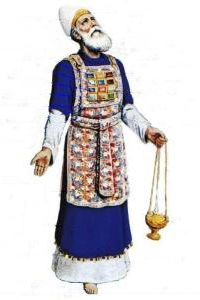
\includegraphics[width=50mm,scale=1.5]{Extras/Melchisedec.jpg}
\vspace{0.4in}  % Create a title for the document and write it in bold font
\LARGE{\textbf{\date}} % Again, do a line break
\linebreak 
% Create a subtitle \large{with Outlines, Statistics, Cross References, and Notes}
\vspace{0.5in}
\begin{flushleft}
\LARGE{Day \#69: Thursday, 10 March 2022 LITE \\}\vspace{0.25in}
\LARGE{Joshua 13-15 Psalm 69 Proverb 10}
\end{flushleft}
\vspace{0.6in}
\bigskip

\normalsize{Xenia, Oh.\\}
\normalsize{created: \today}
\vspace{1.3in}

\end{flushright}
\end{titlepage}

\newpage 
\tableofcontents\hypertarget{TOC}{}
\listoffigures
\listoftables

\hyphenation{A-bim-e-lech bre-thren E-phra-im  Gib-e-o-nites Jer-u-sa-lem through-out Phil-i-stines The-o-phil-us Am-a-le-kites ven-geance Mesh-el-e-mi-ah onan-ism Phar-a-oh thoughts grev-ous-ness Hach-a-liah adul-ter-er Shad-rach}

%%%%%%%%%%%%%%%%% EXTRA COLORS
%%%%%%%%%%%%%%%%% EXTRA COLORS
%%%%%%%%%%%%%%%%% EXTRA COLORS
\definecolor{champagne}{rgb}{0.97,0.91,0.81}
\definecolor{bone}{rgb}{0.89,0.85,0.79}

\definecolor{ForestGreen}{rgb}{0.00,0.29,0.098}
\definecolor{GIVING}{cmyk}{1,0.0,0.72,.1}

\definecolor{MLPE}{cmyk}{1,1,0,.45}
\definecolor{SOCCER}{cmyk}{.77, 0, .42, .49}
\definecolor{PAYBILL}{cmyk}{0,0.83,0.76,0.07}
\definecolor{SERMON}{cmyk}{.14,.9,0,.30} % aka seance \href{http://www.flatuicolorpicker.com/purple-cmyk-color-model/}{seance}
\definecolor{BIBLE}{cmyk}{0,.17,.74,.17}
\definecolor{WORKBLUE}{cmyk}{1, .5, 0, .6}
\definecolor{myOrange}{cmyk}{0, .4, .98, .03}
\definecolor{myTan}{cmyk}{0.0,.07,.17,.10}
\definecolor{myRed}{cmyk}{0,1,1,0}
\definecolor{myWhite}{cmyk}{0,0,0,0}
\definecolor{BLUESoD}{cmyk}{.97,.84,0,.04}
\definecolor{WHITE}{cmyk}{0,0,0,0}
\definecolor{OLDGOLD}{cmyk}{0.05,0.3,1.00,0}
\definecolor{CASTLETON}{cmyk}{1,0,0.31,0.66}
\definecolor{cadmiumgreen}{rgb}{0.0, 0.42, 0.24}
\definecolor{jungle}{rgb}{0.203,0.4882,0.1718}
\definecolor{MYGOLD}{rgb}{1,.84,0}

\definecolor{MYLIGHTGRAY}{rgb}{.85,.85,.85}

\definecolor{codegreen}{rgb}{0,0.6,0}
\definecolor{codegray}{rgb}{0.5,0.5,0.5}
\definecolor{codepurple}{rgb}{0.58,0,0.82}
\definecolor{backcolour}{rgb}{0.95,0.95,0.92}


\mdfdefinestyle{MyFrame}{%
    linecolor=blue,
    outerlinewidth=2pt,
    roundcorner=5pt,
    innertopmargin=\baselineskip,
    innerbottommargin=\baselineskip,
    innerrightmargin=10pt,
    innerleftmargin=10pt,
    backgroundcolor=gray!25!white}


\mdfdefinestyle{MyFrame2}{%
    linecolor=black,
    outerlinewidth=2pt,
    roundcorner=5pt,
    innertopmargin=\baselineskip,
    innerbottommargin=\baselineskip,
    innerrightmargin=10pt,
    innerleftmargin=10pt,
    backgroundcolor=yellow!25!white}


%%%%%
%% for PFTTIS list
%%%%%

%%% And Joseph said unto
\index[PFTTIS]{And Joseph said unto!Genesis!Gen 40:008}
\index[PFTTIS]{And Joseph said unto!Genesis!Gen 40:012}
\index[PFTTIS]{And Joseph said unto!Genesis!Gen 41:025}
\index[PFTTIS]{And Joseph said unto!Genesis!Gen 42:014}
\index[PFTTIS]{And Joseph said unto!Genesis!Gen 42:018}
\index[PFTTIS]{And Joseph said unto!Genesis!Gen 44:015}
\index[PFTTIS]{And Joseph said unto!Genesis!Gen 45:003}
\index[PFTTIS]{And Joseph said unto!Genesis!Gen 45:004}
\index[PFTTIS]{And Joseph said unto!Genesis!Gen 46:031}
\index[PFTTIS]{And Joseph said unto!Genesis!Gen 48:009}
\index[PFTTIS]{And Joseph said unto!Genesis!Gen 48:018}
\index[PFTTIS]{And Joseph said unto!Genesis!Gen 50:019}
\index[PFTTIS]{And Joseph said unto!Genesis!Gen 50:024}


%%% a shadow
\index[PFTTIS]{a shadow!1Chronicles!1Chr 029:15}
\index[PFTTIS]{a shadow!Job!Job 008:09}
\index[PFTTIS]{a shadow!Job!Job 014:02}
\index[PFTTIS]{a shadow!Job!Job 017:07}
\index[PFTTIS]{a shadow!Psalm!Psa 102:011}
\index[PFTTIS]{a shadow!Psalm!Psa 144:004}
\index[PFTTIS]{a shadow!Ecclesiastes!Eccl 006:012}
\index[PFTTIS]{a shadow!Ecclesiastes!Eccl 008:013}
\index[PFTTIS]{a shadow!Isaiah!Isa 04:006}
\index[PFTTIS]{a shadow!Isaiah!Isa 25:004}
\index[PFTTIS]{a shadow!Jonah!Jnh 04:06}
\index[PFTTIS]{a shadow!Colossians!Col 02:017}
\index[PFTTIS]{a shadow!Hebews!Heb 10:001}

%%% blessed is the man
\index[PFTTIS]{blessed is the man!Psalm!Psa 001:001}
\index[PFTTIS]{blessed is the man!Psalm!Psa 032:002}
\index[PFTTIS]{blessed is the man!Psalm!Psa 034:008}
\index[PFTTIS]{blessed is the man!Psalm!Psa 065:004}
\index[PFTTIS]{blessed is the man!Psalm!Psa 084:005}
\index[PFTTIS]{blessed is the man!Psalm!Psa 084:012}
\index[PFTTIS]{blessed is the man!Psalm!Psa 094:012}
\index[PFTTIS]{blessed is the man!Psalm!Psa 112:001}
\index[PFTTIS]{blessed is the man!Proverbs!Pro 008:034}
\index[PFTTIS]{blessed is the man!Isaiah!Isa 056:002}
\index[PFTTIS]{blessed is the man!Jeremiah!Jer 017:007}
\index[PFTTIS]{blessed is the man!Romans!Rom 004:008}
\index[PFTTIS]{blessed is the man!James!Jam 001:012}


%%% carry them
\index[PFTTIS]{carry them!Leviticus!Lev 14:045}
\index[PFTTIS]{carry them!Numbers!Num 11:012}
\index[PFTTIS]{carry them!Joshua!Jsh 04:003}
\index[PFTTIS]{carry them!1Samuel!1Sam 20:040}
\index[PFTTIS]{carry them!1Kings!1Kng 08:046}
\index[PFTTIS]{carry them!2Chronicles!2Chr 06:036}
\index[PFTTIS]{carry them!Ezra!Ezra 05:015}
\index[PFTTIS]{carry them!Isaiah!Isa 40:011}
\index[PFTTIS]{carry them!Isaiah!Isa 41:016}
\index[PFTTIS]{carry them!Isaiah!Isa 57:013}
\index[PFTTIS]{carry them!Jeremiah!Jer 20:004}
\index[PFTTIS]{carry them!Jeremiah!Jer 20:005}
\index[PFTTIS]{carry them!Jeremiah!Jer 43:012}


\index[PFTTIS]{good tidings!2Samuel!2Sam 18:027}
\index[PFTTIS]{good tidings!1Kings!1Ki 01:042}
\index[PFTTIS]{good tidings!2Kings!2Ki 07:009 (2x)}
\index[PFTTIS]{good tidings!Isaiah!Isa 40:009 (2x)}
\index[PFTTIS]{good tidings!Isaiah!Isa 41:007}
\index[PFTTIS]{good tidings!Isaiah!Isa 52:007}
\index[PFTTIS]{good tidings!Isaiah!Isa 61:001}
\index[PFTTIS]{good tidings!Nahum!Nah 01:005}
\index[PFTTIS]{good tidings!Luke!Lk 02:010}
\index[PFTTIS]{good tidings!1Thessalonians!1Thess 03:006}


%%% dead body
\index[PFTTIS]{dead body!Leviticus!Lev 21:011}
\index[PFTTIS]{dead body!Numbers!Num 06:006}
\index[PFTTIS]{dead body!Numbers!Num 09:006}
\index[PFTTIS]{dead body!Numbers!Num 09:007}
\index[PFTTIS]{dead body!Numbers!Num 09:010}
\index[PFTTIS]{dead body!Numbers!Num 09:011}
\index[PFTTIS]{dead body!Numbers!Num 09:013}
\index[PFTTIS]{dead body!Numbers!Num 09:016}
\index[PFTTIS]{dead body!2Kings!2Ki 08:005}
\index[PFTTIS]{dead body!Isaiah!Isa 26:019}
\index[PFTTIS]{dead body!Jeremiah!Jer 26:023}
\index[PFTTIS]{dead body!Jeremiah!Jer 36:030}
\index[PFTTIS]{dead body!Haggai!Hag 02:013}

%%% great sea
\index[PFTTIS]{great sea!Numbers!Num 34:006}
\index[PFTTIS]{great sea!Numbers!Num 34:007}
\index[PFTTIS]{great sea!Joshua!Jos 01:004}
\index[PFTTIS]{great sea!Joshua!Jos 09:001}
\index[PFTTIS]{great sea!Joshua!Jos 15:012}
\index[PFTTIS]{great sea!Joshua!Jos 15:047}
\index[PFTTIS]{great sea!Joshua!Jos 23:004}
\index[PFTTIS]{great sea!Ezekiel!Eze 47:010}
\index[PFTTIS]{great sea!Ezekiel!Eze 47:015}
\index[PFTTIS]{great sea!Ezekiel!Eze 47:019}
\index[PFTTIS]{great sea!Ezekiel!Eze 47:020}
\index[PFTTIS]{great sea!Ezekiel!Eze 48:028}
\index[PFTTIS]{great sea!Daniel!Dan 07:002}


%%% have forsaken me
\index[PFTTIS]{have forsaken me!Judges!Jdg 10:013}
\index[PFTTIS]{have forsaken me!1Samuel!1Sam 08:008}
\index[PFTTIS]{have forsaken me!1Kings!1Ki 11:033}
\index[PFTTIS]{have forsaken me!2Kings!2Ki 22:017}
\index[PFTTIS]{have forsaken me!2Chronicles!2Chr 12:005}
\index[PFTTIS]{have forsaken me!2Chronicles!2Chr 34:025}
\index[PFTTIS]{have forsaken me!Jeremiah!Jer 01:016}
\index[PFTTIS]{have forsaken me!Jeremiah!Jer 02:013}
\index[PFTTIS]{have forsaken me!Jeremiah!Jer 05:007}
\index[PFTTIS]{have forsaken me!Jeremiah!Jer 05:019}
\index[PFTTIS]{have forsaken me!Jeremiah!Jer 16:011 (2x)}
\index[PFTTIS]{have forsaken me!Jeremiah!Jer 19:004}

%%% no king
\index[PFTTIS]{no king!Judges!Jdg 17:06}
\index[PFTTIS]{no king!Judges!Jdg 18:01}
\index[PFTTIS]{no king!Judges!Jdg 19:01}
\index[PFTTIS]{no king!Judges!Jdg 21:25}
\index[PFTTIS]{no king!1Kings!1Ki 22:47}
\index[PFTTIS]{no king!2Kings!2Ki 23:25}
\index[PFTTIS]{no king!Nehemiah!Neh 13:26}
\index[PFTTIS]{no king!Psalms!Psa 033:016}
\index[PFTTIS]{no king!Proverbs!Pro 30:27}
\index[PFTTIS]{no king!Daniel!Dan 02:10}
\index[PFTTIS]{no king!Hosea!Hos 10:03}
\index[PFTTIS]{no king!Micah!Mic 04:09}
\index[PFTTIS]{no king!John!Jhn 19:15}


%%% rebellious house
\index[PFTTIS]{rebellious house!Exodus!Exo 02:005}
\index[PFTTIS]{rebellious house!Exodus!Exo 02:006}
\index[PFTTIS]{rebellious house!Exodus!Exo 02:008}
\index[PFTTIS]{rebellious house!Exodus!Exo 03:009}
\index[PFTTIS]{rebellious house!Exodus!Exo 03:026}
\index[PFTTIS]{rebellious house!Exodus!Exo 03:027}
\index[PFTTIS]{rebellious house!Exodus!Exo 12:002 (2x)}
\index[PFTTIS]{rebellious house!Exodus!Exo 12:003}
\index[PFTTIS]{rebellious house!Exodus!Exo 12:009}
\index[PFTTIS]{rebellious house!Exodus!Exo 12:025}
\index[PFTTIS]{rebellious house!Exodus!Exo 17:012}
\index[PFTTIS]{rebellious house!Exodus!Exo 24:003}

%%% seek him
\index[PFTTIS]{seek him!Deuteronomy!Deu 04:029}\index[PFTTIS]{seek him!1Samuel!1Sam 23:025}
\index[PFTTIS]{seek him!1Chronicles!1Chr 28:009}
\index[PFTTIS]{seek him!2Chronicles!1Chr 15:002}
\index[PFTTIS]{seek him!Ezra!Ezr 08:022}
\index[PFTTIS]{seek him!Psalms!Psa 022:026}
\index[PFTTIS]{seek him!Psalms!Psa 024:006}
\index[PFTTIS]{seek him!Psalms!Psa 119:002}
\index[PFTTIS]{seek him!SoS!SoS 03:002}
\index[PFTTIS]{seek him!SoS!SoS 06:001}
\index[PFTTIS]{seek him!Hosea!Hos 07:010}
\index[PFTTIS]{seek him!Amos!Amo 05:008}
\index[PFTTIS]{seek him!Hebrews!Heb 11:0063}


%%% seek ye
\index[PFTTIS]{seek ye!Isaiah!Isa 34:016}
\index[PFTTIS]{seek ye!Isaiah!Isa 45:019}
\index[PFTTIS]{seek ye!Isaiah!Isa 55:006}
\index[PFTTIS]{seek ye!Amos!Amos 5:004}
\index[PFTTIS]{seek ye!John!John 1:38}
\index[PFTTIS]{seek ye!John!John 18:4}
\index[PFTTIS]{seek ye!John!John 18:7}
\index[PFTTIS]{seek ye!Matthew!Matt 6:33}
\index[PFTTIS]{seek ye!Numbers!Num 16:10}
\index[PFTTIS]{seek ye!Luke!Luke 12:31}
\index[PFTTIS]{seek ye!Luke!Luke 24:5}
\index[PFTTIS]{seek ye!Psalm!Psa 27:8}
\index[PFTTIS]{seek ye!Zephaniah!Zeph 2:3}

%%% the uncircumcised
\index[PFTTIS]{the uncircumcised!Genesis!Gen 17:014}
\index[PFTTIS]{the uncircumcised!Judges!Jdg 14:003}
\index[PFTTIS]{the uncircumcised!Judges!Jdg 15:018}
\index[PFTTIS]{the uncircumcised!2Samuel!2Sam 01:020}
\index[PFTTIS]{the uncircumcised!Isaiah!Isa 02:001}
\index[PFTTIS]{the uncircumcised!Jeremiah!Jer 09:025}
\index[PFTTIS]{the uncircumcised!Ezekiel!Eze 28:010}
\index[PFTTIS]{the uncircumcised!Ezekiel!Eze 31:018}
\index[PFTTIS]{the uncircumcised!Ezekiel!Eze 32:019}
\index[PFTTIS]{the uncircumcised!Ezekiel!Eze 32:027}
\index[PFTTIS]{the uncircumcised!Ezekiel!Eze 32:028}
\index[PFTTIS]{the uncircumcised!Ezekiel!Eze 32:029}
\index[PFTTIS]{the uncircumcised!Ezekiel!Eze 32:032}

%%% worship him
\index[PFTTIS]{worship him!Psalms!Psa 97:007}
\index[PFTTIS]{worship him!Zephaniah!Zeph 02:011}
\index[PFTTIS]{worship him!Matthew!Matt 02:002}
\index[PFTTIS]{worship him!Matthew!Matt 02:008}
\index[PFTTIS]{worship him!John!John 04:023}
\index[PFTTIS]{worship him!John!John 04:024 (2x)} 
\index[PFTTIS]{worship him!Acts!Acts 17:023}
\index[PFTTIS]{worship him!Hebrews!Heb 01:006}
\index[PFTTIS]{worship him!Revelation!Rev 04:010}
\index[PFTTIS]{worship him!Revelation!Rev 13:008}
\index[PFTTIS]{worship him!Revelation!Rev 14:007}
\index[PFTTIS]{worship him!Revelation!Rev 19:010}


%%%%%
%% for PFTTIS list
%%%%%

%%% afflictions
\index[WFTTIS]{afflictions!Psalms!Psa 34:019}
\index[WFTTIS]{afflictions!Psalms!Psa 132:001}
\index[WFTTIS]{afflictions!Acts!Acts 07:010}
\index[WFTTIS]{afflictions!Acts!Acts 20:023}
\index[WFTTIS]{afflictions!2Corinthians!2Cor 06:004}
\index[WFTTIS]{afflictions!Colossians!Col 01:024}
\index[WFTTIS]{afflictions!1Thessalonians!1Thess 03:003}
\index[WFTTIS]{afflictions!2Timothy!2Tim 01:008}
\index[WFTTIS]{afflictions!2Timothy!2Tim 03:011}
\index[WFTTIS]{afflictions!2Timothy!2Tim 04:005}
\index[WFTTIS]{afflictions!Hebrews!Heb 10:032}
\index[WFTTIS]{afflictions!Hebrews!Heb 10:033}
\index[WFTTIS]{afflictions!1Peter!1Pet 05:009}

%%% acsend
\index[WFTTIS]{acsend!Joshua!Jos 06:05}
\index[WFTTIS]{acsend!Psalm!Psa 024:003}
\index[WFTTIS]{acsend!Psalm!Psa 135:007}
\index[WFTTIS]{acsend!Psalm!Psa 139:008}
\index[WFTTIS]{acsend!Isaiah!Isa 14:013}
\index[WFTTIS]{acsend!Isaiah!Isa 14:014}
\index[WFTTIS]{acsend!Jeremiah!Jer 10:013}
\index[WFTTIS]{acsend!Jeremiah!Jer 51:016}
\index[WFTTIS]{acsend!Ezekiel!Eze 38:009}
\index[WFTTIS]{acsend!John!John 06:062}
\index[WFTTIS]{acsend!John!John 20:017}
\index[WFTTIS]{acsend!Romans!Rom 10:006}
\index[WFTTIS]{acsend!Revelation!Rev 17:008}

%%% Assyrian
\index[WFTTIS]{Assyrian!Isaiah!Isa 10:005}
\index[WFTTIS]{Assyrian!Isaiah!Isa 10:024}
\index[WFTTIS]{Assyrian!Isaiah!Isa 14:025}
\index[WFTTIS]{Assyrian!Isaiah!Isa 19:023}
\index[WFTTIS]{Assyrian!Isaiah!Isa 23:013}
\index[WFTTIS]{Assyrian!Isaiah!Isa 30:031}
\index[WFTTIS]{Assyrian!Isaiah!Isa 31:008}
\index[WFTTIS]{Assyrian!Isaiah!Isa 52:004}
\index[WFTTIS]{Assyrian!Ezekiel!Eze 31:003}
\index[WFTTIS]{Assyrian!Hosea!Hos 05:013}
\index[WFTTIS]{Assyrian!Hosea!Hos 11:005}
\index[WFTTIS]{Assyrian!Micah!Hos 05:005}
\index[WFTTIS]{Assyrian!Micah!Hos 05:006}

%%% blot
\index[WFTTIS]{blot!Exodus!Exo 32:032}
\index[WFTTIS]{blot!Exodus!Exo 32:033}
\index[WFTTIS]{blot!Numbers!Num 05:026}
\index[WFTTIS]{blot!Deuteronomy!Deut 09:014}
\index[WFTTIS]{blot!Deuteronomy!Deut 25:019}
\index[WFTTIS]{blot!Deuteronomy!Deut 29:020}
\index[WFTTIS]{blot!2Kings!2Ki 14:027}
\index[WFTTIS]{blot!Job!Job 31:007}
\index[WFTTIS]{blot!Psalms!Psa 51:001}
\index[WFTTIS]{blot!Psalms!Psa 51:009}
\index[WFTTIS]{blot!Proverbs!Pro 09:007}
\index[WFTTIS]{blot!Jeremiah!Jer 18:023}
\index[WFTTIS]{blot!Revelation!Rev 03:005}


%%% chain
\index[WFTTIS]{chain!Genesis!Gen 41:042}
\index[WFTTIS]{chain!1Kings!1Ki 07:017}
\index[WFTTIS]{chain!Psalms!Psa 73:006}
\index[WFTTIS]{chain!SoS!Sos 04:009}
\index[WFTTIS]{chain!Lamentations!Lam 03:007}
\index[WFTTIS]{chain!Ezekiel!Eze 07:023}
\index[WFTTIS]{chain!Ezekiel!Eze 16:011}
\index[WFTTIS]{chain!Daniel!Dan 05:007}
\index[WFTTIS]{chain!Daniel!Dan 05:016}
\index[WFTTIS]{chain!Daniel!Dan 05:029}
\index[WFTTIS]{chain!Acts!Acts 28:020}
\index[WFTTIS]{chain!2Timothy!2Tim 01:016}
\index[WFTTIS]{chain!Revelation!Rev 20:001}


%%% controversy
\index[WFTTIS]{controversy!Deuteronomy!Deu 17:008}
\index[WFTTIS]{controversy!Deuteronomy!Deu 19:017}
\index[WFTTIS]{controversy!Deuteronomy!Deu 21:005}
\index[WFTTIS]{controversy!Deuteronomy!Deu 25:001}
\index[WFTTIS]{controversy!2Samuel!2Sam 15:002}
\index[WFTTIS]{controversy!Isaiah!Isa 34:008}
\index[WFTTIS]{controversy!Jeremiah!Jer 25:031}
\index[WFTTIS]{controversy!Ezekiel!Eze 44:024}
\index[WFTTIS]{controversy!Hosea!Hos 04:001}
\index[WFTTIS]{controversy!Hosea!Hos 12:002}
\index[WFTTIS]{controversy!Micah!Mic 06:002 (2x)}
\index[WFTTIS]{controversy!1Timothy!1Tim 03:016}


%%% Dagon/Dagon's
\index[WFTTIS]{Dagon!Judges!Jdg 16:023}
\index[WFTTIS]{Dagon!1Samuel!1Sam 05:002 (2x)}
\index[WFTTIS]{Dagon!1Samuel!1Sam 05:003 (2x)}
\index[WFTTIS]{Dagon!1Samuel!1Sam 05:004 (3x)}
\index[WFTTIS]{Dagon!1Samuel!1Sam 05:005 (3x)}
\index[WFTTIS]{Dagon!1Samuel!1Sam 05:007}
\index[WFTTIS]{Dagon!1Chronicles!1Chr 10:010}

%%% disobedient
\index[WFTTIS]{disobedient!1Kings!1Ki 13:026}
\index[WFTTIS]{disobedient!Nehemiah!Neh 09:026}
\index[WFTTIS]{disobedient!Luke!Luke 01:017}
\index[WFTTIS]{disobedient!Acts!Acts 26:019}
\index[WFTTIS]{disobedient!Romans!Rom 01:030}
\index[WFTTIS]{disobedient!Romans!Rom 10:021}
\index[WFTTIS]{disobedient!1Timothy!1Tim 01:009}
\index[WFTTIS]{disobedient!2Timothy!2Tim 03:002}
\index[WFTTIS]{disobedient!Titus!Titus 01:016}
\index[WFTTIS]{disobedient!Titus!Titus 03:003}
\index[WFTTIS]{disobedient!1Peter!1Pet 02:007}
\index[WFTTIS]{disobedient!1Peter!1Pet 02:008}
\index[WFTTIS]{disobedient!1Peter!1Pet 03:020}


%%% doubt
\index[WFTTIS]{doubt!Genesis!Gen 37:033}
\index[WFTTIS]{doubt!Deuteronomy!Deu 28:066}
\index[WFTTIS]{doubt!Job!Job 12:002}
\index[WFTTIS]{doubt!Matthew!Matt 14:031}
\index[WFTTIS]{doubt!Matthew!Matt 21:021}
\index[WFTTIS]{doubt!Mark!Mk 11:023}
\index[WFTTIS]{doubt!Luke!Lk 11:020}
\index[WFTTIS]{doubt!John!Jhn 10:024}
\index[WFTTIS]{doubt!Acts!Acts 02:012}
\index[WFTTIS]{doubt!Acts!Acts 28:004}
\index[WFTTIS]{doubt!1Corinthians!1Cor 09:010}
\index[WFTTIS]{doubt!Galatians!Gal 04:020}
\index[WFTTIS]{doubt!1John!1Jhn 02:019}


%%% dungeon
\index[WFTTIS]{dungeon!Genesis!Gen 40:015}
\index[WFTTIS]{dungeon!Genesis!Gen 41:014}
\index[WFTTIS]{dungeon!Exodus!Exo 12:029}
\index[WFTTIS]{dungeon!Jeremiah!Jer 37:016}
\index[WFTTIS]{dungeon!Jeremiah!Jer 38:006 (2x)}
\index[WFTTIS]{dungeon!Jeremiah!Jer 38:007}
\index[WFTTIS]{dungeon!Jeremiah!Jer 38:009}
\index[WFTTIS]{dungeon!Jeremiah!Jer 38:010}
\index[WFTTIS]{dungeon!Jeremiah!Jer 38:011}
\index[WFTTIS]{dungeon!Jeremiah!Jer 38:013}
\index[WFTTIS]{dungeon!Lamentations!Lam 03:053}
\index[WFTTIS]{dungeon!Lamentations!Lam 03:055}


%%% error
\index[WFTTIS]{error!2Samuel!2Sam 06:007}
\index[WFTTIS]{error!Job!Job 19:004}
\index[WFTTIS]{error!Ecclesiastes!Ecc 05:006}
\index[WFTTIS]{error!Ecclesiastes!Ecc 10:005}
\index[WFTTIS]{error!Isaiah!Isa 32:006}
\index[WFTTIS]{error!Daniel!Dan 06:004}
\index[WFTTIS]{error!Matthew!Matt 27:064}
\index[WFTTIS]{error!Romans!Rom 01:027}
\index[WFTTIS]{error!James!Jam 05:020}
\index[WFTTIS]{error!2Peter!2Pet 02:018}
\index[WFTTIS]{error!2Peter!2Pet 03:017}
\index[WFTTIS]{error!1John!1Jn 04:006}
\index[WFTTIS]{error!Jude!Jude 01:011}

%%% fourish
\index[WFTTIS]{fourish!Psalms!Psa 072:007}
\index[WFTTIS]{fourish!Psalms!Psa 072:016}
\index[WFTTIS]{fourish!Psalms!Psa 092:007}
\index[WFTTIS]{fourish!Psalms!Psa 092:012}
\index[WFTTIS]{fourish!Psalms!Psa 092:013}
\index[WFTTIS]{fourish!Psalms!Psa 132:018}
\index[WFTTIS]{fourish!Proverbs!Pro 11:28}
\index[WFTTIS]{fourish!Proverbs!Pro 14:11}
\index[WFTTIS]{fourish!Ecclesiastes!Ecc 12:05}
\index[WFTTIS]{fourish!SongOfSolomon!SOS 07:12}
\index[WFTTIS]{fourish!Isaiah!Isa 17:11}
\index[WFTTIS]{fourish!Isaiah!Isa 66:14}
\index[WFTTIS]{fourish!Ezekiel!Eze 17:24}




%%% giants
\index[WFTTIS]{giants!Genesis!Gen 06:004}
\index[WFTTIS]{giants!Numbers!Num 13:033}
\index[WFTTIS]{giants!Deuteronomy!Deut 02:011}
\index[WFTTIS]{giants!Deuteronomy!Deut 02:021}
\index[WFTTIS]{giants!Deuteronomy!Deut 03:011}
\index[WFTTIS]{giants!Deuteronomy!Deut 03:013}
\index[WFTTIS]{giants!Joshua!Josh 12:004}
\index[WFTTIS]{giants!Joshua!Josh 13:012}
\index[WFTTIS]{giants!Joshua!Josh 15:008}
\index[WFTTIS]{giants!Joshua!Josh 17:015}
\index[WFTTIS]{giants!Joshua!Josh 16:016}

%%% good man
\index[WFTTIS]{good man!2 Samuel!2Sa 18:27}
%(1) Psalms 37:23 [5]
%(1) Psalms 112:5 [2]
%(1) Proverbs 12:2 [2]
%(1) Proverbs 13:22 [2]
%(1) Proverbs 14:14 [14]
%(1) Micah 7:2 [2]
%(1) Matthew 12:35 [2]
%(1) Luke 6:45 [2]
%(1) Luke 23:50 [15]
%(1) John 7:12 [17]
%(1) Acts 11:24 [5]
%(1) Romans 5:7 [14]

%%% Hinnom
\index[WFTTIS]{Hinnom!Joshua!Jsh 15:008}
\index[WFTTIS]{Hinnom!Joshua!Jsh 18:016}
\index[WFTTIS]{Hinnom!2Kings!2Ki 23:010}
\index[WFTTIS]{Hinnom!2Chronicles!2Chr 28:003}
\index[WFTTIS]{Hinnom!2Chronicles!2Chr 33:006}
\index[WFTTIS]{Hinnom!Nehemiah!Neh 11:030}
\index[WFTTIS]{Hinnom!Jeremiah!Jer 07:031}
\index[WFTTIS]{Hinnom!Jeremiah!Jer 07:032}
\index[WFTTIS]{Hinnom!Jeremiah!Jer 19:002}
\index[WFTTIS]{Hinnom!Jeremiah!Jer 19:006}
\index[WFTTIS]{Hinnom!Jeremiah!Jer 32:035}

%%% inclined
\index[WFTTIS]{inclined!Judges!Jdg 09:003}
\index[WFTTIS]{inclined!Psalms!Psa 040:001}
\index[WFTTIS]{inclined!Psalms!Psa 116:002}
\index[WFTTIS]{inclined!Psalms!Psa 119:112}
\index[WFTTIS]{inclined!Proverbs!Pro 05:13}
\index[WFTTIS]{inclined!Jeremiah!Jer 07:24}
\index[WFTTIS]{inclined!Jeremiah!Jer 07:26}
\index[WFTTIS]{inclined!Jeremiah!Jer 11:08}
\index[WFTTIS]{inclined!Jeremiah!Jer 17:23}
\index[WFTTIS]{inclined!Jeremiah!Jer 25:04}
\index[WFTTIS]{inclined!Jeremiah!Jer 34:14}
\index[WFTTIS]{inclined!Jeremiah!Jer 35:15}
\index[WFTTIS]{inclined!Jeremiah!Jer 44:05}


%%% laughed
\index[WFTTIS]{laughed!Genesis!Gen 17:017}
\index[WFTTIS]{laughed!Genesis!Gen 18:012}
\index[WFTTIS]{laughed!Genesis!Gen 18:015}
\index[WFTTIS]{laughed!2Kings!2Ki 19:021}
\index[WFTTIS]{laughed!2Chronicles!2Chr 30:010}
\index[WFTTIS]{laughed!Nehemiah!Neh 02:019}
\index[WFTTIS]{laughed!Job!Job 12:004}
\index[WFTTIS]{laughed!Job!Job 29:024}
\index[WFTTIS]{laughed!Isaiah!Isa 37:022}
\index[WFTTIS]{laughed!Ezekiel!Ezek 23:032}
\index[WFTTIS]{laughed!Matthew!Matt 09:024}
\index[WFTTIS]{laughed!Mark!Mk 05:040}
\index[WFTTIS]{laughed!Luke!Lk 08:053}

%%% liar
\index[WFTTIS]{liar!Job!Job 24:025}
\index[WFTTIS]{liar!Proverbs!Pro 17:004}
\index[WFTTIS]{liar!Proverbs!Pro 19:022}
\index[WFTTIS]{liar!Proverbs!Pro 30:006}
\index[WFTTIS]{liar!Jeremiah!Jer 15:018}
\index[WFTTIS]{liar!John!Jhn 08:044}
\index[WFTTIS]{liar!John!Jhn 08:055}
\index[WFTTIS]{liar!Romans!Rom 03:004}
\index[WFTTIS]{liar!1John!1Jhn 01:010}
\index[WFTTIS]{liar!1John!1Jhn 02:004}
\index[WFTTIS]{liar!1John!1Jhn 02:022}
\index[WFTTIS]{liar!1John!1Jhn 04:020}
\index[WFTTIS]{liar!1John!1Jhn 05:010}

%%% palsy
\index[WFTTIS]{palsy!Matthew!Matt 04:024}
\index[WFTTIS]{palsy!Matthew!Matt 08:006}
\index[WFTTIS]{palsy!Matthew!Matt 09:002}
\index[WFTTIS]{palsy!Matthew!Matt 09:006}
\index[WFTTIS]{palsy!Mark!Mk 02:003}
\index[WFTTIS]{palsy!Mark!Mk 02:004}
\index[WFTTIS]{palsy!Mark!Mk 02:005}
\index[WFTTIS]{palsy!Mark!Mk 02:009}
\index[WFTTIS]{palsy!Mark!Mk 02:010}
\index[WFTTIS]{palsy!Luke!Lk 05:018}
\index[WFTTIS]{palsy!Luke!Lk 05:024}
\index[WFTTIS]{palsy!Acts!Acts 09:033}

%%% Profitable
\index[WFTTIS]{profitable!Job!Job 22:002 (2x)}
\index[WFTTIS]{profitable!Ecclesiastes!Ecc 10:010}
\index[WFTTIS]{profitable!Isaiah!Isa 44:010}
\index[WFTTIS]{profitable!Jeremiah!Jer 13:007}
\index[WFTTIS]{profitable!Matthew!Matt 05:029}
\index[WFTTIS]{profitable!Matthew!Matt 05:030}
\index[WFTTIS]{profitable!Acts!Acts 20:020}
\index[WFTTIS]{profitable!1Timothy!1Tim 04:008}
\index[WFTTIS]{profitable!2Timothy!2Tim 03:016}
\index[WFTTIS]{profitable!2Timothy!2Tim 04:011}
\index[WFTTIS]{profitable!Titus!Titus 03:008}
\index[WFTTIS]{profitable!Philemon!Phlm 01:011}

%%% Rechab
\index[WFTTIS]{Rechab!2Samuel!2Sam 04:002}
\index[WFTTIS]{Rechab!2Samuel!2Sam 04:005}
\index[WFTTIS]{Rechab!2Samuel!2Sam 04:006}
\index[WFTTIS]{Rechab!2Samuel!2Sam 04:009}
\index[WFTTIS]{Rechab!2KIngs!2Ki 10:015}
\index[WFTTIS]{Rechab!2KIngs!2Ki 10:023}
\index[WFTTIS]{Rechab!1Chronicles!1Chr 02:055}
\index[WFTTIS]{Rechab!Nehemiah!Neh 03:014}
\index[WFTTIS]{Rechab!Jeremiah!Jer 35:006}
\index[WFTTIS]{Rechab!Jeremiah!Jer 35:008}
\index[WFTTIS]{Rechab!Jeremiah!Jer 35:014}
\index[WFTTIS]{Rechab!Jeremiah!Jer 35:016}
\index[WFTTIS]{Rechab!Jeremiah!Jer 35:019}

%%% serpents
\index[WFTTIS]{serpents!Exodus!Exo 07:012}
\index[WFTTIS]{serpents!Numbers!Num 21:006}
\index[WFTTIS]{serpents!Numbers!Num 21:007}
\index[WFTTIS]{serpents!Deuteronomy!Deu 08:015}
\index[WFTTIS]{serpents!Deuteronomy!Deu 32:024}
\index[WFTTIS]{serpents!Jeremiah!Jer 08:017}
\index[WFTTIS]{serpents!Matthew!Matt 10:016}
\index[WFTTIS]{serpents!Matthew!Matt 23:033}
\index[WFTTIS]{serpents!Mark!Mk 16:018}
\index[WFTTIS]{serpents!Luke!Lk 10:019}
\index[WFTTIS]{serpents!1Corinthians!1Cor 10:009}
\index[WFTTIS]{serpents!James!Jas 03:007}
\index[WFTTIS]{serpents!Revelation!Rev 09:019}

%%% short
\index[WFTTIS]{short!Numbers!Num 11:023}
\index[WFTTIS]{short!2Kings!2Ki 10:032}
\index[WFTTIS]{short!Job!Job 17:012}
\index[WFTTIS]{short!Job!Job 20:005}
\index[WFTTIS]{short!Psalms!Psa 89:047}
\index[WFTTIS]{short!Romans!Rom 03:023}
\index[WFTTIS]{short!Romans!Rom 09:028  (2x)}
\index[WFTTIS]{short!1Corinthians!1Cor 07:029}
\index[WFTTIS]{short!1Thessalonians!1Thess 02:017}
\index[WFTTIS]{short!Hebrews!Heb 04:001}
\index[WFTTIS]{short!Revelation!Rev 12:012}
\index[WFTTIS]{short!Revelation!Rev 17:010}

%%% smiteth
\index[WFTTIS]{smiteth!Exodus!Exo 21:012}
\index[WFTTIS]{smiteth!Exodus!Exo 21:15}
\index[WFTTIS]{smiteth!Deuteronomy!Dt 25:11}
\index[WFTTIS]{smiteth!Deuteronomy!Dt 27:24}
\index[WFTTIS]{smiteth!Joshua!Jsh 15:16}
\index[WFTTIS]{smiteth!Judges!Jdg 15:16}
\index[WFTTIS]{smiteth!2 Samuel!2Sa 05:08}
\index[WFTTIS]{smiteth!1Chronicles!1Chr 11:06}
\index[WFTTIS]{smiteth!Job!1Chr 26:12}
\index[WFTTIS]{smiteth!Isaiah!Isa 09:13}
\index[WFTTIS]{smiteth!Lamentations!Lam 03:30}
\index[WFTTIS]{smiteth!Ezekiel!Eze 07:09}
\index[WFTTIS]{smiteth!Luke!Lk 06:29}



%%% vanities
\index[WFTTIS]{vanities!Deuteronomy!Deut 21:021}
\index[WFTTIS]{vanities!1Kings!1Ki 16:013}
\index[WFTTIS]{vanities!1Kings!1Ki 16:026}
\index[WFTTIS]{vanities!Psalms!Psa 031:006}
\index[WFTTIS]{vanities!Ecclesiastes!Ecc 01:002 (2x)}
\index[WFTTIS]{vanities!Ecclesiastes!Ecc 05:007}
\index[WFTTIS]{vanities!Ecclesiastes!Ecc 12:008}
\index[WFTTIS]{vanities!Jeremiah!Jer 08:019}
\index[WFTTIS]{vanities!Jeremiah!Jer 10:008}
\index[WFTTIS]{vanities!Jeremiah!Jer 14:022}
\index[WFTTIS]{vanities!Jonah!Jnh 02:008}
\index[WFTTIS]{vanities!Acts!Acts 14:015}



%%%%%
%% for PFTTIS list
%%%%%

%%% worm
\index[WFITV]{worm!Exodus!Exo 16:024}
\index[WFITV]{worm!Job!Job 17:014}
\index[WFITV]{worm!Job!Job 24:029}
\index[WFITV]{worm!Job!Job 25:005 (2x)}
\index[WFITV]{worm!Psalms!Psa 022:006}
\index[WFITV]{worm!Isaiah!Isa 14:011}
\index[WFITV]{worm!Isaiah!Isa 41:014}
\index[WFITV]{worm!Isaiah!Isa 51:008}
\index[WFITV]{worm!Isaiah!Isa 66:024}
\index[WFITV]{worm!Jonah!Jnh 04:007}
\index[WFITV]{worm!Mark!Mk 09:044}
\index[WFITV]{worm!Mark!Mk 09:046}
\index[WFITV]{worm!Mark!Mk 09:048}


%\subsubsection{Title}
%\textbf{Introduction:} Isaiah 46 
%\index[speaker]{Speaker!Isaiah 49 (Title}
%\index[series]{Book (Speaker)!IPassage (Title)}
%\index[date]{2017/07/09!Isaiah 49 (Title)}
%\begin{compactenum}[I.]
%    \item  \textbf{Point} \index[scripture]{Isaiah!IPassage} (IPassage)
%\end{compactenum}




  

\chapter{Joshua 13}

\begin{figure}
  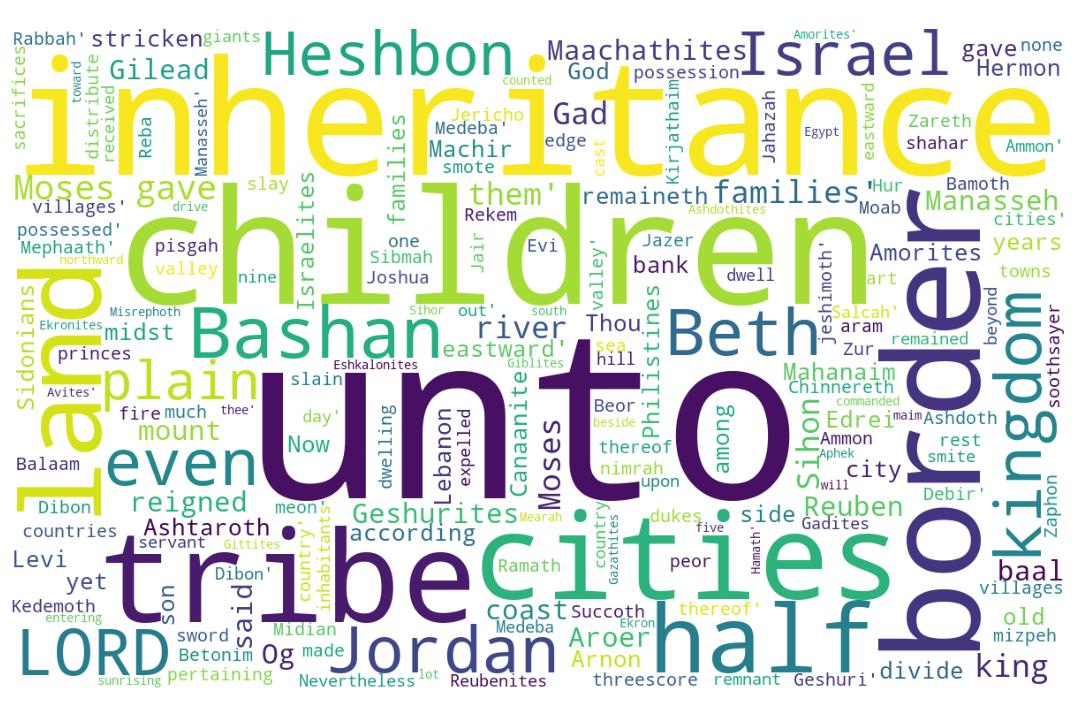
\includegraphics[width=\linewidth]{06OT-Joshua/Joshua13-WordCloud.jpg}
  \caption{Joshua 13 Word Cloud}
  \label{fig:Joshua 13 Word Cloud}
\end{figure}

\marginpar{\scriptsize \centering \fcolorbox{bone}{lime}{\textbf{FINISH THE JOB}}\\ (Joshua 13) \begin{compactenum}[I.][8]
	\item A \textbf{Duty} (to conquer and possess) \index[scripture]{Joshua!Jsh 13:02}  (Jsh 13:2) 
	\item The \textbf{Driving Out} (by God) \index[scripture]{Joshua!Jsh 13:06}  (Jsh 13:6) 
	\item The original \textbf{Divide} and Conquer  \index[scripture]{Joshua!Jsh 13:07}  (Jsh 13:7) 
	\item The \textbf{Distribution} to Rueben \index[scripture]{Joshua!Jsh 13:15--23}  (Jsh 13:15--23) 
	\item The \textbf{Dukes} \index[scripture]{Joshua!Jsh 13:21}  (Jsh 13:21) 
	\item The \textbf{Dwellingplaces} \index[scripture]{Joshua!Jsh 13:21}  (Jsh 13:21) 
	\item A \textbf{Distinct} Place \index[scripture]{Joshua!Jsh 13:33}  (Jsh 13:33) 
\end{compactenum}}




\footnote{\textcolor[rgb]{0.00,0.25,0.00}{\hyperlink{TOC}{Return to end of Table of Contents.}}}\footnote{\href{https://audiobible.com/bible/joshua_13.html}{\textcolor[cmyk]{0.99998,1,0,0}{Joshua 13 Audio}}}\textcolor[cmyk]{0.99998,1,0,0}{Now Joshua was old \emph{and} stricken in years; and the LORD said unto him, Thou art old \emph{and} stricken in years, and there remaineth yet very much land to be possessed.}
[2] \textcolor[cmyk]{0.99998,1,0,0}{This \emph{is} the land that yet remaineth: all the borders of the Philistines, and all Geshuri,}
[3] \textcolor[cmyk]{0.99998,1,0,0}{From Sihor, which \emph{is} before Egypt, even unto the borders of Ekron northward, \emph{which} is counted to the Canaanite: five lords of the Philistines; the Gazathites, and the Ashdothites, the Eshkalonites, the Gittites, and the Ekronites; also the Avites:}
[4] \textcolor[cmyk]{0.99998,1,0,0}{From the south, all the land of the Canaanites, and Mearah that \emph{is} beside the Sidonians, unto Aphek, to the borders of the Amorites:}
[5] \textcolor[cmyk]{0.99998,1,0,0}{And the land of the Giblites, and all Lebanon, toward the sunrising, from Baal-gad under mount Hermon unto the entering into Hamath.}
[6] \textcolor[cmyk]{0.99998,1,0,0}{All the inhabitants of the hill country from Lebanon unto Misrephoth-maim, \emph{and} all the Sidonians, them will I drive out from before  \fcolorbox{bone}{bone}{the children of} Israel: only divide thou it by lot unto the Israelites for an inheritance, as I have commanded thee.}
[7] \textcolor[cmyk]{0.99998,1,0,0}{Now therefore divide this land for an inheritance unto the nine tribes, and the half tribe of Manasseh,}
[8] \textcolor[cmyk]{0.99998,1,0,0}{With whom the Reubenites and the Gadites have received  \fcolorbox{bone}{bone}{their} inheritance, which Moses gave them, beyond Jordan eastward, \emph{even} as Moses the servant of the LORD gave them;}
[9] \textcolor[cmyk]{0.99998,1,0,0}{From Aroer, that \emph{is} upon the bank of the river Arnon, and the city that \emph{is} in the midst of the river, and all the plain of Medeba unto Dibon;}
[10] \textcolor[cmyk]{0.99998,1,0,0}{And all the cities of Sihon king of the Amorites, which reigned in Heshbon, unto the border of  \fcolorbox{bone}{bone}{the children of} Ammon;}
[11] \textcolor[cmyk]{0.99998,1,0,0}{And Gilead, and the border of the Geshurites and Maachathites, and all mount Hermon, and all Bashan unto Salcah;}
[12] \textcolor[cmyk]{0.99998,1,0,0}{All the kingdom of Og in Bashan, which reigned in Ashtaroth and in Edrei, who remained of the remnant of the giants: for these did Moses smite, and cast them out.}
[13] \textcolor[cmyk]{0.99998,1,0,0}{Nevertheless  \fcolorbox{bone}{bone}{the children of} Israel expelled not the Geshurites, nor the Maachathites: but the Geshurites and the Maachathites dwell among the Israelites until this day.}
[14] \textcolor[cmyk]{0.99998,1,0,0}{Only unto the tribe of Levi he gave none inheritance; the sacrifices of the LORD God of Israel made by fire \emph{are}  \fcolorbox{bone}{bone}{their} inheritance, as he said unto them.}\\
\\
\P  \textcolor[cmyk]{0.99998,1,0,0}{And Moses gave unto the tribe of  \fcolorbox{bone}{bone}{the children of} Reuben \emph{inheritance} according to  \fcolorbox{bone}{bone}{their} families.}
[16] \textcolor[cmyk]{0.99998,1,0,0}{And  \fcolorbox{bone}{bone}{their} coast was from Aroer, that \emph{is} on the bank of the river Arnon, and the city that \emph{is} in the midst of the river, and all the plain by Medeba;}
[17] \textcolor[cmyk]{0.99998,1,0,0}{Heshbon, and all her cities that \emph{are} in the plain; Dibon, and Bamoth-baal, and Beth-baal-meon,}
[18] \textcolor[cmyk]{0.99998,1,0,0}{And Jahazah, and Kedemoth, and Mephaath,}
[19] \textcolor[cmyk]{0.99998,1,0,0}{And Kirjathaim, and Sibmah, and \fcolorbox{bone}{MYGOLD}{Zareth-shahar} in the mount of the valley,}
[20] \textcolor[cmyk]{0.99998,1,0,0}{And Beth-peor, and Ashdoth-pisgah, and Beth-jeshimoth,}
[21] \textcolor[cmyk]{0.99998,1,0,0}{And all the cities of the plain, and all the kingdom of Sihon king of the Amorites, which reigned in Heshbon, whom Moses smote with the princes of Midian, Evi, and Rekem, and Zur, and Hur, and Reba, \emph{which} \emph{were} dukes of Sihon, dwelling in the country.}\\
\\
\P  \textcolor[cmyk]{0.99998,1,0,0}{Balaam also the son of Beor, the soothsayer, did  \fcolorbox{bone}{bone}{the children of} Israel slay with the sword among them that were slain by them.}
[23] \textcolor[cmyk]{0.99998,1,0,0}{And the border of  \fcolorbox{bone}{bone}{the children of} Reuben was Jordan, and the border \emph{thereof}. This \emph{was} the inheritance of  \fcolorbox{bone}{bone}{the children} \fcolorbox{bone}{bone}{of} Reuben after  \fcolorbox{bone}{bone}{their} families, the cities and the villages thereof.}
[24] \textcolor[cmyk]{0.99998,1,0,0}{And Moses gave \emph{inheritance} unto the tribe of Gad, \emph{even} unto  \fcolorbox{bone}{bone}{the children of} Gad according to  \fcolorbox{bone}{bone}{their} families.}
[25] \textcolor[cmyk]{0.99998,1,0,0}{And  \fcolorbox{bone}{bone}{their} coast was Jazer, and all the cities of Gilead, and half the land of  \fcolorbox{bone}{bone}{the children of} Ammon, unto Aroer that \emph{is} before Rabbah;}\
[26] \textcolor[cmyk]{0.99998,1,0,0}{And from Heshbon unto \fcolorbox{bone}{MYGOLD}{Ramath-mizpeh}, and Betonim; and from Mahanaim unto the border of Debir;}
[27] \textcolor[cmyk]{0.99998,1,0,0}{And in the valley, Beth-aram, and Beth-nimrah, and Succoth, and Zaphon, the rest of the kingdom of Sihon king of Heshbon, Jordan and \emph{his} border, \emph{even} unto the edge of the sea of Chinnereth on the other side Jordan eastward.}
[28] \textcolor[cmyk]{0.99998,1,0,0}{This \emph{is} the inheritance of  \fcolorbox{bone}{bone}{the children of} Gad after  \fcolorbox{bone}{bone}{their} families, the cities, and  \fcolorbox{bone}{bone}{their} villages.}\\
\\
\P \textcolor[cmyk]{0.99998,1,0,0}{And Moses gave \emph{inheritance} unto the half tribe of Manasseh: and \emph{this} was \emph{the} \emph{possession} of the half tribe of  \fcolorbox{bone}{bone}{the children of} Manasseh by  \fcolorbox{bone}{bone}{their} families.}
[30] \textcolor[cmyk]{0.99998,1,0,0}{And  \fcolorbox{bone}{bone}{their} coast was from Mahanaim, all Bashan, all the kingdom of Og king of Bashan, and all the towns of Jair, which \emph{are} in Bashan, threescore cities:}
[31] \textcolor[cmyk]{0.99998,1,0,0}{And half Gilead, and Ashtaroth, and Edrei, cities of the kingdom of Og in Bashan, \emph{were} \emph{pertaining} unto  \fcolorbox{bone}{bone}{the children of} Machir the son of Manasseh, \emph{even} to the one half of  \fcolorbox{bone}{bone}{the children of} Machir by  \fcolorbox{bone}{bone}{their} families.}
[32] \textcolor[cmyk]{0.99998,1,0,0}{These \emph{are} \emph{the} \emph{countries} which Moses did distribute for inheritance in the plains of Moab, on the other side Jordan, by Jericho, eastward.}
[33] \textcolor[cmyk]{0.99998,1,0,0}{But unto the tribe of Levi Moses gave not \emph{any} inheritance: the LORD God of Israel \emph{was}  \fcolorbox{bone}{bone}{their} inheritance, as he said unto them.}

\index[NWIV]{31!Joshua!Jos 13:1}\index[AWIP]{Now!Joshua!Jos 13:1}\index[AWIP]{Joshua!Joshua!Jos 13:1}\index[AWIP]{was!Joshua!Jos 13:1}\index[AWIP]{old!Joshua!Jos 13:1}\index[AWIP]{old!Joshua!Jos 13:1 (2)}\index[AWIP]{\emph{and}!Joshua!Jos 13:1}\index[AWIP]{\emph{and}!Joshua!Jos 13:1 (2)}\index[AWIP]{stricken!Joshua!Jos 13:1}\index[AWIP]{stricken!Joshua!Jos 13:1 (2)}\index[AWIP]{in!Joshua!Jos 13:1}\index[AWIP]{in!Joshua!Jos 13:1 (2)}\index[AWIP]{years!Joshua!Jos 13:1}\index[AWIP]{years!Joshua!Jos 13:1 (2)}\index[AWIP]{and!Joshua!Jos 13:1}\index[AWIP]{and!Joshua!Jos 13:1 (2)}\index[AWIP]{the!Joshua!Jos 13:1}\index[AWIP]{LORD!Joshua!Jos 13:1}\index[AWIP]{said!Joshua!Jos 13:1}\index[AWIP]{unto!Joshua!Jos 13:1}\index[AWIP]{him!Joshua!Jos 13:1}\index[AWIP]{Thou!Joshua!Jos 13:1}\index[AWIP]{art!Joshua!Jos 13:1}\index[AWIP]{there!Joshua!Jos 13:1}\index[AWIP]{remaineth!Joshua!Jos 13:1}\index[AWIP]{yet!Joshua!Jos 13:1}\index[AWIP]{very!Joshua!Jos 13:1}\index[AWIP]{much!Joshua!Jos 13:1}\index[AWIP]{land!Joshua!Jos 13:1}\index[AWIP]{to!Joshua!Jos 13:1}\index[AWIP]{be!Joshua!Jos 13:1}\index[AWIP]{possessed!Joshua!Jos 13:1}\index[AWIP]{\emph{and}!Joshua!Jos 13:1}\index[AWIP]{\emph{and}!Joshua!Jos 13:1 (2)}

\index[NWIV]{16!Joshua!Jos 13:2}\index[AWIP]{This!Joshua!Jos 13:2}\index[AWIP]{\emph{is}!Joshua!Jos 13:2}\index[AWIP]{the!Joshua!Jos 13:2}\index[AWIP]{the!Joshua!Jos 13:2 (2)}\index[AWIP]{the!Joshua!Jos 13:2 (3)}\index[AWIP]{land!Joshua!Jos 13:2}\index[AWIP]{that!Joshua!Jos 13:2}\index[AWIP]{yet!Joshua!Jos 13:2}\index[AWIP]{remaineth!Joshua!Jos 13:2}\index[AWIP]{all!Joshua!Jos 13:2}\index[AWIP]{all!Joshua!Jos 13:2 (2)}\index[AWIP]{borders!Joshua!Jos 13:2}\index[AWIP]{of!Joshua!Jos 13:2}\index[AWIP]{Philistines!Joshua!Jos 13:2}\index[AWIP]{and!Joshua!Jos 13:2}\index[AWIP]{Geshuri!Joshua!Jos 13:2}\index[AWIP]{\emph{is}!Joshua!Jos 13:2}

\index[NWIV]{39!Joshua!Jos 13:3}\index[AWIP]{From!Joshua!Jos 13:3}\index[AWIP]{Sihor!Joshua!Jos 13:3}\index[AWIP]{which!Joshua!Jos 13:3}\index[AWIP]{\emph{is}!Joshua!Jos 13:3}\index[AWIP]{before!Joshua!Jos 13:3}\index[AWIP]{Egypt!Joshua!Jos 13:3}\index[AWIP]{even!Joshua!Jos 13:3}\index[AWIP]{unto!Joshua!Jos 13:3}\index[AWIP]{the!Joshua!Jos 13:3}\index[AWIP]{the!Joshua!Jos 13:3 (2)}\index[AWIP]{the!Joshua!Jos 13:3 (3)}\index[AWIP]{the!Joshua!Jos 13:3 (4)}\index[AWIP]{the!Joshua!Jos 13:3 (5)}\index[AWIP]{the!Joshua!Jos 13:3 (6)}\index[AWIP]{the!Joshua!Jos 13:3 (7)}\index[AWIP]{the!Joshua!Jos 13:3 (8)}\index[AWIP]{the!Joshua!Jos 13:3 (9)}\index[AWIP]{borders!Joshua!Jos 13:3}\index[AWIP]{of!Joshua!Jos 13:3}\index[AWIP]{of!Joshua!Jos 13:3 (2)}\index[AWIP]{Ekron!Joshua!Jos 13:3}\index[AWIP]{northward!Joshua!Jos 13:3}\index[AWIP]{\emph{which}!Joshua!Jos 13:3}\index[AWIP]{is!Joshua!Jos 13:3}\index[AWIP]{counted!Joshua!Jos 13:3}\index[AWIP]{to!Joshua!Jos 13:3}\index[AWIP]{Canaanite!Joshua!Jos 13:3}\index[AWIP]{five!Joshua!Jos 13:3}\index[AWIP]{lords!Joshua!Jos 13:3}\index[AWIP]{Philistines!Joshua!Jos 13:3}\index[AWIP]{Gazathites!Joshua!Jos 13:3}\index[AWIP]{and!Joshua!Jos 13:3}\index[AWIP]{and!Joshua!Jos 13:3 (2)}\index[AWIP]{Ashdothites!Joshua!Jos 13:3}\index[AWIP]{Eshkalonites!Joshua!Jos 13:3}\index[AWIP]{Gittites!Joshua!Jos 13:3}\index[AWIP]{Ekronites!Joshua!Jos 13:3}\index[AWIP]{also!Joshua!Jos 13:3}\index[AWIP]{Avites!Joshua!Jos 13:3}\index[AWIP]{\emph{is}!Joshua!Jos 13:3}\index[AWIP]{\emph{which}!Joshua!Jos 13:3}

\index[NWIV]{24!Joshua!Jos 13:4}\index[AWIP]{From!Joshua!Jos 13:4}\index[AWIP]{the!Joshua!Jos 13:4}\index[AWIP]{the!Joshua!Jos 13:4 (2)}\index[AWIP]{the!Joshua!Jos 13:4 (3)}\index[AWIP]{the!Joshua!Jos 13:4 (4)}\index[AWIP]{the!Joshua!Jos 13:4 (5)}\index[AWIP]{the!Joshua!Jos 13:4 (6)}\index[AWIP]{south!Joshua!Jos 13:4}\index[AWIP]{all!Joshua!Jos 13:4}\index[AWIP]{land!Joshua!Jos 13:4}\index[AWIP]{of!Joshua!Jos 13:4}\index[AWIP]{of!Joshua!Jos 13:4 (2)}\index[AWIP]{Canaanites!Joshua!Jos 13:4}\index[AWIP]{and!Joshua!Jos 13:4}\index[AWIP]{Mearah!Joshua!Jos 13:4}\index[AWIP]{that!Joshua!Jos 13:4}\index[AWIP]{\emph{is}!Joshua!Jos 13:4}\index[AWIP]{beside!Joshua!Jos 13:4}\index[AWIP]{Sidonians!Joshua!Jos 13:4}\index[AWIP]{unto!Joshua!Jos 13:4}\index[AWIP]{Aphek!Joshua!Jos 13:4}\index[AWIP]{to!Joshua!Jos 13:4}\index[AWIP]{borders!Joshua!Jos 13:4}\index[AWIP]{Amorites!Joshua!Jos 13:4}\index[AWIP]{\emph{is}!Joshua!Jos 13:4}

\index[NWIV]{22!Joshua!Jos 13:5}\index[AWIP]{And!Joshua!Jos 13:5}\index[AWIP]{the!Joshua!Jos 13:5}\index[AWIP]{the!Joshua!Jos 13:5 (2)}\index[AWIP]{the!Joshua!Jos 13:5 (3)}\index[AWIP]{the!Joshua!Jos 13:5 (4)}\index[AWIP]{land!Joshua!Jos 13:5}\index[AWIP]{of!Joshua!Jos 13:5}\index[AWIP]{Giblites!Joshua!Jos 13:5}\index[AWIP]{and!Joshua!Jos 13:5}\index[AWIP]{all!Joshua!Jos 13:5}\index[AWIP]{Lebanon!Joshua!Jos 13:5}\index[AWIP]{toward!Joshua!Jos 13:5}\index[AWIP]{sunrising!Joshua!Jos 13:5}\index[AWIP]{from!Joshua!Jos 13:5}\index[AWIP]{Baal-gad!Joshua!Jos 13:5}\index[AWIP]{under!Joshua!Jos 13:5}\index[AWIP]{mount!Joshua!Jos 13:5}\index[AWIP]{Hermon!Joshua!Jos 13:5}\index[AWIP]{unto!Joshua!Jos 13:5}\index[AWIP]{entering!Joshua!Jos 13:5}\index[AWIP]{into!Joshua!Jos 13:5}\index[AWIP]{Hamath!Joshua!Jos 13:5}

\index[NWIV]{43!Joshua!Jos 13:6}\index[AWIP]{All!Joshua!Jos 13:6}\index[AWIP]{the!Joshua!Jos 13:6}\index[AWIP]{the!Joshua!Jos 13:6 (2)}\index[AWIP]{the!Joshua!Jos 13:6 (3)}\index[AWIP]{the!Joshua!Jos 13:6 (4)}\index[AWIP]{the!Joshua!Jos 13:6 (5)}\index[AWIP]{inhabitants!Joshua!Jos 13:6}\index[AWIP]{of!Joshua!Jos 13:6}\index[AWIP]{of!Joshua!Jos 13:6 (2)}\index[AWIP]{hill!Joshua!Jos 13:6}\index[AWIP]{country!Joshua!Jos 13:6}\index[AWIP]{from!Joshua!Jos 13:6}\index[AWIP]{from!Joshua!Jos 13:6 (2)}\index[AWIP]{Lebanon!Joshua!Jos 13:6}\index[AWIP]{unto!Joshua!Jos 13:6}\index[AWIP]{unto!Joshua!Jos 13:6 (2)}\index[AWIP]{Misrephoth-maim!Joshua!Jos 13:6}\index[AWIP]{\emph{and}!Joshua!Jos 13:6}\index[AWIP]{all!Joshua!Jos 13:6}\index[AWIP]{Sidonians!Joshua!Jos 13:6}\index[AWIP]{them!Joshua!Jos 13:6}\index[AWIP]{will!Joshua!Jos 13:6}\index[AWIP]{I!Joshua!Jos 13:6}\index[AWIP]{I!Joshua!Jos 13:6 (2)}\index[AWIP]{drive!Joshua!Jos 13:6}\index[AWIP]{out!Joshua!Jos 13:6}\index[AWIP]{before!Joshua!Jos 13:6}\index[AWIP]{children!Joshua!Jos 13:6}\index[AWIP]{Israel!Joshua!Jos 13:6}\index[AWIP]{only!Joshua!Jos 13:6}\index[AWIP]{divide!Joshua!Jos 13:6}\index[AWIP]{thou!Joshua!Jos 13:6}\index[AWIP]{it!Joshua!Jos 13:6}\index[AWIP]{by!Joshua!Jos 13:6}\index[AWIP]{lot!Joshua!Jos 13:6}\index[AWIP]{Israelites!Joshua!Jos 13:6}\index[AWIP]{for!Joshua!Jos 13:6}\index[AWIP]{an!Joshua!Jos 13:6}\index[AWIP]{inheritance!Joshua!Jos 13:6}\index[AWIP]{as!Joshua!Jos 13:6}\index[AWIP]{have!Joshua!Jos 13:6}\index[AWIP]{commanded!Joshua!Jos 13:6}\index[AWIP]{thee!Joshua!Jos 13:6}\index[AWIP]{\emph{and}!Joshua!Jos 13:6}

\index[NWIV]{18!Joshua!Jos 13:7}\index[AWIP]{Now!Joshua!Jos 13:7}\index[AWIP]{therefore!Joshua!Jos 13:7}\index[AWIP]{divide!Joshua!Jos 13:7}\index[AWIP]{this!Joshua!Jos 13:7}\index[AWIP]{land!Joshua!Jos 13:7}\index[AWIP]{for!Joshua!Jos 13:7}\index[AWIP]{an!Joshua!Jos 13:7}\index[AWIP]{inheritance!Joshua!Jos 13:7}\index[AWIP]{unto!Joshua!Jos 13:7}\index[AWIP]{the!Joshua!Jos 13:7}\index[AWIP]{the!Joshua!Jos 13:7 (2)}\index[AWIP]{nine!Joshua!Jos 13:7}\index[AWIP]{tribes!Joshua!Jos 13:7}\index[AWIP]{and!Joshua!Jos 13:7}\index[AWIP]{half!Joshua!Jos 13:7}\index[AWIP]{tribe!Joshua!Jos 13:7}\index[AWIP]{of!Joshua!Jos 13:7}\index[AWIP]{Manasseh!Joshua!Jos 13:7}

\index[NWIV]{28!Joshua!Jos 13:8}\index[AWIP]{With!Joshua!Jos 13:8}\index[AWIP]{whom!Joshua!Jos 13:8}\index[AWIP]{the!Joshua!Jos 13:8}\index[AWIP]{the!Joshua!Jos 13:8 (2)}\index[AWIP]{the!Joshua!Jos 13:8 (3)}\index[AWIP]{the!Joshua!Jos 13:8 (4)}\index[AWIP]{Reubenites!Joshua!Jos 13:8}\index[AWIP]{and!Joshua!Jos 13:8}\index[AWIP]{Gadites!Joshua!Jos 13:8}\index[AWIP]{have!Joshua!Jos 13:8}\index[AWIP]{received!Joshua!Jos 13:8}\index[AWIP]{their!Joshua!Jos 13:8}\index[AWIP]{inheritance!Joshua!Jos 13:8}\index[AWIP]{which!Joshua!Jos 13:8}\index[AWIP]{Moses!Joshua!Jos 13:8}\index[AWIP]{Moses!Joshua!Jos 13:8 (2)}\index[AWIP]{gave!Joshua!Jos 13:8}\index[AWIP]{gave!Joshua!Jos 13:8 (2)}\index[AWIP]{them!Joshua!Jos 13:8}\index[AWIP]{them!Joshua!Jos 13:8 (2)}\index[AWIP]{beyond!Joshua!Jos 13:8}\index[AWIP]{Jordan!Joshua!Jos 13:8}\index[AWIP]{eastward!Joshua!Jos 13:8}\index[AWIP]{\emph{even}!Joshua!Jos 13:8}\index[AWIP]{as!Joshua!Jos 13:8}\index[AWIP]{servant!Joshua!Jos 13:8}\index[AWIP]{of!Joshua!Jos 13:8}\index[AWIP]{LORD!Joshua!Jos 13:8}\index[AWIP]{\emph{even}!Joshua!Jos 13:8}

\index[NWIV]{30!Joshua!Jos 13:9}\index[AWIP]{From!Joshua!Jos 13:9}\index[AWIP]{Aroer!Joshua!Jos 13:9}\index[AWIP]{that!Joshua!Jos 13:9}\index[AWIP]{that!Joshua!Jos 13:9 (2)}\index[AWIP]{\emph{is}!Joshua!Jos 13:9}\index[AWIP]{\emph{is}!Joshua!Jos 13:9 (2)}\index[AWIP]{upon!Joshua!Jos 13:9}\index[AWIP]{the!Joshua!Jos 13:9}\index[AWIP]{the!Joshua!Jos 13:9 (2)}\index[AWIP]{the!Joshua!Jos 13:9 (3)}\index[AWIP]{the!Joshua!Jos 13:9 (4)}\index[AWIP]{the!Joshua!Jos 13:9 (5)}\index[AWIP]{the!Joshua!Jos 13:9 (6)}\index[AWIP]{bank!Joshua!Jos 13:9}\index[AWIP]{of!Joshua!Jos 13:9}\index[AWIP]{of!Joshua!Jos 13:9 (2)}\index[AWIP]{of!Joshua!Jos 13:9 (3)}\index[AWIP]{river!Joshua!Jos 13:9}\index[AWIP]{river!Joshua!Jos 13:9 (2)}\index[AWIP]{Arnon!Joshua!Jos 13:9}\index[AWIP]{and!Joshua!Jos 13:9}\index[AWIP]{and!Joshua!Jos 13:9 (2)}\index[AWIP]{city!Joshua!Jos 13:9}\index[AWIP]{in!Joshua!Jos 13:9}\index[AWIP]{midst!Joshua!Jos 13:9}\index[AWIP]{all!Joshua!Jos 13:9}\index[AWIP]{plain!Joshua!Jos 13:9}\index[AWIP]{Medeba!Joshua!Jos 13:9}\index[AWIP]{unto!Joshua!Jos 13:9}\index[AWIP]{Dibon!Joshua!Jos 13:9}\index[AWIP]{\emph{is}!Joshua!Jos 13:9}\index[AWIP]{\emph{is}!Joshua!Jos 13:9 (2)}

\index[NWIV]{22!Joshua!Jos 13:10}\index[AWIP]{And!Joshua!Jos 13:10}\index[AWIP]{all!Joshua!Jos 13:10}\index[AWIP]{the!Joshua!Jos 13:10}\index[AWIP]{the!Joshua!Jos 13:10 (2)}\index[AWIP]{the!Joshua!Jos 13:10 (3)}\index[AWIP]{the!Joshua!Jos 13:10 (4)}\index[AWIP]{cities!Joshua!Jos 13:10}\index[AWIP]{of!Joshua!Jos 13:10}\index[AWIP]{of!Joshua!Jos 13:10 (2)}\index[AWIP]{of!Joshua!Jos 13:10 (3)}\index[AWIP]{of!Joshua!Jos 13:10 (4)}\index[AWIP]{Sihon!Joshua!Jos 13:10}\index[AWIP]{king!Joshua!Jos 13:10}\index[AWIP]{Amorites!Joshua!Jos 13:10}\index[AWIP]{which!Joshua!Jos 13:10}\index[AWIP]{reigned!Joshua!Jos 13:10}\index[AWIP]{in!Joshua!Jos 13:10}\index[AWIP]{Heshbon!Joshua!Jos 13:10}\index[AWIP]{unto!Joshua!Jos 13:10}\index[AWIP]{border!Joshua!Jos 13:10}\index[AWIP]{children!Joshua!Jos 13:10}\index[AWIP]{Ammon!Joshua!Jos 13:10}

\index[NWIV]{19!Joshua!Jos 13:11}\index[AWIP]{And!Joshua!Jos 13:11}\index[AWIP]{Gilead!Joshua!Jos 13:11}\index[AWIP]{and!Joshua!Jos 13:11}\index[AWIP]{and!Joshua!Jos 13:11 (2)}\index[AWIP]{and!Joshua!Jos 13:11 (3)}\index[AWIP]{and!Joshua!Jos 13:11 (4)}\index[AWIP]{the!Joshua!Jos 13:11}\index[AWIP]{the!Joshua!Jos 13:11 (2)}\index[AWIP]{border!Joshua!Jos 13:11}\index[AWIP]{of!Joshua!Jos 13:11}\index[AWIP]{Geshurites!Joshua!Jos 13:11}\index[AWIP]{Maachathites!Joshua!Jos 13:11}\index[AWIP]{all!Joshua!Jos 13:11}\index[AWIP]{all!Joshua!Jos 13:11 (2)}\index[AWIP]{mount!Joshua!Jos 13:11}\index[AWIP]{Hermon!Joshua!Jos 13:11}\index[AWIP]{Bashan!Joshua!Jos 13:11}\index[AWIP]{unto!Joshua!Jos 13:11}\index[AWIP]{Salcah!Joshua!Jos 13:11}

\index[NWIV]{31!Joshua!Jos 13:12}\index[AWIP]{All!Joshua!Jos 13:12}\index[AWIP]{the!Joshua!Jos 13:12}\index[AWIP]{the!Joshua!Jos 13:12 (2)}\index[AWIP]{the!Joshua!Jos 13:12 (3)}\index[AWIP]{kingdom!Joshua!Jos 13:12}\index[AWIP]{of!Joshua!Jos 13:12}\index[AWIP]{of!Joshua!Jos 13:12 (2)}\index[AWIP]{of!Joshua!Jos 13:12 (3)}\index[AWIP]{Og!Joshua!Jos 13:12}\index[AWIP]{in!Joshua!Jos 13:12}\index[AWIP]{in!Joshua!Jos 13:12 (2)}\index[AWIP]{in!Joshua!Jos 13:12 (3)}\index[AWIP]{Bashan!Joshua!Jos 13:12}\index[AWIP]{which!Joshua!Jos 13:12}\index[AWIP]{reigned!Joshua!Jos 13:12}\index[AWIP]{Ashtaroth!Joshua!Jos 13:12}\index[AWIP]{and!Joshua!Jos 13:12}\index[AWIP]{and!Joshua!Jos 13:12 (2)}\index[AWIP]{Edrei!Joshua!Jos 13:12}\index[AWIP]{who!Joshua!Jos 13:12}\index[AWIP]{remained!Joshua!Jos 13:12}\index[AWIP]{remnant!Joshua!Jos 13:12}\index[AWIP]{giants!Joshua!Jos 13:12}\index[AWIP]{for!Joshua!Jos 13:12}\index[AWIP]{these!Joshua!Jos 13:12}\index[AWIP]{did!Joshua!Jos 13:12}\index[AWIP]{Moses!Joshua!Jos 13:12}\index[AWIP]{smite!Joshua!Jos 13:12}\index[AWIP]{cast!Joshua!Jos 13:12}\index[AWIP]{them!Joshua!Jos 13:12}\index[AWIP]{out!Joshua!Jos 13:12}

\index[NWIV]{25!Joshua!Jos 13:13}\index[AWIP]{Nevertheless!Joshua!Jos 13:13}\index[AWIP]{the!Joshua!Jos 13:13}\index[AWIP]{the!Joshua!Jos 13:13 (2)}\index[AWIP]{the!Joshua!Jos 13:13 (3)}\index[AWIP]{the!Joshua!Jos 13:13 (4)}\index[AWIP]{the!Joshua!Jos 13:13 (5)}\index[AWIP]{the!Joshua!Jos 13:13 (6)}\index[AWIP]{children!Joshua!Jos 13:13}\index[AWIP]{of!Joshua!Jos 13:13}\index[AWIP]{Israel!Joshua!Jos 13:13}\index[AWIP]{expelled!Joshua!Jos 13:13}\index[AWIP]{not!Joshua!Jos 13:13}\index[AWIP]{Geshurites!Joshua!Jos 13:13}\index[AWIP]{Geshurites!Joshua!Jos 13:13 (2)}\index[AWIP]{nor!Joshua!Jos 13:13}\index[AWIP]{Maachathites!Joshua!Jos 13:13}\index[AWIP]{Maachathites!Joshua!Jos 13:13 (2)}\index[AWIP]{but!Joshua!Jos 13:13}\index[AWIP]{and!Joshua!Jos 13:13}\index[AWIP]{dwell!Joshua!Jos 13:13}\index[AWIP]{among!Joshua!Jos 13:13}\index[AWIP]{Israelites!Joshua!Jos 13:13}\index[AWIP]{until!Joshua!Jos 13:13}\index[AWIP]{this!Joshua!Jos 13:13}\index[AWIP]{day!Joshua!Jos 13:13}

\index[NWIV]{29!Joshua!Jos 13:14}\index[AWIP]{Only!Joshua!Jos 13:14}\index[AWIP]{unto!Joshua!Jos 13:14}\index[AWIP]{unto!Joshua!Jos 13:14 (2)}\index[AWIP]{the!Joshua!Jos 13:14}\index[AWIP]{the!Joshua!Jos 13:14 (2)}\index[AWIP]{the!Joshua!Jos 13:14 (3)}\index[AWIP]{tribe!Joshua!Jos 13:14}\index[AWIP]{of!Joshua!Jos 13:14}\index[AWIP]{of!Joshua!Jos 13:14 (2)}\index[AWIP]{of!Joshua!Jos 13:14 (3)}\index[AWIP]{Levi!Joshua!Jos 13:14}\index[AWIP]{he!Joshua!Jos 13:14}\index[AWIP]{he!Joshua!Jos 13:14 (2)}\index[AWIP]{gave!Joshua!Jos 13:14}\index[AWIP]{none!Joshua!Jos 13:14}\index[AWIP]{inheritance!Joshua!Jos 13:14}\index[AWIP]{inheritance!Joshua!Jos 13:14 (2)}\index[AWIP]{sacrifices!Joshua!Jos 13:14}\index[AWIP]{LORD!Joshua!Jos 13:14}\index[AWIP]{God!Joshua!Jos 13:14}\index[AWIP]{Israel!Joshua!Jos 13:14}\index[AWIP]{made!Joshua!Jos 13:14}\index[AWIP]{by!Joshua!Jos 13:14}\index[AWIP]{fire!Joshua!Jos 13:14}\index[AWIP]{\emph{are}!Joshua!Jos 13:14}\index[AWIP]{their!Joshua!Jos 13:14}\index[AWIP]{as!Joshua!Jos 13:14}\index[AWIP]{said!Joshua!Jos 13:14}\index[AWIP]{them!Joshua!Jos 13:14}\index[AWIP]{\emph{are}!Joshua!Jos 13:14}

\index[NWIV]{16!Joshua!Jos 13:15}\index[AWIP]{And!Joshua!Jos 13:15}\index[AWIP]{Moses!Joshua!Jos 13:15}\index[AWIP]{gave!Joshua!Jos 13:15}\index[AWIP]{unto!Joshua!Jos 13:15}\index[AWIP]{the!Joshua!Jos 13:15}\index[AWIP]{the!Joshua!Jos 13:15 (2)}\index[AWIP]{tribe!Joshua!Jos 13:15}\index[AWIP]{of!Joshua!Jos 13:15}\index[AWIP]{of!Joshua!Jos 13:15 (2)}\index[AWIP]{children!Joshua!Jos 13:15}\index[AWIP]{Reuben!Joshua!Jos 13:15}\index[AWIP]{\emph{inheritance}!Joshua!Jos 13:15}\index[AWIP]{according!Joshua!Jos 13:15}\index[AWIP]{to!Joshua!Jos 13:15}\index[AWIP]{their!Joshua!Jos 13:15}\index[AWIP]{families!Joshua!Jos 13:15}\index[AWIP]{\emph{inheritance}!Joshua!Jos 13:15}

\index[NWIV]{32!Joshua!Jos 13:16}\index[AWIP]{And!Joshua!Jos 13:16}\index[AWIP]{their!Joshua!Jos 13:16}\index[AWIP]{coast!Joshua!Jos 13:16}\index[AWIP]{was!Joshua!Jos 13:16}\index[AWIP]{from!Joshua!Jos 13:16}\index[AWIP]{Aroer!Joshua!Jos 13:16}\index[AWIP]{that!Joshua!Jos 13:16}\index[AWIP]{that!Joshua!Jos 13:16 (2)}\index[AWIP]{\emph{is}!Joshua!Jos 13:16}\index[AWIP]{\emph{is}!Joshua!Jos 13:16 (2)}\index[AWIP]{on!Joshua!Jos 13:16}\index[AWIP]{the!Joshua!Jos 13:16}\index[AWIP]{the!Joshua!Jos 13:16 (2)}\index[AWIP]{the!Joshua!Jos 13:16 (3)}\index[AWIP]{the!Joshua!Jos 13:16 (4)}\index[AWIP]{the!Joshua!Jos 13:16 (5)}\index[AWIP]{the!Joshua!Jos 13:16 (6)}\index[AWIP]{bank!Joshua!Jos 13:16}\index[AWIP]{of!Joshua!Jos 13:16}\index[AWIP]{of!Joshua!Jos 13:16 (2)}\index[AWIP]{river!Joshua!Jos 13:16}\index[AWIP]{river!Joshua!Jos 13:16 (2)}\index[AWIP]{Arnon!Joshua!Jos 13:16}\index[AWIP]{and!Joshua!Jos 13:16}\index[AWIP]{and!Joshua!Jos 13:16 (2)}\index[AWIP]{city!Joshua!Jos 13:16}\index[AWIP]{in!Joshua!Jos 13:16}\index[AWIP]{midst!Joshua!Jos 13:16}\index[AWIP]{all!Joshua!Jos 13:16}\index[AWIP]{plain!Joshua!Jos 13:16}\index[AWIP]{by!Joshua!Jos 13:16}\index[AWIP]{Medeba!Joshua!Jos 13:16}\index[AWIP]{\emph{is}!Joshua!Jos 13:16}\index[AWIP]{\emph{is}!Joshua!Jos 13:16 (2)}

\index[NWIV]{15!Joshua!Jos 13:17}\index[AWIP]{Heshbon!Joshua!Jos 13:17}\index[AWIP]{and!Joshua!Jos 13:17}\index[AWIP]{and!Joshua!Jos 13:17 (2)}\index[AWIP]{and!Joshua!Jos 13:17 (3)}\index[AWIP]{all!Joshua!Jos 13:17}\index[AWIP]{her!Joshua!Jos 13:17}\index[AWIP]{cities!Joshua!Jos 13:17}\index[AWIP]{that!Joshua!Jos 13:17}\index[AWIP]{\emph{are}!Joshua!Jos 13:17}\index[AWIP]{in!Joshua!Jos 13:17}\index[AWIP]{the!Joshua!Jos 13:17}\index[AWIP]{plain!Joshua!Jos 13:17}\index[AWIP]{Dibon!Joshua!Jos 13:17}\index[AWIP]{Bamoth-baal!Joshua!Jos 13:17}\index[AWIP]{Beth-baal-meon!Joshua!Jos 13:17}\index[AWIP]{\emph{are}!Joshua!Jos 13:17}

\index[NWIV]{6!Joshua!Jos 13:18}\index[AWIP]{And!Joshua!Jos 13:18}\index[AWIP]{Jahazah!Joshua!Jos 13:18}\index[AWIP]{and!Joshua!Jos 13:18}\index[AWIP]{and!Joshua!Jos 13:18 (2)}\index[AWIP]{Kedemoth!Joshua!Jos 13:18}\index[AWIP]{Mephaath!Joshua!Jos 13:18}

\index[NWIV]{12!Joshua!Jos 13:19}\index[AWIP]{And!Joshua!Jos 13:19}\index[AWIP]{Kirjathaim!Joshua!Jos 13:19}\index[AWIP]{and!Joshua!Jos 13:19}\index[AWIP]{and!Joshua!Jos 13:19 (2)}\index[AWIP]{Sibmah!Joshua!Jos 13:19}\index[AWIP]{Zareth-shahar!Joshua!Jos 13:19}\index[AWIP]{in!Joshua!Jos 13:19}\index[AWIP]{the!Joshua!Jos 13:19}\index[AWIP]{the!Joshua!Jos 13:19 (2)}\index[AWIP]{mount!Joshua!Jos 13:19}\index[AWIP]{of!Joshua!Jos 13:19}\index[AWIP]{valley!Joshua!Jos 13:19}

\index[NWIV]{6!Joshua!Jos 13:20}\index[AWIP]{And!Joshua!Jos 13:20}\index[AWIP]{Beth-peor!Joshua!Jos 13:20}\index[AWIP]{and!Joshua!Jos 13:20}\index[AWIP]{and!Joshua!Jos 13:20 (2)}\index[AWIP]{Ashdoth-pisgah!Joshua!Jos 13:20}\index[AWIP]{Beth-jeshimoth!Joshua!Jos 13:20}

\index[NWIV]{47!Joshua!Jos 13:21}\index[AWIP]{And!Joshua!Jos 13:21}\index[AWIP]{all!Joshua!Jos 13:21}\index[AWIP]{all!Joshua!Jos 13:21 (2)}\index[AWIP]{the!Joshua!Jos 13:21}\index[AWIP]{the!Joshua!Jos 13:21 (2)}\index[AWIP]{the!Joshua!Jos 13:21 (3)}\index[AWIP]{the!Joshua!Jos 13:21 (4)}\index[AWIP]{the!Joshua!Jos 13:21 (5)}\index[AWIP]{the!Joshua!Jos 13:21 (6)}\index[AWIP]{cities!Joshua!Jos 13:21}\index[AWIP]{of!Joshua!Jos 13:21}\index[AWIP]{of!Joshua!Jos 13:21 (2)}\index[AWIP]{of!Joshua!Jos 13:21 (3)}\index[AWIP]{of!Joshua!Jos 13:21 (4)}\index[AWIP]{of!Joshua!Jos 13:21 (5)}\index[AWIP]{plain!Joshua!Jos 13:21}\index[AWIP]{and!Joshua!Jos 13:21}\index[AWIP]{and!Joshua!Jos 13:21 (2)}\index[AWIP]{and!Joshua!Jos 13:21 (3)}\index[AWIP]{and!Joshua!Jos 13:21 (4)}\index[AWIP]{and!Joshua!Jos 13:21 (5)}\index[AWIP]{kingdom!Joshua!Jos 13:21}\index[AWIP]{Sihon!Joshua!Jos 13:21}\index[AWIP]{Sihon!Joshua!Jos 13:21 (2)}\index[AWIP]{king!Joshua!Jos 13:21}\index[AWIP]{Amorites!Joshua!Jos 13:21}\index[AWIP]{which!Joshua!Jos 13:21}\index[AWIP]{reigned!Joshua!Jos 13:21}\index[AWIP]{in!Joshua!Jos 13:21}\index[AWIP]{in!Joshua!Jos 13:21 (2)}\index[AWIP]{Heshbon!Joshua!Jos 13:21}\index[AWIP]{whom!Joshua!Jos 13:21}\index[AWIP]{Moses!Joshua!Jos 13:21}\index[AWIP]{smote!Joshua!Jos 13:21}\index[AWIP]{with!Joshua!Jos 13:21}\index[AWIP]{princes!Joshua!Jos 13:21}\index[AWIP]{Midian!Joshua!Jos 13:21}\index[AWIP]{Evi!Joshua!Jos 13:21}\index[AWIP]{Rekem!Joshua!Jos 13:21}\index[AWIP]{Zur!Joshua!Jos 13:21}\index[AWIP]{Hur!Joshua!Jos 13:21}\index[AWIP]{Reba!Joshua!Jos 13:21}\index[AWIP]{\emph{which}!Joshua!Jos 13:21}\index[AWIP]{\emph{were}!Joshua!Jos 13:21}\index[AWIP]{dukes!Joshua!Jos 13:21}\index[AWIP]{dwelling!Joshua!Jos 13:21}\index[AWIP]{country!Joshua!Jos 13:21}\index[AWIP]{\emph{which}!Joshua!Jos 13:21}\index[AWIP]{\emph{were}!Joshua!Jos 13:21}

\index[NWIV]{24!Joshua!Jos 13:22}\index[AWIP]{Balaam!Joshua!Jos 13:22}\index[AWIP]{also!Joshua!Jos 13:22}\index[AWIP]{the!Joshua!Jos 13:22}\index[AWIP]{the!Joshua!Jos 13:22 (2)}\index[AWIP]{the!Joshua!Jos 13:22 (3)}\index[AWIP]{the!Joshua!Jos 13:22 (4)}\index[AWIP]{son!Joshua!Jos 13:22}\index[AWIP]{of!Joshua!Jos 13:22}\index[AWIP]{of!Joshua!Jos 13:22 (2)}\index[AWIP]{Beor!Joshua!Jos 13:22}\index[AWIP]{soothsayer!Joshua!Jos 13:22}\index[AWIP]{did!Joshua!Jos 13:22}\index[AWIP]{children!Joshua!Jos 13:22}\index[AWIP]{Israel!Joshua!Jos 13:22}\index[AWIP]{slay!Joshua!Jos 13:22}\index[AWIP]{with!Joshua!Jos 13:22}\index[AWIP]{sword!Joshua!Jos 13:22}\index[AWIP]{among!Joshua!Jos 13:22}\index[AWIP]{them!Joshua!Jos 13:22}\index[AWIP]{them!Joshua!Jos 13:22 (2)}\index[AWIP]{that!Joshua!Jos 13:22}\index[AWIP]{were!Joshua!Jos 13:22}\index[AWIP]{slain!Joshua!Jos 13:22}\index[AWIP]{by!Joshua!Jos 13:22}

\index[NWIV]{32!Joshua!Jos 13:23}\index[AWIP]{And!Joshua!Jos 13:23}\index[AWIP]{the!Joshua!Jos 13:23}\index[AWIP]{the!Joshua!Jos 13:23 (2)}\index[AWIP]{the!Joshua!Jos 13:23 (3)}\index[AWIP]{the!Joshua!Jos 13:23 (4)}\index[AWIP]{the!Joshua!Jos 13:23 (5)}\index[AWIP]{the!Joshua!Jos 13:23 (6)}\index[AWIP]{the!Joshua!Jos 13:23 (7)}\index[AWIP]{border!Joshua!Jos 13:23}\index[AWIP]{border!Joshua!Jos 13:23 (2)}\index[AWIP]{of!Joshua!Jos 13:23}\index[AWIP]{of!Joshua!Jos 13:23 (2)}\index[AWIP]{of!Joshua!Jos 13:23 (3)}\index[AWIP]{of!Joshua!Jos 13:23 (4)}\index[AWIP]{children!Joshua!Jos 13:23}\index[AWIP]{children!Joshua!Jos 13:23 (2)}\index[AWIP]{Reuben!Joshua!Jos 13:23}\index[AWIP]{Reuben!Joshua!Jos 13:23 (2)}\index[AWIP]{was!Joshua!Jos 13:23}\index[AWIP]{Jordan!Joshua!Jos 13:23}\index[AWIP]{and!Joshua!Jos 13:23}\index[AWIP]{and!Joshua!Jos 13:23 (2)}\index[AWIP]{\emph{thereof}!Joshua!Jos 13:23}\index[AWIP]{This!Joshua!Jos 13:23}\index[AWIP]{\emph{was}!Joshua!Jos 13:23}\index[AWIP]{inheritance!Joshua!Jos 13:23}\index[AWIP]{after!Joshua!Jos 13:23}\index[AWIP]{their!Joshua!Jos 13:23}\index[AWIP]{families!Joshua!Jos 13:23}\index[AWIP]{cities!Joshua!Jos 13:23}\index[AWIP]{villages!Joshua!Jos 13:23}\index[AWIP]{thereof!Joshua!Jos 13:23}\index[AWIP]{\emph{thereof}!Joshua!Jos 13:23}\index[AWIP]{\emph{was}!Joshua!Jos 13:23}

\index[NWIV]{19!Joshua!Jos 13:24}\index[AWIP]{And!Joshua!Jos 13:24}\index[AWIP]{Moses!Joshua!Jos 13:24}\index[AWIP]{gave!Joshua!Jos 13:24}\index[AWIP]{\emph{inheritance}!Joshua!Jos 13:24}\index[AWIP]{unto!Joshua!Jos 13:24}\index[AWIP]{unto!Joshua!Jos 13:24 (2)}\index[AWIP]{the!Joshua!Jos 13:24}\index[AWIP]{the!Joshua!Jos 13:24 (2)}\index[AWIP]{tribe!Joshua!Jos 13:24}\index[AWIP]{of!Joshua!Jos 13:24}\index[AWIP]{of!Joshua!Jos 13:24 (2)}\index[AWIP]{Gad!Joshua!Jos 13:24}\index[AWIP]{Gad!Joshua!Jos 13:24 (2)}\index[AWIP]{\emph{even}!Joshua!Jos 13:24}\index[AWIP]{children!Joshua!Jos 13:24}\index[AWIP]{according!Joshua!Jos 13:24}\index[AWIP]{to!Joshua!Jos 13:24}\index[AWIP]{their!Joshua!Jos 13:24}\index[AWIP]{families!Joshua!Jos 13:24}\index[AWIP]{\emph{inheritance}!Joshua!Jos 13:24}\index[AWIP]{\emph{even}!Joshua!Jos 13:24}

\index[NWIV]{26!Joshua!Jos 13:25}\index[AWIP]{And!Joshua!Jos 13:25}\index[AWIP]{their!Joshua!Jos 13:25}\index[AWIP]{coast!Joshua!Jos 13:25}\index[AWIP]{was!Joshua!Jos 13:25}\index[AWIP]{Jazer!Joshua!Jos 13:25}\index[AWIP]{and!Joshua!Jos 13:25}\index[AWIP]{and!Joshua!Jos 13:25 (2)}\index[AWIP]{all!Joshua!Jos 13:25}\index[AWIP]{the!Joshua!Jos 13:25}\index[AWIP]{the!Joshua!Jos 13:25 (2)}\index[AWIP]{the!Joshua!Jos 13:25 (3)}\index[AWIP]{cities!Joshua!Jos 13:25}\index[AWIP]{of!Joshua!Jos 13:25}\index[AWIP]{of!Joshua!Jos 13:25 (2)}\index[AWIP]{of!Joshua!Jos 13:25 (3)}\index[AWIP]{Gilead!Joshua!Jos 13:25}\index[AWIP]{half!Joshua!Jos 13:25}\index[AWIP]{land!Joshua!Jos 13:25}\index[AWIP]{children!Joshua!Jos 13:25}\index[AWIP]{Ammon!Joshua!Jos 13:25}\index[AWIP]{unto!Joshua!Jos 13:25}\index[AWIP]{Aroer!Joshua!Jos 13:25}\index[AWIP]{that!Joshua!Jos 13:25}\index[AWIP]{\emph{is}!Joshua!Jos 13:25}\index[AWIP]{before!Joshua!Jos 13:25}\index[AWIP]{Rabbah!Joshua!Jos 13:25}\index[AWIP]{\emph{is}!Joshua!Jos 13:25}

\index[NWIV]{15!Joshua!Jos 13:26}\index[AWIP]{And!Joshua!Jos 13:26}\index[AWIP]{from!Joshua!Jos 13:26}\index[AWIP]{from!Joshua!Jos 13:26 (2)}\index[AWIP]{Heshbon!Joshua!Jos 13:26}\index[AWIP]{unto!Joshua!Jos 13:26}\index[AWIP]{unto!Joshua!Jos 13:26 (2)}\index[AWIP]{Ramath-mizpeh!Joshua!Jos 13:26}\index[AWIP]{and!Joshua!Jos 13:26}\index[AWIP]{and!Joshua!Jos 13:26 (2)}\index[AWIP]{Betonim!Joshua!Jos 13:26}\index[AWIP]{Mahanaim!Joshua!Jos 13:26}\index[AWIP]{the!Joshua!Jos 13:26}\index[AWIP]{border!Joshua!Jos 13:26}\index[AWIP]{of!Joshua!Jos 13:26}\index[AWIP]{Debir!Joshua!Jos 13:26}

\index[NWIV]{40!Joshua!Jos 13:27}\index[AWIP]{And!Joshua!Jos 13:27}\index[AWIP]{in!Joshua!Jos 13:27}\index[AWIP]{the!Joshua!Jos 13:27}\index[AWIP]{the!Joshua!Jos 13:27 (2)}\index[AWIP]{the!Joshua!Jos 13:27 (3)}\index[AWIP]{the!Joshua!Jos 13:27 (4)}\index[AWIP]{the!Joshua!Jos 13:27 (5)}\index[AWIP]{the!Joshua!Jos 13:27 (6)}\index[AWIP]{valley!Joshua!Jos 13:27}\index[AWIP]{Beth-aram!Joshua!Jos 13:27}\index[AWIP]{and!Joshua!Jos 13:27}\index[AWIP]{and!Joshua!Jos 13:27 (2)}\index[AWIP]{and!Joshua!Jos 13:27 (3)}\index[AWIP]{and!Joshua!Jos 13:27 (4)}\index[AWIP]{Beth-nimrah!Joshua!Jos 13:27}\index[AWIP]{Succoth!Joshua!Jos 13:27}\index[AWIP]{Zaphon!Joshua!Jos 13:27}\index[AWIP]{rest!Joshua!Jos 13:27}\index[AWIP]{of!Joshua!Jos 13:27}\index[AWIP]{of!Joshua!Jos 13:27 (2)}\index[AWIP]{of!Joshua!Jos 13:27 (3)}\index[AWIP]{of!Joshua!Jos 13:27 (4)}\index[AWIP]{of!Joshua!Jos 13:27 (5)}\index[AWIP]{kingdom!Joshua!Jos 13:27}\index[AWIP]{Sihon!Joshua!Jos 13:27}\index[AWIP]{king!Joshua!Jos 13:27}\index[AWIP]{Heshbon!Joshua!Jos 13:27}\index[AWIP]{Jordan!Joshua!Jos 13:27}\index[AWIP]{Jordan!Joshua!Jos 13:27 (2)}\index[AWIP]{\emph{his}!Joshua!Jos 13:27}\index[AWIP]{border!Joshua!Jos 13:27}\index[AWIP]{\emph{even}!Joshua!Jos 13:27}\index[AWIP]{unto!Joshua!Jos 13:27}\index[AWIP]{edge!Joshua!Jos 13:27}\index[AWIP]{sea!Joshua!Jos 13:27}\index[AWIP]{Chinnereth!Joshua!Jos 13:27}\index[AWIP]{on!Joshua!Jos 13:27}\index[AWIP]{other!Joshua!Jos 13:27}\index[AWIP]{side!Joshua!Jos 13:27}\index[AWIP]{eastward!Joshua!Jos 13:27}\index[AWIP]{\emph{his}!Joshua!Jos 13:27}\index[AWIP]{\emph{even}!Joshua!Jos 13:27}

\index[NWIV]{17!Joshua!Jos 13:28}\index[AWIP]{This!Joshua!Jos 13:28}\index[AWIP]{\emph{is}!Joshua!Jos 13:28}\index[AWIP]{the!Joshua!Jos 13:28}\index[AWIP]{the!Joshua!Jos 13:28 (2)}\index[AWIP]{the!Joshua!Jos 13:28 (3)}\index[AWIP]{inheritance!Joshua!Jos 13:28}\index[AWIP]{of!Joshua!Jos 13:28}\index[AWIP]{of!Joshua!Jos 13:28 (2)}\index[AWIP]{children!Joshua!Jos 13:28}\index[AWIP]{Gad!Joshua!Jos 13:28}\index[AWIP]{after!Joshua!Jos 13:28}\index[AWIP]{their!Joshua!Jos 13:28}\index[AWIP]{their!Joshua!Jos 13:28 (2)}\index[AWIP]{families!Joshua!Jos 13:28}\index[AWIP]{cities!Joshua!Jos 13:28}\index[AWIP]{and!Joshua!Jos 13:28}\index[AWIP]{villages!Joshua!Jos 13:28}\index[AWIP]{\emph{is}!Joshua!Jos 13:28}

\index[NWIV]{27!Joshua!Jos 13:29}\index[AWIP]{And!Joshua!Jos 13:29}\index[AWIP]{Moses!Joshua!Jos 13:29}\index[AWIP]{gave!Joshua!Jos 13:29}\index[AWIP]{\emph{inheritance}!Joshua!Jos 13:29}\index[AWIP]{unto!Joshua!Jos 13:29}\index[AWIP]{the!Joshua!Jos 13:29}\index[AWIP]{the!Joshua!Jos 13:29 (2)}\index[AWIP]{the!Joshua!Jos 13:29 (3)}\index[AWIP]{half!Joshua!Jos 13:29}\index[AWIP]{half!Joshua!Jos 13:29 (2)}\index[AWIP]{tribe!Joshua!Jos 13:29}\index[AWIP]{tribe!Joshua!Jos 13:29 (2)}\index[AWIP]{of!Joshua!Jos 13:29}\index[AWIP]{of!Joshua!Jos 13:29 (2)}\index[AWIP]{of!Joshua!Jos 13:29 (3)}\index[AWIP]{of!Joshua!Jos 13:29 (4)}\index[AWIP]{Manasseh!Joshua!Jos 13:29}\index[AWIP]{Manasseh!Joshua!Jos 13:29 (2)}\index[AWIP]{and!Joshua!Jos 13:29}\index[AWIP]{\emph{this}!Joshua!Jos 13:29}\index[AWIP]{was!Joshua!Jos 13:29}\index[AWIP]{\emph{the}!Joshua!Jos 13:29}\index[AWIP]{\emph{possession}!Joshua!Jos 13:29}\index[AWIP]{children!Joshua!Jos 13:29}\index[AWIP]{by!Joshua!Jos 13:29}\index[AWIP]{their!Joshua!Jos 13:29}\index[AWIP]{families!Joshua!Jos 13:29}\index[AWIP]{\emph{inheritance}!Joshua!Jos 13:29}\index[AWIP]{\emph{this}!Joshua!Jos 13:29}\index[AWIP]{\emph{the}!Joshua!Jos 13:29}\index[AWIP]{\emph{possession}!Joshua!Jos 13:29}

\index[NWIV]{28!Joshua!Jos 13:30}\index[AWIP]{And!Joshua!Jos 13:30}\index[AWIP]{their!Joshua!Jos 13:30}\index[AWIP]{coast!Joshua!Jos 13:30}\index[AWIP]{was!Joshua!Jos 13:30}\index[AWIP]{from!Joshua!Jos 13:30}\index[AWIP]{Mahanaim!Joshua!Jos 13:30}\index[AWIP]{all!Joshua!Jos 13:30}\index[AWIP]{all!Joshua!Jos 13:30 (2)}\index[AWIP]{all!Joshua!Jos 13:30 (3)}\index[AWIP]{Bashan!Joshua!Jos 13:30}\index[AWIP]{Bashan!Joshua!Jos 13:30 (2)}\index[AWIP]{Bashan!Joshua!Jos 13:30 (3)}\index[AWIP]{the!Joshua!Jos 13:30}\index[AWIP]{the!Joshua!Jos 13:30 (2)}\index[AWIP]{kingdom!Joshua!Jos 13:30}\index[AWIP]{of!Joshua!Jos 13:30}\index[AWIP]{of!Joshua!Jos 13:30 (2)}\index[AWIP]{of!Joshua!Jos 13:30 (3)}\index[AWIP]{Og!Joshua!Jos 13:30}\index[AWIP]{king!Joshua!Jos 13:30}\index[AWIP]{and!Joshua!Jos 13:30}\index[AWIP]{towns!Joshua!Jos 13:30}\index[AWIP]{Jair!Joshua!Jos 13:30}\index[AWIP]{which!Joshua!Jos 13:30}\index[AWIP]{\emph{are}!Joshua!Jos 13:30}\index[AWIP]{in!Joshua!Jos 13:30}\index[AWIP]{threescore!Joshua!Jos 13:30}\index[AWIP]{cities!Joshua!Jos 13:30}\index[AWIP]{\emph{are}!Joshua!Jos 13:30}

\index[NWIV]{39!Joshua!Jos 13:31}\index[AWIP]{And!Joshua!Jos 13:31}\index[AWIP]{half!Joshua!Jos 13:31}\index[AWIP]{half!Joshua!Jos 13:31 (2)}\index[AWIP]{Gilead!Joshua!Jos 13:31}\index[AWIP]{and!Joshua!Jos 13:31}\index[AWIP]{and!Joshua!Jos 13:31 (2)}\index[AWIP]{Ashtaroth!Joshua!Jos 13:31}\index[AWIP]{Edrei!Joshua!Jos 13:31}\index[AWIP]{cities!Joshua!Jos 13:31}\index[AWIP]{of!Joshua!Jos 13:31}\index[AWIP]{of!Joshua!Jos 13:31 (2)}\index[AWIP]{of!Joshua!Jos 13:31 (3)}\index[AWIP]{of!Joshua!Jos 13:31 (4)}\index[AWIP]{of!Joshua!Jos 13:31 (5)}\index[AWIP]{of!Joshua!Jos 13:31 (6)}\index[AWIP]{the!Joshua!Jos 13:31}\index[AWIP]{the!Joshua!Jos 13:31 (2)}\index[AWIP]{the!Joshua!Jos 13:31 (3)}\index[AWIP]{the!Joshua!Jos 13:31 (4)}\index[AWIP]{the!Joshua!Jos 13:31 (5)}\index[AWIP]{kingdom!Joshua!Jos 13:31}\index[AWIP]{Og!Joshua!Jos 13:31}\index[AWIP]{in!Joshua!Jos 13:31}\index[AWIP]{Bashan!Joshua!Jos 13:31}\index[AWIP]{\emph{were}!Joshua!Jos 13:31}\index[AWIP]{\emph{pertaining}!Joshua!Jos 13:31}\index[AWIP]{unto!Joshua!Jos 13:31}\index[AWIP]{children!Joshua!Jos 13:31}\index[AWIP]{children!Joshua!Jos 13:31 (2)}\index[AWIP]{Machir!Joshua!Jos 13:31}\index[AWIP]{Machir!Joshua!Jos 13:31 (2)}\index[AWIP]{son!Joshua!Jos 13:31}\index[AWIP]{Manasseh!Joshua!Jos 13:31}\index[AWIP]{\emph{even}!Joshua!Jos 13:31}\index[AWIP]{to!Joshua!Jos 13:31}\index[AWIP]{one!Joshua!Jos 13:31}\index[AWIP]{by!Joshua!Jos 13:31}\index[AWIP]{their!Joshua!Jos 13:31}\index[AWIP]{families!Joshua!Jos 13:31}\index[AWIP]{\emph{were}!Joshua!Jos 13:31}\index[AWIP]{\emph{pertaining}!Joshua!Jos 13:31}\index[AWIP]{\emph{even}!Joshua!Jos 13:31}

\index[NWIV]{23!Joshua!Jos 13:32}\index[AWIP]{These!Joshua!Jos 13:32}\index[AWIP]{\emph{are}!Joshua!Jos 13:32}\index[AWIP]{\emph{the}!Joshua!Jos 13:32}\index[AWIP]{\emph{countries}!Joshua!Jos 13:32}\index[AWIP]{which!Joshua!Jos 13:32}\index[AWIP]{Moses!Joshua!Jos 13:32}\index[AWIP]{did!Joshua!Jos 13:32}\index[AWIP]{distribute!Joshua!Jos 13:32}\index[AWIP]{for!Joshua!Jos 13:32}\index[AWIP]{inheritance!Joshua!Jos 13:32}\index[AWIP]{in!Joshua!Jos 13:32}\index[AWIP]{the!Joshua!Jos 13:32}\index[AWIP]{the!Joshua!Jos 13:32 (2)}\index[AWIP]{plains!Joshua!Jos 13:32}\index[AWIP]{of!Joshua!Jos 13:32}\index[AWIP]{Moab!Joshua!Jos 13:32}\index[AWIP]{on!Joshua!Jos 13:32}\index[AWIP]{other!Joshua!Jos 13:32}\index[AWIP]{side!Joshua!Jos 13:32}\index[AWIP]{Jordan!Joshua!Jos 13:32}\index[AWIP]{by!Joshua!Jos 13:32}\index[AWIP]{Jericho!Joshua!Jos 13:32}\index[AWIP]{eastward!Joshua!Jos 13:32}\index[AWIP]{\emph{are}!Joshua!Jos 13:32}\index[AWIP]{\emph{the}!Joshua!Jos 13:32}\index[AWIP]{\emph{countries}!Joshua!Jos 13:32}

\index[NWIV]{24!Joshua!Jos 13:33}\index[AWIP]{But!Joshua!Jos 13:33}\index[AWIP]{unto!Joshua!Jos 13:33}\index[AWIP]{unto!Joshua!Jos 13:33 (2)}\index[AWIP]{the!Joshua!Jos 13:33}\index[AWIP]{the!Joshua!Jos 13:33 (2)}\index[AWIP]{tribe!Joshua!Jos 13:33}\index[AWIP]{of!Joshua!Jos 13:33}\index[AWIP]{of!Joshua!Jos 13:33 (2)}\index[AWIP]{Levi!Joshua!Jos 13:33}\index[AWIP]{Moses!Joshua!Jos 13:33}\index[AWIP]{gave!Joshua!Jos 13:33}\index[AWIP]{not!Joshua!Jos 13:33}\index[AWIP]{\emph{any}!Joshua!Jos 13:33}\index[AWIP]{inheritance!Joshua!Jos 13:33}\index[AWIP]{inheritance!Joshua!Jos 13:33 (2)}\index[AWIP]{LORD!Joshua!Jos 13:33}\index[AWIP]{God!Joshua!Jos 13:33}\index[AWIP]{Israel!Joshua!Jos 13:33}\index[AWIP]{\emph{was}!Joshua!Jos 13:33}\index[AWIP]{their!Joshua!Jos 13:33}\index[AWIP]{as!Joshua!Jos 13:33}\index[AWIP]{he!Joshua!Jos 13:33}\index[AWIP]{said!Joshua!Jos 13:33}\index[AWIP]{them!Joshua!Jos 13:33}\index[AWIP]{\emph{any}!Joshua!Jos 13:33}\index[AWIP]{\emph{was}!Joshua!Jos 13:33}


\section{Joshua 13 Outlines}

\subsection{My Outlines}

\subsubsection{Finish the Job}
\index[speaker]{Keith Anthony!Joshua 13 (Finish the Job)}
\index[series]{Joshua (Keith Anthony)!Joshua 13 (Finish the Job)}
\index[date]{2018/03/09!Joshua 13 (Finish the Job) (Keith Anthony)}
\begin{compactenum}[I.]
	\item A \textbf{Duty} (to conquer and possess) \index[scripture]{Joshua!Jsh 13:02}  (Jsh 13:2) 
	\item The \textbf{Driving Out} (by God) \index[scripture]{Joshua!Jsh 13:06}  (Jsh 13:6) 
	\item The original \textbf{Divide} and Conquer  \index[scripture]{Joshua!Jsh 13:07}  (Jsh 13:7) 
	\item The \textbf{Distribution} to Rueben \index[scripture]{Joshua!Jsh 13:15--23}  (Jsh 13:15--23) 
	\item The \textbf{Dukes} \index[scripture]{Joshua!Jsh 13:21}  (Jsh 13:21) 
	\item The \textbf{Dwellingplaces} \index[scripture]{Joshua!Jsh 13:21}  (Jsh 13:21) 
	\item A \textbf{Distinct} Place \index[scripture]{Joshua!Jsh 13:33}  (Jsh 13:33) 
\end{compactenum}
\subsection{My Outlines from Others}


\section{Joshua 13 Comments}

\subsection{Numeric Nuggets}
\textbf{13: } Verses 2, 17, and 28 have 13 unique words. The words ``children'' and ``thier'' are used 13 times in the chapter. The 13-character names ``Zareth-shahar'' and  ``Ramath-mizpeh'' are found in the chapter. The phrase ``the children of'' is used 13 times in the chapter.



\chapter{Joshua 14}

\begin{figure}
  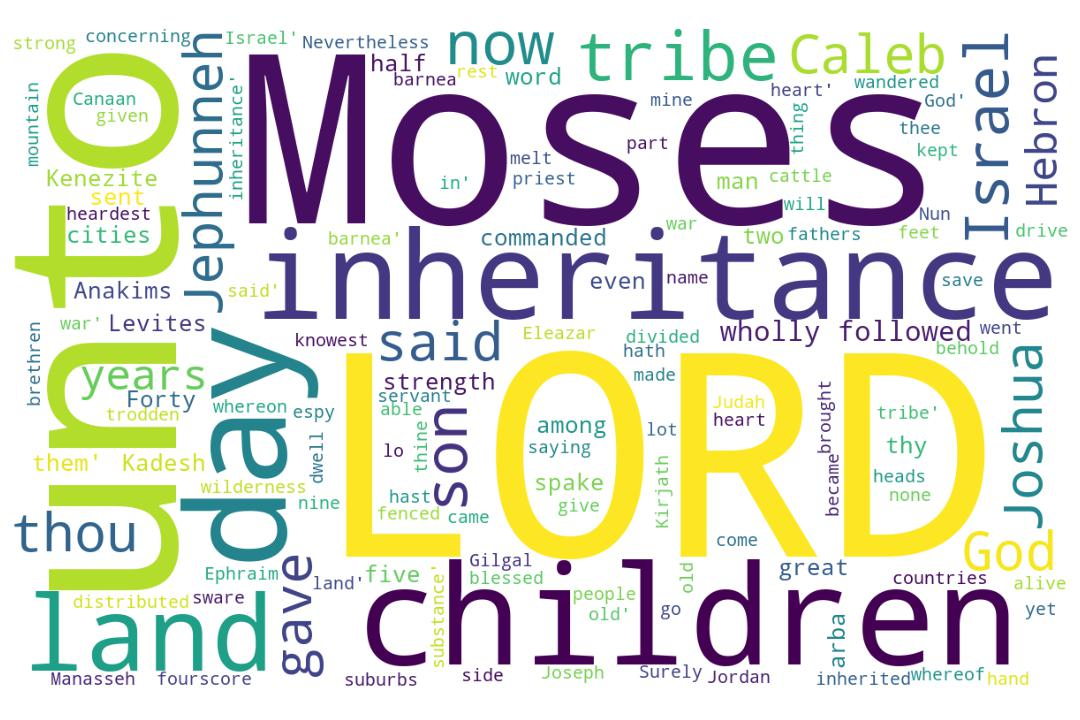
\includegraphics[width=\linewidth]{06OT-Joshua/Joshua14-WordCloud.jpg}
  \caption{Joshua 14 Word Cloud}
  \label{fig:Joshua 14 Word Cloud}
\end{figure}

\marginpar{\scriptsize \centering \fcolorbox{bone}{lime}{\textbf{CALEB'S VEIW}}\\ (Joshua 14) \begin{compactenum}[I.][8]
	\item \textbf{Countries Inherited}  \index[scripture]{Joshua!Jsh 14:01} (Jsh 14:1) 
	\item \textbf{Commands Heeded}  \index[scripture]{Joshua!Jsh 14:05} (Jsh 14:5) 
	\item \textbf{Caleb's Heart}  \index[scripture]{Joshua!Jsh 14:07} (Jsh 14:7) 
	\item A \textbf{Conspicuous Heritage}  \index[scripture]{Joshua!Jsh 14:09} (Jsh 14:9) 
	\item \textbf{Condemned Houses}  \index[scripture]{Joshua!Jsh 14:10} (Jsh 14:10) 
	\item \textbf{Courageous and Healthy}  \index[scripture]{Joshua!Jsh 14:11} (Jsh 14:11) 
\end{compactenum}}




\footnote{\textcolor[rgb]{0.00,0.25,0.00}{\hyperlink{TOC}{Return to end of Table of Contents.}}}\footnote{\href{https://audiobible.com/bible/joshua_14.html}{\textcolor[cmyk]{0.99998,1,0,0}{Joshua 14 Audio}}}\textcolor[cmyk]{0.99998,1,0,0}{And these \emph{are} \emph{the} \fcolorbox{bone}{lime}{\emph{countries}} which the children of Israel inherited in the land of Canaan, which Eleazar the priest, and Joshua the son of Nun, and the heads of the fathers of the tribes of the children of Israel, distributed for inheritance to them.}
[2] \textcolor[cmyk]{0.99998,1,0,0}{By lot \emph{was} their inheritance, as the LORD commanded by the hand of Moses, for the nine tribes, and \emph{for} the half tribe.}
[3] \textcolor[cmyk]{0.99998,1,0,0}{For Moses had given the inheritance of two tribes and an half tribe on the other side Jordan: but unto the Levites he gave none inheritance among them.}
[4] \textcolor[cmyk]{0.99998,1,0,0}{For the children of Joseph were two tribes, Manasseh and Ephraim: therefore they gave no part unto the Levites in the land, save cities to dwell \emph{in}, with their suburbs for their cattle and for their substance.}
[5] \textcolor[cmyk]{0.99998,1,0,0}{As the LORD \fcolorbox{bone}{lime}{commanded} Moses, so the children of Israel did, and they divided the land.}\\
\\
\P \textcolor[cmyk]{0.99998,1,0,0}{Then the children of Judah came unto Joshua in Gilgal: and Caleb the son of Jephunneh the Kenezite said unto him, Thou knowest the thing that the LORD said unto Moses the man of God concerning me and thee in \fcolorbox{bone}{MYGOLD}{Kadesh-barnea}.}
[7] \textcolor[cmyk]{0.99998,1,0,0}{Forty years old \emph{was} I when Moses the servant of the LORD sent me from \fcolorbox{bone}{MYGOLD}{Kadesh-barnea} to espy out the land; and I brought him word again as \emph{it} \emph{was} in \fcolorbox{bone}{lime}{mine heart}.}
[8] \textcolor[cmyk]{0.99998,1,0,0}{Nevertheless my brethren that went up with me made the heart of the people melt: but I wholly followed the LORD my God.}
[9] \textcolor[cmyk]{0.99998,1,0,0}{And Moses sware on that day, saying, Surely the land whereon thy feet have trodden shall be thine \fcolorbox{bone}{lime}{inheritance}, and thy children's for ever, because thou hast wholly followed the LORD my God.}
[10] \textcolor[cmyk]{0.99998,1,0,0}{And now, behold, the LORD hath kept me alive, as he said, these \fcolorbox{bone}{lime}{forty and five years}, even since the LORD spake this word unto Moses, while \emph{the} \emph{children} \emph{of} Israel wandered in the wilderness: and now, lo, I \emph{am} this day fourscore and five years old.}
[11] \textcolor[cmyk]{0.99998,1,0,0}{As yet I \emph{am} \emph{as} strong this day as \emph{I} \emph{was} in the day that Moses sent me: as my strength \emph{was} then, even so \emph{is} my \fcolorbox{bone}{lime}{strength} now, for war, both to go out, and to come in.}
[12] \textcolor[cmyk]{0.99998,1,0,0}{Now therefore give me this mountain, whereof the LORD spake in that day; for thou heardest in that day how the Anakims \emph{were} there, and \emph{that} the cities \emph{were} great \emph{and} fenced: if so be the LORD \emph{will} \emph{be} with me, then I shall be able to drive them out, as the LORD said.}
[13] \textcolor[cmyk]{0.99998,1,0,0}{And Joshua blessed him, and gave unto Caleb the son of Jephunneh Hebron for an inheritance.}
[14] \textcolor[cmyk]{0.99998,1,0,0}{Hebron therefore became the inheritance of Caleb the son of Jephunneh the Kenezite unto this day, because that he wholly followed the LORD God of Israel.}
[15] \textcolor[cmyk]{0.99998,1,0,0}{And the name of Hebron before \emph{was} Kirjath-arba; \emph{which} \emph{Arba} \emph{was} a great man among the Anakims. And the land had rest from war.}
\index[NWIV]{45!Joshua!Jos 14:1}\index[AWIP]{And!Joshua!Jos 14:1}\index[AWIP]{these!Joshua!Jos 14:1}\index[AWIP]{\emph{are}!Joshua!Jos 14:1}\index[AWIP]{\emph{the}!Joshua!Jos 14:1}\index[AWIP]{\emph{countries}!Joshua!Jos 14:1}\index[AWIP]{which!Joshua!Jos 14:1}\index[AWIP]{which!Joshua!Jos 14:1 (2)}\index[AWIP]{the!Joshua!Jos 14:1}\index[AWIP]{the!Joshua!Jos 14:1 (2)}\index[AWIP]{the!Joshua!Jos 14:1 (3)}\index[AWIP]{the!Joshua!Jos 14:1 (4)}\index[AWIP]{the!Joshua!Jos 14:1 (5)}\index[AWIP]{the!Joshua!Jos 14:1 (6)}\index[AWIP]{the!Joshua!Jos 14:1 (7)}\index[AWIP]{the!Joshua!Jos 14:1 (8)}\index[AWIP]{children!Joshua!Jos 14:1}\index[AWIP]{children!Joshua!Jos 14:1 (2)}\index[AWIP]{of!Joshua!Jos 14:1}\index[AWIP]{of!Joshua!Jos 14:1 (2)}\index[AWIP]{of!Joshua!Jos 14:1 (3)}\index[AWIP]{of!Joshua!Jos 14:1 (4)}\index[AWIP]{of!Joshua!Jos 14:1 (5)}\index[AWIP]{of!Joshua!Jos 14:1 (6)}\index[AWIP]{of!Joshua!Jos 14:1 (7)}\index[AWIP]{Israel!Joshua!Jos 14:1}\index[AWIP]{Israel!Joshua!Jos 14:1 (2)}\index[AWIP]{inherited!Joshua!Jos 14:1}\index[AWIP]{in!Joshua!Jos 14:1}\index[AWIP]{land!Joshua!Jos 14:1}\index[AWIP]{Canaan!Joshua!Jos 14:1}\index[AWIP]{Eleazar!Joshua!Jos 14:1}\index[AWIP]{priest!Joshua!Jos 14:1}\index[AWIP]{and!Joshua!Jos 14:1}\index[AWIP]{and!Joshua!Jos 14:1 (2)}\index[AWIP]{Joshua!Joshua!Jos 14:1}\index[AWIP]{son!Joshua!Jos 14:1}\index[AWIP]{Nun!Joshua!Jos 14:1}\index[AWIP]{heads!Joshua!Jos 14:1}\index[AWIP]{fathers!Joshua!Jos 14:1}\index[AWIP]{tribes!Joshua!Jos 14:1}\index[AWIP]{distributed!Joshua!Jos 14:1}\index[AWIP]{for!Joshua!Jos 14:1}\index[AWIP]{inheritance!Joshua!Jos 14:1}\index[AWIP]{to!Joshua!Jos 14:1}\index[AWIP]{them!Joshua!Jos 14:1}\index[AWIP]{\emph{are}!Joshua!Jos 14:1}\index[AWIP]{\emph{the}!Joshua!Jos 14:1}\index[AWIP]{\emph{countries}!Joshua!Jos 14:1}

\index[NWIV]{23!Joshua!Jos 14:2}\index[AWIP]{By!Joshua!Jos 14:2}\index[AWIP]{lot!Joshua!Jos 14:2}\index[AWIP]{\emph{was}!Joshua!Jos 14:2}\index[AWIP]{their!Joshua!Jos 14:2}\index[AWIP]{inheritance!Joshua!Jos 14:2}\index[AWIP]{as!Joshua!Jos 14:2}\index[AWIP]{the!Joshua!Jos 14:2}\index[AWIP]{the!Joshua!Jos 14:2 (2)}\index[AWIP]{the!Joshua!Jos 14:2 (3)}\index[AWIP]{the!Joshua!Jos 14:2 (4)}\index[AWIP]{LORD!Joshua!Jos 14:2}\index[AWIP]{commanded!Joshua!Jos 14:2}\index[AWIP]{by!Joshua!Jos 14:2}\index[AWIP]{hand!Joshua!Jos 14:2}\index[AWIP]{of!Joshua!Jos 14:2}\index[AWIP]{Moses!Joshua!Jos 14:2}\index[AWIP]{for!Joshua!Jos 14:2}\index[AWIP]{nine!Joshua!Jos 14:2}\index[AWIP]{tribes!Joshua!Jos 14:2}\index[AWIP]{and!Joshua!Jos 14:2}\index[AWIP]{\emph{for}!Joshua!Jos 14:2}\index[AWIP]{half!Joshua!Jos 14:2}\index[AWIP]{tribe!Joshua!Jos 14:2}\index[AWIP]{\emph{was}!Joshua!Jos 14:2}\index[AWIP]{\emph{for}!Joshua!Jos 14:2}

\index[NWIV]{28!Joshua!Jos 14:3}\index[AWIP]{For!Joshua!Jos 14:3}\index[AWIP]{Moses!Joshua!Jos 14:3}\index[AWIP]{had!Joshua!Jos 14:3}\index[AWIP]{given!Joshua!Jos 14:3}\index[AWIP]{the!Joshua!Jos 14:3}\index[AWIP]{the!Joshua!Jos 14:3 (2)}\index[AWIP]{the!Joshua!Jos 14:3 (3)}\index[AWIP]{inheritance!Joshua!Jos 14:3}\index[AWIP]{inheritance!Joshua!Jos 14:3 (2)}\index[AWIP]{of!Joshua!Jos 14:3}\index[AWIP]{two!Joshua!Jos 14:3}\index[AWIP]{tribes!Joshua!Jos 14:3}\index[AWIP]{and!Joshua!Jos 14:3}\index[AWIP]{an!Joshua!Jos 14:3}\index[AWIP]{half!Joshua!Jos 14:3}\index[AWIP]{tribe!Joshua!Jos 14:3}\index[AWIP]{on!Joshua!Jos 14:3}\index[AWIP]{other!Joshua!Jos 14:3}\index[AWIP]{side!Joshua!Jos 14:3}\index[AWIP]{Jordan!Joshua!Jos 14:3}\index[AWIP]{but!Joshua!Jos 14:3}\index[AWIP]{unto!Joshua!Jos 14:3}\index[AWIP]{Levites!Joshua!Jos 14:3}\index[AWIP]{he!Joshua!Jos 14:3}\index[AWIP]{gave!Joshua!Jos 14:3}\index[AWIP]{none!Joshua!Jos 14:3}\index[AWIP]{among!Joshua!Jos 14:3}\index[AWIP]{them!Joshua!Jos 14:3}

\index[NWIV]{37!Joshua!Jos 14:4}\index[AWIP]{For!Joshua!Jos 14:4}\index[AWIP]{the!Joshua!Jos 14:4}\index[AWIP]{the!Joshua!Jos 14:4 (2)}\index[AWIP]{the!Joshua!Jos 14:4 (3)}\index[AWIP]{children!Joshua!Jos 14:4}\index[AWIP]{of!Joshua!Jos 14:4}\index[AWIP]{Joseph!Joshua!Jos 14:4}\index[AWIP]{were!Joshua!Jos 14:4}\index[AWIP]{two!Joshua!Jos 14:4}\index[AWIP]{tribes!Joshua!Jos 14:4}\index[AWIP]{Manasseh!Joshua!Jos 14:4}\index[AWIP]{and!Joshua!Jos 14:4}\index[AWIP]{and!Joshua!Jos 14:4 (2)}\index[AWIP]{Ephraim!Joshua!Jos 14:4}\index[AWIP]{therefore!Joshua!Jos 14:4}\index[AWIP]{they!Joshua!Jos 14:4}\index[AWIP]{gave!Joshua!Jos 14:4}\index[AWIP]{no!Joshua!Jos 14:4}\index[AWIP]{part!Joshua!Jos 14:4}\index[AWIP]{unto!Joshua!Jos 14:4}\index[AWIP]{Levites!Joshua!Jos 14:4}\index[AWIP]{in!Joshua!Jos 14:4}\index[AWIP]{land!Joshua!Jos 14:4}\index[AWIP]{save!Joshua!Jos 14:4}\index[AWIP]{cities!Joshua!Jos 14:4}\index[AWIP]{to!Joshua!Jos 14:4}\index[AWIP]{dwell!Joshua!Jos 14:4}\index[AWIP]{\emph{in}!Joshua!Jos 14:4}\index[AWIP]{with!Joshua!Jos 14:4}\index[AWIP]{their!Joshua!Jos 14:4}\index[AWIP]{their!Joshua!Jos 14:4 (2)}\index[AWIP]{their!Joshua!Jos 14:4 (3)}\index[AWIP]{suburbs!Joshua!Jos 14:4}\index[AWIP]{for!Joshua!Jos 14:4}\index[AWIP]{for!Joshua!Jos 14:4 (2)}\index[AWIP]{cattle!Joshua!Jos 14:4}\index[AWIP]{substance!Joshua!Jos 14:4}\index[AWIP]{\emph{in}!Joshua!Jos 14:4}

\index[NWIV]{16!Joshua!Jos 14:5}\index[AWIP]{As!Joshua!Jos 14:5}\index[AWIP]{the!Joshua!Jos 14:5}\index[AWIP]{the!Joshua!Jos 14:5 (2)}\index[AWIP]{the!Joshua!Jos 14:5 (3)}\index[AWIP]{LORD!Joshua!Jos 14:5}\index[AWIP]{commanded!Joshua!Jos 14:5}\index[AWIP]{Moses!Joshua!Jos 14:5}\index[AWIP]{so!Joshua!Jos 14:5}\index[AWIP]{children!Joshua!Jos 14:5}\index[AWIP]{of!Joshua!Jos 14:5}\index[AWIP]{Israel!Joshua!Jos 14:5}\index[AWIP]{did!Joshua!Jos 14:5}\index[AWIP]{and!Joshua!Jos 14:5}\index[AWIP]{they!Joshua!Jos 14:5}\index[AWIP]{divided!Joshua!Jos 14:5}\index[AWIP]{land!Joshua!Jos 14:5}

\index[NWIV]{41!Joshua!Jos 14:6}\index[AWIP]{Then!Joshua!Jos 14:6}\index[AWIP]{the!Joshua!Jos 14:6}\index[AWIP]{the!Joshua!Jos 14:6 (2)}\index[AWIP]{the!Joshua!Jos 14:6 (3)}\index[AWIP]{the!Joshua!Jos 14:6 (4)}\index[AWIP]{the!Joshua!Jos 14:6 (5)}\index[AWIP]{the!Joshua!Jos 14:6 (6)}\index[AWIP]{children!Joshua!Jos 14:6}\index[AWIP]{of!Joshua!Jos 14:6}\index[AWIP]{of!Joshua!Jos 14:6 (2)}\index[AWIP]{of!Joshua!Jos 14:6 (3)}\index[AWIP]{Judah!Joshua!Jos 14:6}\index[AWIP]{came!Joshua!Jos 14:6}\index[AWIP]{unto!Joshua!Jos 14:6}\index[AWIP]{unto!Joshua!Jos 14:6 (2)}\index[AWIP]{unto!Joshua!Jos 14:6 (3)}\index[AWIP]{Joshua!Joshua!Jos 14:6}\index[AWIP]{in!Joshua!Jos 14:6}\index[AWIP]{in!Joshua!Jos 14:6 (2)}\index[AWIP]{Gilgal!Joshua!Jos 14:6}\index[AWIP]{and!Joshua!Jos 14:6}\index[AWIP]{and!Joshua!Jos 14:6 (2)}\index[AWIP]{Caleb!Joshua!Jos 14:6}\index[AWIP]{son!Joshua!Jos 14:6}\index[AWIP]{Jephunneh!Joshua!Jos 14:6}\index[AWIP]{Kenezite!Joshua!Jos 14:6}\index[AWIP]{said!Joshua!Jos 14:6}\index[AWIP]{said!Joshua!Jos 14:6 (2)}\index[AWIP]{him!Joshua!Jos 14:6}\index[AWIP]{Thou!Joshua!Jos 14:6}\index[AWIP]{knowest!Joshua!Jos 14:6}\index[AWIP]{thing!Joshua!Jos 14:6}\index[AWIP]{that!Joshua!Jos 14:6}\index[AWIP]{LORD!Joshua!Jos 14:6}\index[AWIP]{Moses!Joshua!Jos 14:6}\index[AWIP]{man!Joshua!Jos 14:6}\index[AWIP]{God!Joshua!Jos 14:6}\index[AWIP]{concerning!Joshua!Jos 14:6}\index[AWIP]{me!Joshua!Jos 14:6}\index[AWIP]{thee!Joshua!Jos 14:6}\index[AWIP]{Kadesh-barnea!Joshua!Jos 14:6}

\index[NWIV]{33!Joshua!Jos 14:7}\index[AWIP]{Forty!Joshua!Jos 14:7}\index[AWIP]{years!Joshua!Jos 14:7}\index[AWIP]{old!Joshua!Jos 14:7}\index[AWIP]{\emph{was}!Joshua!Jos 14:7}\index[AWIP]{\emph{was}!Joshua!Jos 14:7 (2)}\index[AWIP]{I!Joshua!Jos 14:7}\index[AWIP]{I!Joshua!Jos 14:7 (2)}\index[AWIP]{when!Joshua!Jos 14:7}\index[AWIP]{Moses!Joshua!Jos 14:7}\index[AWIP]{the!Joshua!Jos 14:7}\index[AWIP]{the!Joshua!Jos 14:7 (2)}\index[AWIP]{the!Joshua!Jos 14:7 (3)}\index[AWIP]{servant!Joshua!Jos 14:7}\index[AWIP]{of!Joshua!Jos 14:7}\index[AWIP]{LORD!Joshua!Jos 14:7}\index[AWIP]{sent!Joshua!Jos 14:7}\index[AWIP]{me!Joshua!Jos 14:7}\index[AWIP]{from!Joshua!Jos 14:7}\index[AWIP]{Kadesh-barnea!Joshua!Jos 14:7}\index[AWIP]{to!Joshua!Jos 14:7}\index[AWIP]{espy!Joshua!Jos 14:7}\index[AWIP]{out!Joshua!Jos 14:7}\index[AWIP]{land!Joshua!Jos 14:7}\index[AWIP]{and!Joshua!Jos 14:7}\index[AWIP]{brought!Joshua!Jos 14:7}\index[AWIP]{him!Joshua!Jos 14:7}\index[AWIP]{word!Joshua!Jos 14:7}\index[AWIP]{again!Joshua!Jos 14:7}\index[AWIP]{as!Joshua!Jos 14:7}\index[AWIP]{\emph{it}!Joshua!Jos 14:7}\index[AWIP]{in!Joshua!Jos 14:7}\index[AWIP]{mine!Joshua!Jos 14:7}\index[AWIP]{heart!Joshua!Jos 14:7}\index[AWIP]{\emph{was}!Joshua!Jos 14:7}\index[AWIP]{\emph{was}!Joshua!Jos 14:7 (2)}\index[AWIP]{\emph{it}!Joshua!Jos 14:7}

\index[NWIV]{23!Joshua!Jos 14:8}\index[AWIP]{Nevertheless!Joshua!Jos 14:8}\index[AWIP]{my!Joshua!Jos 14:8}\index[AWIP]{my!Joshua!Jos 14:8 (2)}\index[AWIP]{brethren!Joshua!Jos 14:8}\index[AWIP]{that!Joshua!Jos 14:8}\index[AWIP]{went!Joshua!Jos 14:8}\index[AWIP]{up!Joshua!Jos 14:8}\index[AWIP]{with!Joshua!Jos 14:8}\index[AWIP]{me!Joshua!Jos 14:8}\index[AWIP]{made!Joshua!Jos 14:8}\index[AWIP]{the!Joshua!Jos 14:8}\index[AWIP]{the!Joshua!Jos 14:8 (2)}\index[AWIP]{the!Joshua!Jos 14:8 (3)}\index[AWIP]{heart!Joshua!Jos 14:8}\index[AWIP]{of!Joshua!Jos 14:8}\index[AWIP]{people!Joshua!Jos 14:8}\index[AWIP]{melt!Joshua!Jos 14:8}\index[AWIP]{but!Joshua!Jos 14:8}\index[AWIP]{I!Joshua!Jos 14:8}\index[AWIP]{wholly!Joshua!Jos 14:8}\index[AWIP]{followed!Joshua!Jos 14:8}\index[AWIP]{LORD!Joshua!Jos 14:8}\index[AWIP]{God!Joshua!Jos 14:8}

\index[NWIV]{33!Joshua!Jos 14:9}\index[AWIP]{And!Joshua!Jos 14:9}\index[AWIP]{Moses!Joshua!Jos 14:9}\index[AWIP]{sware!Joshua!Jos 14:9}\index[AWIP]{on!Joshua!Jos 14:9}\index[AWIP]{that!Joshua!Jos 14:9}\index[AWIP]{day!Joshua!Jos 14:9}\index[AWIP]{saying!Joshua!Jos 14:9}\index[AWIP]{Surely!Joshua!Jos 14:9}\index[AWIP]{the!Joshua!Jos 14:9}\index[AWIP]{the!Joshua!Jos 14:9 (2)}\index[AWIP]{land!Joshua!Jos 14:9}\index[AWIP]{whereon!Joshua!Jos 14:9}\index[AWIP]{thy!Joshua!Jos 14:9}\index[AWIP]{thy!Joshua!Jos 14:9 (2)}\index[AWIP]{feet!Joshua!Jos 14:9}\index[AWIP]{have!Joshua!Jos 14:9}\index[AWIP]{trodden!Joshua!Jos 14:9}\index[AWIP]{shall!Joshua!Jos 14:9}\index[AWIP]{be!Joshua!Jos 14:9}\index[AWIP]{thine!Joshua!Jos 14:9}\index[AWIP]{inheritance!Joshua!Jos 14:9}\index[AWIP]{and!Joshua!Jos 14:9}\index[AWIP]{children's!Joshua!Jos 14:9}\index[AWIP]{for!Joshua!Jos 14:9}\index[AWIP]{ever!Joshua!Jos 14:9}\index[AWIP]{because!Joshua!Jos 14:9}\index[AWIP]{thou!Joshua!Jos 14:9}\index[AWIP]{hast!Joshua!Jos 14:9}\index[AWIP]{wholly!Joshua!Jos 14:9}\index[AWIP]{followed!Joshua!Jos 14:9}\index[AWIP]{LORD!Joshua!Jos 14:9}\index[AWIP]{my!Joshua!Jos 14:9}\index[AWIP]{God!Joshua!Jos 14:9}

\index[NWIV]{47!Joshua!Jos 14:10}\index[AWIP]{And!Joshua!Jos 14:10}\index[AWIP]{now!Joshua!Jos 14:10}\index[AWIP]{now!Joshua!Jos 14:10 (2)}\index[AWIP]{behold!Joshua!Jos 14:10}\index[AWIP]{the!Joshua!Jos 14:10}\index[AWIP]{the!Joshua!Jos 14:10 (2)}\index[AWIP]{the!Joshua!Jos 14:10 (3)}\index[AWIP]{LORD!Joshua!Jos 14:10}\index[AWIP]{LORD!Joshua!Jos 14:10 (2)}\index[AWIP]{hath!Joshua!Jos 14:10}\index[AWIP]{kept!Joshua!Jos 14:10}\index[AWIP]{me!Joshua!Jos 14:10}\index[AWIP]{alive!Joshua!Jos 14:10}\index[AWIP]{as!Joshua!Jos 14:10}\index[AWIP]{he!Joshua!Jos 14:10}\index[AWIP]{said!Joshua!Jos 14:10}\index[AWIP]{these!Joshua!Jos 14:10}\index[AWIP]{forty!Joshua!Jos 14:10}\index[AWIP]{and!Joshua!Jos 14:10}\index[AWIP]{and!Joshua!Jos 14:10 (2)}\index[AWIP]{and!Joshua!Jos 14:10 (3)}\index[AWIP]{five!Joshua!Jos 14:10}\index[AWIP]{five!Joshua!Jos 14:10 (2)}\index[AWIP]{years!Joshua!Jos 14:10}\index[AWIP]{years!Joshua!Jos 14:10 (2)}\index[AWIP]{even!Joshua!Jos 14:10}\index[AWIP]{since!Joshua!Jos 14:10}\index[AWIP]{spake!Joshua!Jos 14:10}\index[AWIP]{this!Joshua!Jos 14:10}\index[AWIP]{this!Joshua!Jos 14:10 (2)}\index[AWIP]{word!Joshua!Jos 14:10}\index[AWIP]{unto!Joshua!Jos 14:10}\index[AWIP]{Moses!Joshua!Jos 14:10}\index[AWIP]{while!Joshua!Jos 14:10}\index[AWIP]{\emph{the}!Joshua!Jos 14:10}\index[AWIP]{\emph{children}!Joshua!Jos 14:10}\index[AWIP]{\emph{of}!Joshua!Jos 14:10}\index[AWIP]{Israel!Joshua!Jos 14:10}\index[AWIP]{wandered!Joshua!Jos 14:10}\index[AWIP]{in!Joshua!Jos 14:10}\index[AWIP]{wilderness!Joshua!Jos 14:10}\index[AWIP]{lo!Joshua!Jos 14:10}\index[AWIP]{I!Joshua!Jos 14:10}\index[AWIP]{\emph{am}!Joshua!Jos 14:10}\index[AWIP]{day!Joshua!Jos 14:10}\index[AWIP]{fourscore!Joshua!Jos 14:10}\index[AWIP]{old!Joshua!Jos 14:10}\index[AWIP]{\emph{the}!Joshua!Jos 14:10}\index[AWIP]{\emph{children}!Joshua!Jos 14:10}\index[AWIP]{\emph{of}!Joshua!Jos 14:10}\index[AWIP]{\emph{am}!Joshua!Jos 14:10}

\index[NWIV]{39!Joshua!Jos 14:11}\index[AWIP]{As!Joshua!Jos 14:11}\index[AWIP]{yet!Joshua!Jos 14:11}\index[AWIP]{I!Joshua!Jos 14:11}\index[AWIP]{\emph{am}!Joshua!Jos 14:11}\index[AWIP]{\emph{as}!Joshua!Jos 14:11}\index[AWIP]{strong!Joshua!Jos 14:11}\index[AWIP]{this!Joshua!Jos 14:11}\index[AWIP]{day!Joshua!Jos 14:11}\index[AWIP]{day!Joshua!Jos 14:11 (2)}\index[AWIP]{as!Joshua!Jos 14:11}\index[AWIP]{as!Joshua!Jos 14:11 (2)}\index[AWIP]{\emph{I}!Joshua!Jos 14:11}\index[AWIP]{\emph{was}!Joshua!Jos 14:11}\index[AWIP]{\emph{was}!Joshua!Jos 14:11 (2)}\index[AWIP]{in!Joshua!Jos 14:11}\index[AWIP]{in!Joshua!Jos 14:11 (2)}\index[AWIP]{the!Joshua!Jos 14:11}\index[AWIP]{that!Joshua!Jos 14:11}\index[AWIP]{Moses!Joshua!Jos 14:11}\index[AWIP]{sent!Joshua!Jos 14:11}\index[AWIP]{me!Joshua!Jos 14:11}\index[AWIP]{my!Joshua!Jos 14:11}\index[AWIP]{my!Joshua!Jos 14:11 (2)}\index[AWIP]{strength!Joshua!Jos 14:11}\index[AWIP]{strength!Joshua!Jos 14:11 (2)}\index[AWIP]{then!Joshua!Jos 14:11}\index[AWIP]{even!Joshua!Jos 14:11}\index[AWIP]{so!Joshua!Jos 14:11}\index[AWIP]{\emph{is}!Joshua!Jos 14:11}\index[AWIP]{now!Joshua!Jos 14:11}\index[AWIP]{for!Joshua!Jos 14:11}\index[AWIP]{war!Joshua!Jos 14:11}\index[AWIP]{both!Joshua!Jos 14:11}\index[AWIP]{to!Joshua!Jos 14:11}\index[AWIP]{to!Joshua!Jos 14:11 (2)}\index[AWIP]{go!Joshua!Jos 14:11}\index[AWIP]{out!Joshua!Jos 14:11}\index[AWIP]{and!Joshua!Jos 14:11}\index[AWIP]{come!Joshua!Jos 14:11}\index[AWIP]{\emph{am}!Joshua!Jos 14:11}\index[AWIP]{\emph{as}!Joshua!Jos 14:11}\index[AWIP]{\emph{I}!Joshua!Jos 14:11}\index[AWIP]{\emph{was}!Joshua!Jos 14:11}\index[AWIP]{\emph{was}!Joshua!Jos 14:11 (2)}\index[AWIP]{\emph{is}!Joshua!Jos 14:11}

\index[NWIV]{54!Joshua!Jos 14:12}\index[AWIP]{Now!Joshua!Jos 14:12}\index[AWIP]{therefore!Joshua!Jos 14:12}\index[AWIP]{give!Joshua!Jos 14:12}\index[AWIP]{me!Joshua!Jos 14:12}\index[AWIP]{me!Joshua!Jos 14:12 (2)}\index[AWIP]{this!Joshua!Jos 14:12}\index[AWIP]{mountain!Joshua!Jos 14:12}\index[AWIP]{whereof!Joshua!Jos 14:12}\index[AWIP]{the!Joshua!Jos 14:12}\index[AWIP]{the!Joshua!Jos 14:12 (2)}\index[AWIP]{the!Joshua!Jos 14:12 (3)}\index[AWIP]{the!Joshua!Jos 14:12 (4)}\index[AWIP]{the!Joshua!Jos 14:12 (5)}\index[AWIP]{LORD!Joshua!Jos 14:12}\index[AWIP]{LORD!Joshua!Jos 14:12 (2)}\index[AWIP]{LORD!Joshua!Jos 14:12 (3)}\index[AWIP]{spake!Joshua!Jos 14:12}\index[AWIP]{in!Joshua!Jos 14:12}\index[AWIP]{in!Joshua!Jos 14:12 (2)}\index[AWIP]{that!Joshua!Jos 14:12}\index[AWIP]{that!Joshua!Jos 14:12 (2)}\index[AWIP]{day!Joshua!Jos 14:12}\index[AWIP]{day!Joshua!Jos 14:12 (2)}\index[AWIP]{for!Joshua!Jos 14:12}\index[AWIP]{thou!Joshua!Jos 14:12}\index[AWIP]{heardest!Joshua!Jos 14:12}\index[AWIP]{how!Joshua!Jos 14:12}\index[AWIP]{Anakims!Joshua!Jos 14:12}\index[AWIP]{\emph{were}!Joshua!Jos 14:12}\index[AWIP]{\emph{were}!Joshua!Jos 14:12 (2)}\index[AWIP]{there!Joshua!Jos 14:12}\index[AWIP]{and!Joshua!Jos 14:12}\index[AWIP]{\emph{that}!Joshua!Jos 14:12}\index[AWIP]{cities!Joshua!Jos 14:12}\index[AWIP]{great!Joshua!Jos 14:12}\index[AWIP]{\emph{and}!Joshua!Jos 14:12}\index[AWIP]{fenced!Joshua!Jos 14:12}\index[AWIP]{if!Joshua!Jos 14:12}\index[AWIP]{so!Joshua!Jos 14:12}\index[AWIP]{be!Joshua!Jos 14:12}\index[AWIP]{be!Joshua!Jos 14:12 (2)}\index[AWIP]{\emph{will}!Joshua!Jos 14:12}\index[AWIP]{\emph{be}!Joshua!Jos 14:12}\index[AWIP]{with!Joshua!Jos 14:12}\index[AWIP]{then!Joshua!Jos 14:12}\index[AWIP]{I!Joshua!Jos 14:12}\index[AWIP]{shall!Joshua!Jos 14:12}\index[AWIP]{able!Joshua!Jos 14:12}\index[AWIP]{to!Joshua!Jos 14:12}\index[AWIP]{drive!Joshua!Jos 14:12}\index[AWIP]{them!Joshua!Jos 14:12}\index[AWIP]{out!Joshua!Jos 14:12}\index[AWIP]{as!Joshua!Jos 14:12}\index[AWIP]{said!Joshua!Jos 14:12}\index[AWIP]{\emph{were}!Joshua!Jos 14:12}\index[AWIP]{\emph{were}!Joshua!Jos 14:12 (2)}\index[AWIP]{\emph{that}!Joshua!Jos 14:12}\index[AWIP]{\emph{and}!Joshua!Jos 14:12}\index[AWIP]{\emph{will}!Joshua!Jos 14:12}\index[AWIP]{\emph{be}!Joshua!Jos 14:12}

\index[NWIV]{16!Joshua!Jos 14:13}\index[AWIP]{And!Joshua!Jos 14:13}\index[AWIP]{Joshua!Joshua!Jos 14:13}\index[AWIP]{blessed!Joshua!Jos 14:13}\index[AWIP]{him!Joshua!Jos 14:13}\index[AWIP]{and!Joshua!Jos 14:13}\index[AWIP]{gave!Joshua!Jos 14:13}\index[AWIP]{unto!Joshua!Jos 14:13}\index[AWIP]{Caleb!Joshua!Jos 14:13}\index[AWIP]{the!Joshua!Jos 14:13}\index[AWIP]{son!Joshua!Jos 14:13}\index[AWIP]{of!Joshua!Jos 14:13}\index[AWIP]{Jephunneh!Joshua!Jos 14:13}\index[AWIP]{Hebron!Joshua!Jos 14:13}\index[AWIP]{for!Joshua!Jos 14:13}\index[AWIP]{an!Joshua!Jos 14:13}\index[AWIP]{inheritance!Joshua!Jos 14:13}

\index[NWIV]{26!Joshua!Jos 14:14}\index[AWIP]{Hebron!Joshua!Jos 14:14}\index[AWIP]{therefore!Joshua!Jos 14:14}\index[AWIP]{became!Joshua!Jos 14:14}\index[AWIP]{the!Joshua!Jos 14:14}\index[AWIP]{the!Joshua!Jos 14:14 (2)}\index[AWIP]{the!Joshua!Jos 14:14 (3)}\index[AWIP]{the!Joshua!Jos 14:14 (4)}\index[AWIP]{inheritance!Joshua!Jos 14:14}\index[AWIP]{of!Joshua!Jos 14:14}\index[AWIP]{of!Joshua!Jos 14:14 (2)}\index[AWIP]{of!Joshua!Jos 14:14 (3)}\index[AWIP]{Caleb!Joshua!Jos 14:14}\index[AWIP]{son!Joshua!Jos 14:14}\index[AWIP]{Jephunneh!Joshua!Jos 14:14}\index[AWIP]{Kenezite!Joshua!Jos 14:14}\index[AWIP]{unto!Joshua!Jos 14:14}\index[AWIP]{this!Joshua!Jos 14:14}\index[AWIP]{day!Joshua!Jos 14:14}\index[AWIP]{because!Joshua!Jos 14:14}\index[AWIP]{that!Joshua!Jos 14:14}\index[AWIP]{he!Joshua!Jos 14:14}\index[AWIP]{wholly!Joshua!Jos 14:14}\index[AWIP]{followed!Joshua!Jos 14:14}\index[AWIP]{LORD!Joshua!Jos 14:14}\index[AWIP]{God!Joshua!Jos 14:14}\index[AWIP]{Israel!Joshua!Jos 14:14}

\index[NWIV]{24!Joshua!Jos 14:15}\index[AWIP]{And!Joshua!Jos 14:15}\index[AWIP]{And!Joshua!Jos 14:15 (2)}\index[AWIP]{the!Joshua!Jos 14:15}\index[AWIP]{the!Joshua!Jos 14:15 (2)}\index[AWIP]{the!Joshua!Jos 14:15 (3)}\index[AWIP]{name!Joshua!Jos 14:15}\index[AWIP]{of!Joshua!Jos 14:15}\index[AWIP]{Hebron!Joshua!Jos 14:15}\index[AWIP]{before!Joshua!Jos 14:15}\index[AWIP]{\emph{was}!Joshua!Jos 14:15}\index[AWIP]{\emph{was}!Joshua!Jos 14:15 (2)}\index[AWIP]{Kirjath-arba!Joshua!Jos 14:15}\index[AWIP]{\emph{which}!Joshua!Jos 14:15}\index[AWIP]{\emph{Arba}!Joshua!Jos 14:15}\index[AWIP]{a!Joshua!Jos 14:15}\index[AWIP]{great!Joshua!Jos 14:15}\index[AWIP]{man!Joshua!Jos 14:15}\index[AWIP]{among!Joshua!Jos 14:15}\index[AWIP]{Anakims!Joshua!Jos 14:15}\index[AWIP]{land!Joshua!Jos 14:15}\index[AWIP]{had!Joshua!Jos 14:15}\index[AWIP]{rest!Joshua!Jos 14:15}\index[AWIP]{from!Joshua!Jos 14:15}\index[AWIP]{war!Joshua!Jos 14:15}\index[AWIP]{\emph{was}!Joshua!Jos 14:15}\index[AWIP]{\emph{was}!Joshua!Jos 14:15 (2)}\index[AWIP]{\emph{which}!Joshua!Jos 14:15}\index[AWIP]{\emph{Arba}!Joshua!Jos 14:15}


\section{Joshua 14 Outlines}

\subsection{My Outlines}

\subsubsection{Caleb's View}
\index[speaker]{Keith Anthony!Joshua 14 (Caleb's View}
\index[series]{Joshua (Keith Anthony)!Joshua 14 (Caleb's View)}
\index[date]{2018/03/09!Joshua 14 (Caleb's View) (Keith Anthony)}
\begin{compactenum}[I.]
	\item \textbf{Countries Inherited}  \index[scripture]{Joshua!Jsh 14:01} (Jsh 14:1) 
	\item \textbf{Commands Heeded}  \index[scripture]{Joshua!Jsh 14:05} (Jsh 14:5) 
	\item \textbf{Caleb's Heart}  \index[scripture]{Joshua!Jsh 14:07} (Jsh 14:7) 
	\item A \textbf{Conspicuous Heritage}  \index[scripture]{Joshua!Jsh 14:09} (Jsh 14:9) 
	\item \textbf{Condemned Houses}  \index[scripture]{Joshua!Jsh 14:10} (Jsh 14:10) 
	\item \textbf{Courageous and Healthy}  \index[scripture]{Joshua!Jsh 14:11} (Jsh 14:11) 
\end{compactenum}
\subsection{My Outlines from Others}


\section{Joshua 14 Comments}

\subsection{Numeric Nuggets}
\textbf{13: } The 13-letter name ``Kadesh-barnea'' is found in verses 6 and 7.


\chapter{Joshua 15}

\begin{figure}
  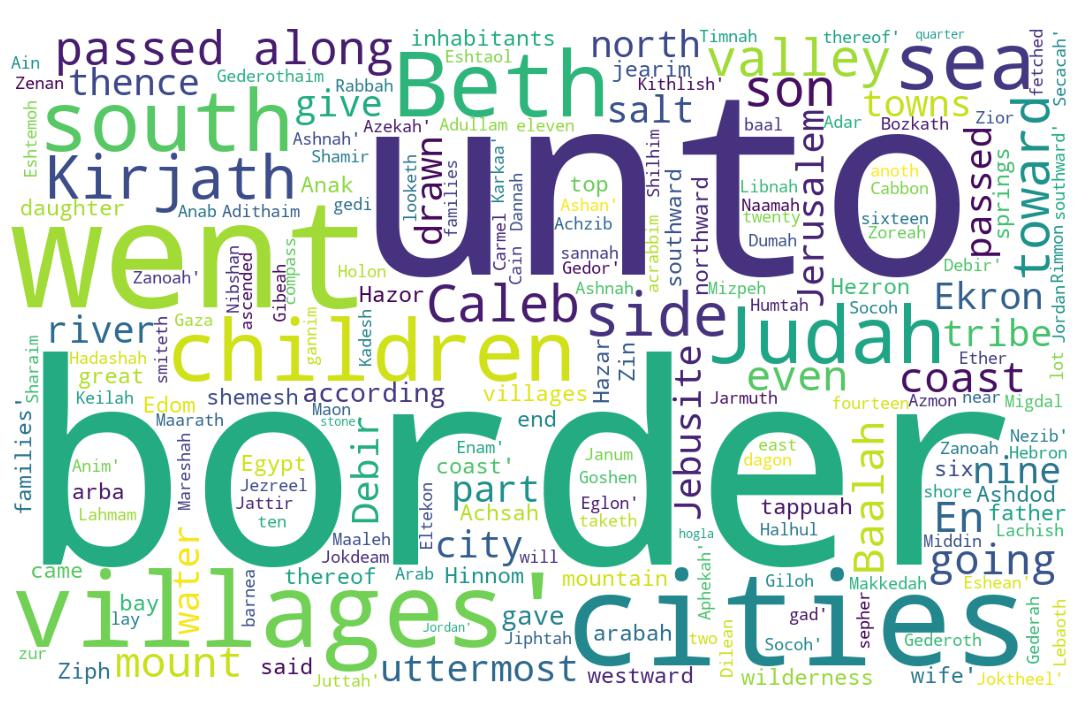
\includegraphics[width=\linewidth]{06OT-Joshua/Joshua15-WordCloud.jpg}
  \caption{Joshua 15 Word Cloud}
  \label{fig:Joshua 15 Word Cloud}
\end{figure}

\marginpar{\scriptsize \centering \fcolorbox{bone}{lime}{\textbf{LAND FOR JUDAH}}\\ (Joshua 15)

\begin{compactenum}[I.][8]

	\item \textbf{Judah's Children}  \index[scripture]{Joshua!Jsh 15:01} (Jsh 15:1) 
	\item The Sea \textbf{Coast}  \index[scripture]{Joshua!Jsh 15:02} (Jsh 15:2) 
	\item Caleb's \textbf{Cutout}  \index[scripture]{Joshua!Jsh 15:13--19} (Jsh 15:13--19) 
	\item \textbf{Cities} Prebuilt \index[scripture]{Joshua!Jsh 15:20--61} (Jsh 15:20--61) 
	\item Incomplete \textbf{Conquest}  \index[scripture]{Joshua!Jsh 15:63} (Jsh 15:63) 
	\item A \textbf{Concern} for Detail %\index[scripture]{Joshua!Jsh 15:13--19} (Jsh 15:13--19) 

\end{compactenum}}





\footnote{\textcolor[rgb]{0.00,0.25,0.00}{\hyperlink{TOC}{Return to end of Table of Contents.}}}\footnote{\href{https://audiobible.com/bible/joshua_15.html}{\textcolor[cmyk]{0.99998,1,0,0}{Joshua 15 Audio}}}\textcolor[cmyk]{0.99998,1,0,0}{\emph{This} then was the lot of the tribe of the children of Judah by their families; \emph{even} to the border of Edom the wilderness of Zin southward \emph{was} the uttermost part of the south coast.}
[2] \textcolor[cmyk]{0.99998,1,0,0}{And their south border was from the shore of the salt sea, from the bay that looketh southward:}
[3] \textcolor[cmyk]{0.99998,1,0,0}{And it \fcolorbox{bone}{bone}{went} out to the south side to Maaleh-acrabbim, and passed along to Zin, and ascended up on the south side unto \fcolorbox{bone}{MYGOLD}{Kadesh-barnea}, and passed along to Hezron, and \fcolorbox{bone}{bone}{went} up to Adar, and fetched a compass to Karkaa:}
[4] \textcolor[cmyk]{0.99998,1,0,0}{\emph{From} \emph{thence} it passed toward Azmon, and \fcolorbox{bone}{bone}{went} out unto the river of Egypt; and the goings out of that coast were at the sea: this shall be your south coast.}
[5] \textcolor[cmyk]{0.99998,1,0,0}{And the east border \emph{was} the salt sea, \emph{even} unto the end of Jordan. And \emph{their} border in the north quarter \emph{was} from the bay of the sea at the uttermost part of Jordan:}
[6] \textcolor[cmyk]{0.99998,1,0,0}{And the border \fcolorbox{bone}{bone}{went} up to Beth-hogla, and passed along by the north of Beth-arabah; and the border \fcolorbox{bone}{bone}{went} up to the stone of Bohan the son of Reuben:}
[7] \textcolor[cmyk]{0.99998,1,0,0}{And the border \fcolorbox{bone}{bone}{went} up toward Debir from the valley of Achor, and so northward, looking toward Gilgal, that \fcolorbox{bone}{bone}{\emph{is}}  before the going up to Adummim, which \fcolorbox{bone}{bone}{\emph{is}}  on the south side of the river: and the border passed toward the waters of En-shemesh, and the goings out thereof were at En-rogel:}
[8] \textcolor[cmyk]{0.99998,1,0,0}{And the border \fcolorbox{bone}{bone}{went} up by the valley of the son of Hinnom unto the south side of the Jebusite; the same \fcolorbox{bone}{bone}{\emph{is}}  Jerusalem: and the border \fcolorbox{bone}{bone}{went} up to the top of the mountain that \emph{lieth} before the valley of Hinnom westward, which \fcolorbox{bone}{bone}{\emph{is}}  at the end of the valley of the giants northward:}
[9] \textcolor[cmyk]{0.99998,1,0,0}{And the border was drawn from the top of the hill unto the fountain of the water of Nephtoah, and \fcolorbox{bone}{bone}{went} out to the cities of mount Ephron; and the border was drawn to Baalah, which \fcolorbox{bone}{bone}{\emph{is}}  Kirjath-jearim:}
[10] \textcolor[cmyk]{0.99998,1,0,0}{And the border compassed from Baalah westward unto mount Seir, and passed along unto the side of mount Jearim, which \fcolorbox{bone}{bone}{\emph{is}}  Chesalon, on the north side, and \fcolorbox{bone}{bone}{went} down to Beth-shemesh, and passed on to Timnah:}
[11] \textcolor[cmyk]{0.99998,1,0,0}{And the border \fcolorbox{bone}{bone}{went} out unto the side of Ekron northward: and the border was drawn to Shicron, and passed along to mount Baalah, and \fcolorbox{bone}{bone}{went} out unto Jabneel; and the goings out of the border were at the sea.}
[12] \textcolor[cmyk]{0.99998,1,0,0}{And the west border \emph{was} to the great sea, and the coast \emph{thereof}. This \fcolorbox{bone}{bone}{\emph{is}}  the coast of the children of Judah round about according to their families.}\\
\\
\P \textcolor[cmyk]{0.99998,1,0,0}{And unto Caleb the son of Jephunneh he gave a part among the children of Judah, according to the commandment of the LORD to Joshua, \emph{even} the city of Arba the father of Anak, which \emph{city} \fcolorbox{bone}{bone}{\emph{is}}  Hebron.}
[14] \textcolor[cmyk]{0.99998,1,0,0}{And Caleb drove thence the three sons of Anak, Sheshai, and Ahiman, and Talmai, the children of Anak.}
[15] \textcolor[cmyk]{0.99998,1,0,0}{And he \fcolorbox{bone}{bone}{went} up thence to the inhabitants of Debir: and the name of Debir before \emph{was} Kirjath-sepher.}\\
\\
\P \textcolor[cmyk]{0.99998,1,0,0}{And Caleb said, He that smiteth Kirjath-sepher, and taketh it, to him will I give Achsah my daughter to wife.}
[17] \textcolor[cmyk]{0.99998,1,0,0}{And Othniel the son of Kenaz, the brother of Caleb, took it: and he gave him Achsah his daughter to wife.}
[18] \textcolor[cmyk]{0.99998,1,0,0}{And it came to pass, as she came \emph{unto} \emph{him}, that she moved him to ask of her father a field: and she lighted off \emph{her} ass; and Caleb said unto her, What wouldest thou?}
[19] \textcolor[cmyk]{0.99998,1,0,0}{Who answered, Give me a blessing; for thou hast given me a south land; give me also springs of water. And he gave her the upper springs, and the nether springs.}
[20] \textcolor[cmyk]{0.99998,1,0,0}{This \fcolorbox{bone}{bone}{\emph{is}}  the inheritance of the tribe of the children of Judah according to their families.}
[21] \textcolor[cmyk]{0.99998,1,0,0}{And the uttermost cities of the tribe of the children of Judah toward the coast of Edom southward were Kabzeel, and Eder, and Jagur,}
[22] \textcolor[cmyk]{0.99998,1,0,0}{And Kinah, and Dimonah, and Adadah,}
[23] \textcolor[cmyk]{0.99998,1,0,0}{And Kedesh, and Hazor, and Ithnan,}
[24] \textcolor[cmyk]{0.99998,1,0,0}{Ziph, and Telem, and Bealoth,}
[25] \textcolor[cmyk]{0.99998,1,0,0}{And Hazor, Hadattah, and Kerioth, \emph{and} Hezron, which \fcolorbox{bone}{bone}{\emph{is}}  Hazor,}
[26] \textcolor[cmyk]{0.99998,1,0,0}{Amam, and Shema, and Moladah,}
[27] \textcolor[cmyk]{0.99998,1,0,0}{And Hazar-gaddah, and Heshmon, and Beth-palet,}
[28] \textcolor[cmyk]{0.99998,1,0,0}{And Hazar-shual, and Beer-sheba, and Bizjothjah,}
[29] \textcolor[cmyk]{0.99998,1,0,0}{Baalah, and Iim, and Azem,}
[30] \textcolor[cmyk]{0.99998,1,0,0}{And Eltolad, and Chesil, and Hormah,}
[31] \textcolor[cmyk]{0.99998,1,0,0}{nd Ziklag, and Madmannah, and Sansannah,}
[32] \textcolor[cmyk]{0.99998,1,0,0}{And Lebaoth, and Shilhim, and Ain, and Rimmon: all the cities \emph{are} twenty and nine, with their villages:}
[33] \textcolor[cmyk]{0.99998,1,0,0}{\emph{And} in the valley, Eshtaol, and Zoreah, and Ashnah,}
[34] \textcolor[cmyk]{0.99998,1,0,0}{And Zanoah, and En-gannim, Tappuah, and Enam,}
[35] \textcolor[cmyk]{0.99998,1,0,0}{Jarmuth, and Adullam, Socoh, and Azekah,}
[36] \textcolor[cmyk]{0.99998,1,0,0}{And Sharaim, and Adithaim, and Gederah, and Gederothaim; fourteen cities with their villages:}
[37] \textcolor[cmyk]{0.99998,1,0,0}{Zenan, and Hadashah, and Migdal-gad,}
[38] \textcolor[cmyk]{0.99998,1,0,0}{And Dilean, and Mizpeh, and Joktheel,}
[39] \textcolor[cmyk]{0.99998,1,0,0}{Lachish, and Bozkath, and Eglon,}
[40] \textcolor[cmyk]{0.99998,1,0,0}{And Cabbon, and Lahmam, and Kithlish,}
[41] \textcolor[cmyk]{0.99998,1,0,0}{And Gederoth, Beth-dagon, and Naamah, and Makkedah; sixteen cities with their villages:}
[42] \textcolor[cmyk]{0.99998,1,0,0}{Libnah, and Ether, and Ashan,}
[43] \textcolor[cmyk]{0.99998,1,0,0}{And Jiphtah, and Ashnah, and Nezib,}
[44] \textcolor[cmyk]{0.99998,1,0,0}{And Keilah, and Achzib, and Mareshah; nine cities with their villages:}
[45] \textcolor[cmyk]{0.99998,1,0,0}{Ekron, with her towns and her villages:}
[46] \textcolor[cmyk]{0.99998,1,0,0}{From Ekron even unto the sea, all that \emph{lay} near Ashdod, with their villages:}
[47] \textcolor[cmyk]{0.99998,1,0,0}{Ashdod with her towns and her villages, Gaza with her towns and her villages, unto the river of Egypt, and the great sea, and the border \emph{thereof}:}\\
\\
\P \textcolor[cmyk]{0.99998,1,0,0}{And in the mountains, Shamir, and Jattir, and Socoh,}
[49] \textcolor[cmyk]{0.99998,1,0,0}{And Dannah, and Kirjath-sannah, which \fcolorbox{bone}{bone}{\emph{is}}  Debir,}
[50] \textcolor[cmyk]{0.99998,1,0,0}{And Anab, and Eshtemoh, and Anim,}
[51] \textcolor[cmyk]{0.99998,1,0,0}{And Goshen, and Holon, and Giloh; eleven cities with their villages:}
[52] \textcolor[cmyk]{0.99998,1,0,0}{Arab, and Dumah, and Eshean,}
[53] \textcolor[cmyk]{0.99998,1,0,0}{And Janum, and Beth-tappuah, and Aphekah,}
[54] \textcolor[cmyk]{0.99998,1,0,0}{And Humtah, and Kirjath-arba, which \fcolorbox{bone}{bone}{\emph{is}}  Hebron, and Zior; nine cities with their villages:}
[55] \textcolor[cmyk]{0.99998,1,0,0}{Maon, Carmel, and Ziph, and Juttah,}
[56] \textcolor[cmyk]{0.99998,1,0,0}{And Jezreel, and Jokdeam, and Zanoah,}
[57] \textcolor[cmyk]{0.99998,1,0,0}{Cain, Gibeah, and Timnah; ten cities with their villages:}
[58] \textcolor[cmyk]{0.99998,1,0,0}{Halhul, Beth-zur, and Gedor,}
[59] \textcolor[cmyk]{0.99998,1,0,0}{And Maarath, and Beth-anoth, and Eltekon; six cities with their villages:}
[60] \textcolor[cmyk]{0.99998,1,0,0}{Kirjath-baal, which \fcolorbox{bone}{bone}{\emph{is}}  Kirjath-jearim, and Rabbah; two cities with their villages:}
[61] \textcolor[cmyk]{0.99998,1,0,0}{In the wilderness, Beth-arabah, Middin, and Secacah,}
[62] \textcolor[cmyk]{0.99998,1,0,0}{And Nibshan, and the city of Salt, and En-gedi; six cities with their villages.}
[63] \textcolor[cmyk]{0.99998,1,0,0}{As for the Jebusites the inhabitants of Jerusalem, the children of Judah could not drive them out: but the Jebusites dwell with the children of Judah at Jerusalem unto this day."}

\index[NWIV]{35!Joshua!Jos 15:1}\index[AWIP]{\emph{This}!Joshua!Jos 15:1}\index[AWIP]{then!Joshua!Jos 15:1}\index[AWIP]{was!Joshua!Jos 15:1}\index[AWIP]{the!Joshua!Jos 15:1}\index[AWIP]{the!Joshua!Jos 15:1 (2)}\index[AWIP]{the!Joshua!Jos 15:1 (3)}\index[AWIP]{the!Joshua!Jos 15:1 (4)}\index[AWIP]{the!Joshua!Jos 15:1 (5)}\index[AWIP]{the!Joshua!Jos 15:1 (6)}\index[AWIP]{the!Joshua!Jos 15:1 (7)}\index[AWIP]{lot!Joshua!Jos 15:1}\index[AWIP]{of!Joshua!Jos 15:1}\index[AWIP]{of!Joshua!Jos 15:1 (2)}\index[AWIP]{of!Joshua!Jos 15:1 (3)}\index[AWIP]{of!Joshua!Jos 15:1 (4)}\index[AWIP]{of!Joshua!Jos 15:1 (5)}\index[AWIP]{of!Joshua!Jos 15:1 (6)}\index[AWIP]{tribe!Joshua!Jos 15:1}\index[AWIP]{children!Joshua!Jos 15:1}\index[AWIP]{Judah!Joshua!Jos 15:1}\index[AWIP]{by!Joshua!Jos 15:1}\index[AWIP]{their!Joshua!Jos 15:1}\index[AWIP]{families!Joshua!Jos 15:1}\index[AWIP]{\emph{even}!Joshua!Jos 15:1}\index[AWIP]{to!Joshua!Jos 15:1}\index[AWIP]{border!Joshua!Jos 15:1}\index[AWIP]{Edom!Joshua!Jos 15:1}\index[AWIP]{wilderness!Joshua!Jos 15:1}\index[AWIP]{Zin!Joshua!Jos 15:1}\index[AWIP]{southward!Joshua!Jos 15:1}\index[AWIP]{\emph{was}!Joshua!Jos 15:1}\index[AWIP]{uttermost!Joshua!Jos 15:1}\index[AWIP]{part!Joshua!Jos 15:1}\index[AWIP]{south!Joshua!Jos 15:1}\index[AWIP]{coast!Joshua!Jos 15:1}\index[AWIP]{\emph{This}!Joshua!Jos 15:1}\index[AWIP]{\emph{even}!Joshua!Jos 15:1}\index[AWIP]{\emph{was}!Joshua!Jos 15:1}

\index[NWIV]{18!Joshua!Jos 15:2}\index[AWIP]{And!Joshua!Jos 15:2}\index[AWIP]{their!Joshua!Jos 15:2}\index[AWIP]{south!Joshua!Jos 15:2}\index[AWIP]{border!Joshua!Jos 15:2}\index[AWIP]{was!Joshua!Jos 15:2}\index[AWIP]{from!Joshua!Jos 15:2}\index[AWIP]{from!Joshua!Jos 15:2 (2)}\index[AWIP]{the!Joshua!Jos 15:2}\index[AWIP]{the!Joshua!Jos 15:2 (2)}\index[AWIP]{the!Joshua!Jos 15:2 (3)}\index[AWIP]{shore!Joshua!Jos 15:2}\index[AWIP]{of!Joshua!Jos 15:2}\index[AWIP]{salt!Joshua!Jos 15:2}\index[AWIP]{sea!Joshua!Jos 15:2}\index[AWIP]{bay!Joshua!Jos 15:2}\index[AWIP]{that!Joshua!Jos 15:2}\index[AWIP]{looketh!Joshua!Jos 15:2}\index[AWIP]{southward!Joshua!Jos 15:2}

\index[NWIV]{40!Joshua!Jos 15:3}\index[AWIP]{And!Joshua!Jos 15:3}\index[AWIP]{it!Joshua!Jos 15:3}\index[AWIP]{went!Joshua!Jos 15:3}\index[AWIP]{went!Joshua!Jos 15:3 (2)}\index[AWIP]{out!Joshua!Jos 15:3}\index[AWIP]{to!Joshua!Jos 15:3}\index[AWIP]{to!Joshua!Jos 15:3 (2)}\index[AWIP]{to!Joshua!Jos 15:3 (3)}\index[AWIP]{to!Joshua!Jos 15:3 (4)}\index[AWIP]{to!Joshua!Jos 15:3 (5)}\index[AWIP]{to!Joshua!Jos 15:3 (6)}\index[AWIP]{the!Joshua!Jos 15:3}\index[AWIP]{the!Joshua!Jos 15:3 (2)}\index[AWIP]{south!Joshua!Jos 15:3}\index[AWIP]{south!Joshua!Jos 15:3 (2)}\index[AWIP]{side!Joshua!Jos 15:3}\index[AWIP]{side!Joshua!Jos 15:3 (2)}\index[AWIP]{Maaleh-acrabbim!Joshua!Jos 15:3}\index[AWIP]{and!Joshua!Jos 15:3}\index[AWIP]{and!Joshua!Jos 15:3 (2)}\index[AWIP]{and!Joshua!Jos 15:3 (3)}\index[AWIP]{and!Joshua!Jos 15:3 (4)}\index[AWIP]{and!Joshua!Jos 15:3 (5)}\index[AWIP]{passed!Joshua!Jos 15:3}\index[AWIP]{passed!Joshua!Jos 15:3 (2)}\index[AWIP]{along!Joshua!Jos 15:3}\index[AWIP]{along!Joshua!Jos 15:3 (2)}\index[AWIP]{Zin!Joshua!Jos 15:3}\index[AWIP]{ascended!Joshua!Jos 15:3}\index[AWIP]{up!Joshua!Jos 15:3}\index[AWIP]{up!Joshua!Jos 15:3 (2)}\index[AWIP]{on!Joshua!Jos 15:3}\index[AWIP]{unto!Joshua!Jos 15:3}\index[AWIP]{Kadesh-barnea!Joshua!Jos 15:3}\index[AWIP]{Hezron!Joshua!Jos 15:3}\index[AWIP]{Adar!Joshua!Jos 15:3}\index[AWIP]{fetched!Joshua!Jos 15:3}\index[AWIP]{a!Joshua!Jos 15:3}\index[AWIP]{compass!Joshua!Jos 15:3}\index[AWIP]{Karkaa!Joshua!Jos 15:3}

\index[NWIV]{31!Joshua!Jos 15:4}\index[AWIP]{\emph{From}!Joshua!Jos 15:4}\index[AWIP]{\emph{thence}!Joshua!Jos 15:4}\index[AWIP]{it!Joshua!Jos 15:4}\index[AWIP]{passed!Joshua!Jos 15:4}\index[AWIP]{toward!Joshua!Jos 15:4}\index[AWIP]{Azmon!Joshua!Jos 15:4}\index[AWIP]{and!Joshua!Jos 15:4}\index[AWIP]{and!Joshua!Jos 15:4 (2)}\index[AWIP]{went!Joshua!Jos 15:4}\index[AWIP]{out!Joshua!Jos 15:4}\index[AWIP]{out!Joshua!Jos 15:4 (2)}\index[AWIP]{unto!Joshua!Jos 15:4}\index[AWIP]{the!Joshua!Jos 15:4}\index[AWIP]{the!Joshua!Jos 15:4 (2)}\index[AWIP]{the!Joshua!Jos 15:4 (3)}\index[AWIP]{river!Joshua!Jos 15:4}\index[AWIP]{of!Joshua!Jos 15:4}\index[AWIP]{of!Joshua!Jos 15:4 (2)}\index[AWIP]{Egypt!Joshua!Jos 15:4}\index[AWIP]{goings!Joshua!Jos 15:4}\index[AWIP]{that!Joshua!Jos 15:4}\index[AWIP]{coast!Joshua!Jos 15:4}\index[AWIP]{coast!Joshua!Jos 15:4 (2)}\index[AWIP]{were!Joshua!Jos 15:4}\index[AWIP]{at!Joshua!Jos 15:4}\index[AWIP]{sea!Joshua!Jos 15:4}\index[AWIP]{this!Joshua!Jos 15:4}\index[AWIP]{shall!Joshua!Jos 15:4}\index[AWIP]{be!Joshua!Jos 15:4}\index[AWIP]{your!Joshua!Jos 15:4}\index[AWIP]{south!Joshua!Jos 15:4}\index[AWIP]{\emph{From}!Joshua!Jos 15:4}\index[AWIP]{\emph{thence}!Joshua!Jos 15:4}

\index[NWIV]{34!Joshua!Jos 15:5}\index[AWIP]{And!Joshua!Jos 15:5}\index[AWIP]{And!Joshua!Jos 15:5 (2)}\index[AWIP]{the!Joshua!Jos 15:5}\index[AWIP]{the!Joshua!Jos 15:5 (2)}\index[AWIP]{the!Joshua!Jos 15:5 (3)}\index[AWIP]{the!Joshua!Jos 15:5 (4)}\index[AWIP]{the!Joshua!Jos 15:5 (5)}\index[AWIP]{the!Joshua!Jos 15:5 (6)}\index[AWIP]{the!Joshua!Jos 15:5 (7)}\index[AWIP]{east!Joshua!Jos 15:5}\index[AWIP]{border!Joshua!Jos 15:5}\index[AWIP]{border!Joshua!Jos 15:5 (2)}\index[AWIP]{\emph{was}!Joshua!Jos 15:5}\index[AWIP]{\emph{was}!Joshua!Jos 15:5 (2)}\index[AWIP]{salt!Joshua!Jos 15:5}\index[AWIP]{sea!Joshua!Jos 15:5}\index[AWIP]{sea!Joshua!Jos 15:5 (2)}\index[AWIP]{\emph{even}!Joshua!Jos 15:5}\index[AWIP]{unto!Joshua!Jos 15:5}\index[AWIP]{end!Joshua!Jos 15:5}\index[AWIP]{of!Joshua!Jos 15:5}\index[AWIP]{of!Joshua!Jos 15:5 (2)}\index[AWIP]{of!Joshua!Jos 15:5 (3)}\index[AWIP]{Jordan!Joshua!Jos 15:5}\index[AWIP]{Jordan!Joshua!Jos 15:5 (2)}\index[AWIP]{\emph{their}!Joshua!Jos 15:5}\index[AWIP]{in!Joshua!Jos 15:5}\index[AWIP]{north!Joshua!Jos 15:5}\index[AWIP]{quarter!Joshua!Jos 15:5}\index[AWIP]{from!Joshua!Jos 15:5}\index[AWIP]{bay!Joshua!Jos 15:5}\index[AWIP]{at!Joshua!Jos 15:5}\index[AWIP]{uttermost!Joshua!Jos 15:5}\index[AWIP]{part!Joshua!Jos 15:5}\index[AWIP]{\emph{was}!Joshua!Jos 15:5}\index[AWIP]{\emph{was}!Joshua!Jos 15:5 (2)}\index[AWIP]{\emph{even}!Joshua!Jos 15:5}\index[AWIP]{\emph{their}!Joshua!Jos 15:5}

\index[NWIV]{29!Joshua!Jos 15:6}\index[AWIP]{And!Joshua!Jos 15:6}\index[AWIP]{the!Joshua!Jos 15:6}\index[AWIP]{the!Joshua!Jos 15:6 (2)}\index[AWIP]{the!Joshua!Jos 15:6 (3)}\index[AWIP]{the!Joshua!Jos 15:6 (4)}\index[AWIP]{the!Joshua!Jos 15:6 (5)}\index[AWIP]{border!Joshua!Jos 15:6}\index[AWIP]{border!Joshua!Jos 15:6 (2)}\index[AWIP]{went!Joshua!Jos 15:6}\index[AWIP]{went!Joshua!Jos 15:6 (2)}\index[AWIP]{up!Joshua!Jos 15:6}\index[AWIP]{up!Joshua!Jos 15:6 (2)}\index[AWIP]{to!Joshua!Jos 15:6}\index[AWIP]{to!Joshua!Jos 15:6 (2)}\index[AWIP]{Beth-hogla!Joshua!Jos 15:6}\index[AWIP]{and!Joshua!Jos 15:6}\index[AWIP]{and!Joshua!Jos 15:6 (2)}\index[AWIP]{passed!Joshua!Jos 15:6}\index[AWIP]{along!Joshua!Jos 15:6}\index[AWIP]{by!Joshua!Jos 15:6}\index[AWIP]{north!Joshua!Jos 15:6}\index[AWIP]{of!Joshua!Jos 15:6}\index[AWIP]{of!Joshua!Jos 15:6 (2)}\index[AWIP]{of!Joshua!Jos 15:6 (3)}\index[AWIP]{Beth-arabah!Joshua!Jos 15:6}\index[AWIP]{stone!Joshua!Jos 15:6}\index[AWIP]{Bohan!Joshua!Jos 15:6}\index[AWIP]{son!Joshua!Jos 15:6}\index[AWIP]{Reuben!Joshua!Jos 15:6}

\index[NWIV]{52!Joshua!Jos 15:7}\index[AWIP]{And!Joshua!Jos 15:7}\index[AWIP]{the!Joshua!Jos 15:7}\index[AWIP]{the!Joshua!Jos 15:7 (2)}\index[AWIP]{the!Joshua!Jos 15:7 (3)}\index[AWIP]{the!Joshua!Jos 15:7 (4)}\index[AWIP]{the!Joshua!Jos 15:7 (5)}\index[AWIP]{the!Joshua!Jos 15:7 (6)}\index[AWIP]{the!Joshua!Jos 15:7 (7)}\index[AWIP]{the!Joshua!Jos 15:7 (8)}\index[AWIP]{border!Joshua!Jos 15:7}\index[AWIP]{border!Joshua!Jos 15:7 (2)}\index[AWIP]{went!Joshua!Jos 15:7}\index[AWIP]{up!Joshua!Jos 15:7}\index[AWIP]{up!Joshua!Jos 15:7 (2)}\index[AWIP]{toward!Joshua!Jos 15:7}\index[AWIP]{toward!Joshua!Jos 15:7 (2)}\index[AWIP]{toward!Joshua!Jos 15:7 (3)}\index[AWIP]{Debir!Joshua!Jos 15:7}\index[AWIP]{from!Joshua!Jos 15:7}\index[AWIP]{valley!Joshua!Jos 15:7}\index[AWIP]{of!Joshua!Jos 15:7}\index[AWIP]{of!Joshua!Jos 15:7 (2)}\index[AWIP]{of!Joshua!Jos 15:7 (3)}\index[AWIP]{Achor!Joshua!Jos 15:7}\index[AWIP]{and!Joshua!Jos 15:7}\index[AWIP]{and!Joshua!Jos 15:7 (2)}\index[AWIP]{and!Joshua!Jos 15:7 (3)}\index[AWIP]{so!Joshua!Jos 15:7}\index[AWIP]{northward!Joshua!Jos 15:7}\index[AWIP]{looking!Joshua!Jos 15:7}\index[AWIP]{Gilgal!Joshua!Jos 15:7}\index[AWIP]{that!Joshua!Jos 15:7}\index[AWIP]{\emph{is}!Joshua!Jos 15:7}\index[AWIP]{\emph{is}!Joshua!Jos 15:7 (2)}\index[AWIP]{before!Joshua!Jos 15:7}\index[AWIP]{going!Joshua!Jos 15:7}\index[AWIP]{to!Joshua!Jos 15:7}\index[AWIP]{Adummim!Joshua!Jos 15:7}\index[AWIP]{which!Joshua!Jos 15:7}\index[AWIP]{on!Joshua!Jos 15:7}\index[AWIP]{south!Joshua!Jos 15:7}\index[AWIP]{side!Joshua!Jos 15:7}\index[AWIP]{river!Joshua!Jos 15:7}\index[AWIP]{passed!Joshua!Jos 15:7}\index[AWIP]{waters!Joshua!Jos 15:7}\index[AWIP]{En-shemesh!Joshua!Jos 15:7}\index[AWIP]{goings!Joshua!Jos 15:7}\index[AWIP]{out!Joshua!Jos 15:7}\index[AWIP]{thereof!Joshua!Jos 15:7}\index[AWIP]{were!Joshua!Jos 15:7}\index[AWIP]{at!Joshua!Jos 15:7}\index[AWIP]{En-rogel!Joshua!Jos 15:7}\index[AWIP]{\emph{is}!Joshua!Jos 15:7}\index[AWIP]{\emph{is}!Joshua!Jos 15:7 (2)}

\index[NWIV]{55!Joshua!Jos 15:8}\index[AWIP]{And!Joshua!Jos 15:8}\index[AWIP]{the!Joshua!Jos 15:8}\index[AWIP]{the!Joshua!Jos 15:8 (2)}\index[AWIP]{the!Joshua!Jos 15:8 (3)}\index[AWIP]{the!Joshua!Jos 15:8 (4)}\index[AWIP]{the!Joshua!Jos 15:8 (5)}\index[AWIP]{the!Joshua!Jos 15:8 (6)}\index[AWIP]{the!Joshua!Jos 15:8 (7)}\index[AWIP]{the!Joshua!Jos 15:8 (8)}\index[AWIP]{the!Joshua!Jos 15:8 (9)}\index[AWIP]{the!Joshua!Jos 15:8 (10)}\index[AWIP]{the!Joshua!Jos 15:8 (11)}\index[AWIP]{the!Joshua!Jos 15:8 (12)}\index[AWIP]{the!Joshua!Jos 15:8 (13)}\index[AWIP]{border!Joshua!Jos 15:8}\index[AWIP]{border!Joshua!Jos 15:8 (2)}\index[AWIP]{went!Joshua!Jos 15:8}\index[AWIP]{went!Joshua!Jos 15:8 (2)}\index[AWIP]{up!Joshua!Jos 15:8}\index[AWIP]{up!Joshua!Jos 15:8 (2)}\index[AWIP]{by!Joshua!Jos 15:8}\index[AWIP]{valley!Joshua!Jos 15:8}\index[AWIP]{valley!Joshua!Jos 15:8 (2)}\index[AWIP]{valley!Joshua!Jos 15:8 (3)}\index[AWIP]{of!Joshua!Jos 15:8}\index[AWIP]{of!Joshua!Jos 15:8 (2)}\index[AWIP]{of!Joshua!Jos 15:8 (3)}\index[AWIP]{of!Joshua!Jos 15:8 (4)}\index[AWIP]{of!Joshua!Jos 15:8 (5)}\index[AWIP]{of!Joshua!Jos 15:8 (6)}\index[AWIP]{of!Joshua!Jos 15:8 (7)}\index[AWIP]{son!Joshua!Jos 15:8}\index[AWIP]{Hinnom!Joshua!Jos 15:8}\index[AWIP]{Hinnom!Joshua!Jos 15:8 (2)}\index[AWIP]{unto!Joshua!Jos 15:8}\index[AWIP]{south!Joshua!Jos 15:8}\index[AWIP]{side!Joshua!Jos 15:8}\index[AWIP]{Jebusite!Joshua!Jos 15:8}\index[AWIP]{same!Joshua!Jos 15:8}\index[AWIP]{\emph{is}!Joshua!Jos 15:8}\index[AWIP]{\emph{is}!Joshua!Jos 15:8 (2)}\index[AWIP]{Jerusalem!Joshua!Jos 15:8}\index[AWIP]{and!Joshua!Jos 15:8}\index[AWIP]{to!Joshua!Jos 15:8}\index[AWIP]{top!Joshua!Jos 15:8}\index[AWIP]{mountain!Joshua!Jos 15:8}\index[AWIP]{that!Joshua!Jos 15:8}\index[AWIP]{\emph{lieth}!Joshua!Jos 15:8}\index[AWIP]{before!Joshua!Jos 15:8}\index[AWIP]{westward!Joshua!Jos 15:8}\index[AWIP]{which!Joshua!Jos 15:8}\index[AWIP]{at!Joshua!Jos 15:8}\index[AWIP]{end!Joshua!Jos 15:8}\index[AWIP]{giants!Joshua!Jos 15:8}\index[AWIP]{northward!Joshua!Jos 15:8}\index[AWIP]{\emph{is}!Joshua!Jos 15:8}\index[AWIP]{\emph{is}!Joshua!Jos 15:8 (2)}\index[AWIP]{\emph{lieth}!Joshua!Jos 15:8}

\index[NWIV]{38!Joshua!Jos 15:9}\index[AWIP]{And!Joshua!Jos 15:9}\index[AWIP]{the!Joshua!Jos 15:9}\index[AWIP]{the!Joshua!Jos 15:9 (2)}\index[AWIP]{the!Joshua!Jos 15:9 (3)}\index[AWIP]{the!Joshua!Jos 15:9 (4)}\index[AWIP]{the!Joshua!Jos 15:9 (5)}\index[AWIP]{the!Joshua!Jos 15:9 (6)}\index[AWIP]{the!Joshua!Jos 15:9 (7)}\index[AWIP]{border!Joshua!Jos 15:9}\index[AWIP]{border!Joshua!Jos 15:9 (2)}\index[AWIP]{was!Joshua!Jos 15:9}\index[AWIP]{was!Joshua!Jos 15:9 (2)}\index[AWIP]{drawn!Joshua!Jos 15:9}\index[AWIP]{drawn!Joshua!Jos 15:9 (2)}\index[AWIP]{from!Joshua!Jos 15:9}\index[AWIP]{top!Joshua!Jos 15:9}\index[AWIP]{of!Joshua!Jos 15:9}\index[AWIP]{of!Joshua!Jos 15:9 (2)}\index[AWIP]{of!Joshua!Jos 15:9 (3)}\index[AWIP]{of!Joshua!Jos 15:9 (4)}\index[AWIP]{hill!Joshua!Jos 15:9}\index[AWIP]{unto!Joshua!Jos 15:9}\index[AWIP]{fountain!Joshua!Jos 15:9}\index[AWIP]{water!Joshua!Jos 15:9}\index[AWIP]{Nephtoah!Joshua!Jos 15:9}\index[AWIP]{and!Joshua!Jos 15:9}\index[AWIP]{and!Joshua!Jos 15:9 (2)}\index[AWIP]{went!Joshua!Jos 15:9}\index[AWIP]{out!Joshua!Jos 15:9}\index[AWIP]{to!Joshua!Jos 15:9}\index[AWIP]{to!Joshua!Jos 15:9 (2)}\index[AWIP]{cities!Joshua!Jos 15:9}\index[AWIP]{mount!Joshua!Jos 15:9}\index[AWIP]{Ephron!Joshua!Jos 15:9}\index[AWIP]{Baalah!Joshua!Jos 15:9}\index[AWIP]{which!Joshua!Jos 15:9}\index[AWIP]{\emph{is}!Joshua!Jos 15:9}\index[AWIP]{Kirjath-jearim!Joshua!Jos 15:9}\index[AWIP]{\emph{is}!Joshua!Jos 15:9}

\index[NWIV]{36!Joshua!Jos 15:10}\index[AWIP]{And!Joshua!Jos 15:10}\index[AWIP]{the!Joshua!Jos 15:10}\index[AWIP]{the!Joshua!Jos 15:10 (2)}\index[AWIP]{the!Joshua!Jos 15:10 (3)}\index[AWIP]{border!Joshua!Jos 15:10}\index[AWIP]{compassed!Joshua!Jos 15:10}\index[AWIP]{from!Joshua!Jos 15:10}\index[AWIP]{Baalah!Joshua!Jos 15:10}\index[AWIP]{westward!Joshua!Jos 15:10}\index[AWIP]{unto!Joshua!Jos 15:10}\index[AWIP]{unto!Joshua!Jos 15:10 (2)}\index[AWIP]{mount!Joshua!Jos 15:10}\index[AWIP]{mount!Joshua!Jos 15:10 (2)}\index[AWIP]{Seir!Joshua!Jos 15:10}\index[AWIP]{and!Joshua!Jos 15:10}\index[AWIP]{and!Joshua!Jos 15:10 (2)}\index[AWIP]{and!Joshua!Jos 15:10 (3)}\index[AWIP]{passed!Joshua!Jos 15:10}\index[AWIP]{passed!Joshua!Jos 15:10 (2)}\index[AWIP]{along!Joshua!Jos 15:10}\index[AWIP]{side!Joshua!Jos 15:10}\index[AWIP]{side!Joshua!Jos 15:10 (2)}\index[AWIP]{of!Joshua!Jos 15:10}\index[AWIP]{Jearim!Joshua!Jos 15:10}\index[AWIP]{which!Joshua!Jos 15:10}\index[AWIP]{\emph{is}!Joshua!Jos 15:10}\index[AWIP]{Chesalon!Joshua!Jos 15:10}\index[AWIP]{on!Joshua!Jos 15:10}\index[AWIP]{on!Joshua!Jos 15:10 (2)}\index[AWIP]{north!Joshua!Jos 15:10}\index[AWIP]{went!Joshua!Jos 15:10}\index[AWIP]{down!Joshua!Jos 15:10}\index[AWIP]{to!Joshua!Jos 15:10}\index[AWIP]{to!Joshua!Jos 15:10 (2)}\index[AWIP]{Beth-shemesh!Joshua!Jos 15:10}\index[AWIP]{Timnah!Joshua!Jos 15:10}\index[AWIP]{\emph{is}!Joshua!Jos 15:10}

\index[NWIV]{40!Joshua!Jos 15:11}\index[AWIP]{And!Joshua!Jos 15:11}\index[AWIP]{the!Joshua!Jos 15:11}\index[AWIP]{the!Joshua!Jos 15:11 (2)}\index[AWIP]{the!Joshua!Jos 15:11 (3)}\index[AWIP]{the!Joshua!Jos 15:11 (4)}\index[AWIP]{the!Joshua!Jos 15:11 (5)}\index[AWIP]{the!Joshua!Jos 15:11 (6)}\index[AWIP]{border!Joshua!Jos 15:11}\index[AWIP]{border!Joshua!Jos 15:11 (2)}\index[AWIP]{border!Joshua!Jos 15:11 (3)}\index[AWIP]{went!Joshua!Jos 15:11}\index[AWIP]{went!Joshua!Jos 15:11 (2)}\index[AWIP]{out!Joshua!Jos 15:11}\index[AWIP]{out!Joshua!Jos 15:11 (2)}\index[AWIP]{out!Joshua!Jos 15:11 (3)}\index[AWIP]{unto!Joshua!Jos 15:11}\index[AWIP]{unto!Joshua!Jos 15:11 (2)}\index[AWIP]{side!Joshua!Jos 15:11}\index[AWIP]{of!Joshua!Jos 15:11}\index[AWIP]{of!Joshua!Jos 15:11 (2)}\index[AWIP]{Ekron!Joshua!Jos 15:11}\index[AWIP]{northward!Joshua!Jos 15:11}\index[AWIP]{and!Joshua!Jos 15:11}\index[AWIP]{and!Joshua!Jos 15:11 (2)}\index[AWIP]{and!Joshua!Jos 15:11 (3)}\index[AWIP]{and!Joshua!Jos 15:11 (4)}\index[AWIP]{was!Joshua!Jos 15:11}\index[AWIP]{drawn!Joshua!Jos 15:11}\index[AWIP]{to!Joshua!Jos 15:11}\index[AWIP]{to!Joshua!Jos 15:11 (2)}\index[AWIP]{Shicron!Joshua!Jos 15:11}\index[AWIP]{passed!Joshua!Jos 15:11}\index[AWIP]{along!Joshua!Jos 15:11}\index[AWIP]{mount!Joshua!Jos 15:11}\index[AWIP]{Baalah!Joshua!Jos 15:11}\index[AWIP]{Jabneel!Joshua!Jos 15:11}\index[AWIP]{goings!Joshua!Jos 15:11}\index[AWIP]{were!Joshua!Jos 15:11}\index[AWIP]{at!Joshua!Jos 15:11}\index[AWIP]{sea!Joshua!Jos 15:11}

\index[NWIV]{28!Joshua!Jos 15:12}\index[AWIP]{And!Joshua!Jos 15:12}\index[AWIP]{the!Joshua!Jos 15:12}\index[AWIP]{the!Joshua!Jos 15:12 (2)}\index[AWIP]{the!Joshua!Jos 15:12 (3)}\index[AWIP]{the!Joshua!Jos 15:12 (4)}\index[AWIP]{the!Joshua!Jos 15:12 (5)}\index[AWIP]{west!Joshua!Jos 15:12}\index[AWIP]{border!Joshua!Jos 15:12}\index[AWIP]{\emph{was}!Joshua!Jos 15:12}\index[AWIP]{to!Joshua!Jos 15:12}\index[AWIP]{to!Joshua!Jos 15:12 (2)}\index[AWIP]{great!Joshua!Jos 15:12}\index[AWIP]{sea!Joshua!Jos 15:12}\index[AWIP]{and!Joshua!Jos 15:12}\index[AWIP]{coast!Joshua!Jos 15:12}\index[AWIP]{coast!Joshua!Jos 15:12 (2)}\index[AWIP]{\emph{thereof}!Joshua!Jos 15:12}\index[AWIP]{This!Joshua!Jos 15:12}\index[AWIP]{\emph{is}!Joshua!Jos 15:12}\index[AWIP]{of!Joshua!Jos 15:12}\index[AWIP]{of!Joshua!Jos 15:12 (2)}\index[AWIP]{children!Joshua!Jos 15:12}\index[AWIP]{Judah!Joshua!Jos 15:12}\index[AWIP]{round!Joshua!Jos 15:12}\index[AWIP]{about!Joshua!Jos 15:12}\index[AWIP]{according!Joshua!Jos 15:12}\index[AWIP]{their!Joshua!Jos 15:12}\index[AWIP]{families!Joshua!Jos 15:12}\index[AWIP]{\emph{was}!Joshua!Jos 15:12}\index[AWIP]{\emph{thereof}!Joshua!Jos 15:12}\index[AWIP]{\emph{is}!Joshua!Jos 15:12}

\index[NWIV]{38!Joshua!Jos 15:13}\index[AWIP]{And!Joshua!Jos 15:13}\index[AWIP]{unto!Joshua!Jos 15:13}\index[AWIP]{Caleb!Joshua!Jos 15:13}\index[AWIP]{the!Joshua!Jos 15:13}\index[AWIP]{the!Joshua!Jos 15:13 (2)}\index[AWIP]{the!Joshua!Jos 15:13 (3)}\index[AWIP]{the!Joshua!Jos 15:13 (4)}\index[AWIP]{the!Joshua!Jos 15:13 (5)}\index[AWIP]{the!Joshua!Jos 15:13 (6)}\index[AWIP]{son!Joshua!Jos 15:13}\index[AWIP]{of!Joshua!Jos 15:13}\index[AWIP]{of!Joshua!Jos 15:13 (2)}\index[AWIP]{of!Joshua!Jos 15:13 (3)}\index[AWIP]{of!Joshua!Jos 15:13 (4)}\index[AWIP]{of!Joshua!Jos 15:13 (5)}\index[AWIP]{Jephunneh!Joshua!Jos 15:13}\index[AWIP]{he!Joshua!Jos 15:13}\index[AWIP]{gave!Joshua!Jos 15:13}\index[AWIP]{a!Joshua!Jos 15:13}\index[AWIP]{part!Joshua!Jos 15:13}\index[AWIP]{among!Joshua!Jos 15:13}\index[AWIP]{children!Joshua!Jos 15:13}\index[AWIP]{Judah!Joshua!Jos 15:13}\index[AWIP]{according!Joshua!Jos 15:13}\index[AWIP]{to!Joshua!Jos 15:13}\index[AWIP]{to!Joshua!Jos 15:13 (2)}\index[AWIP]{commandment!Joshua!Jos 15:13}\index[AWIP]{LORD!Joshua!Jos 15:13}\index[AWIP]{Joshua!Joshua!Jos 15:13}\index[AWIP]{\emph{even}!Joshua!Jos 15:13}\index[AWIP]{city!Joshua!Jos 15:13}\index[AWIP]{Arba!Joshua!Jos 15:13}\index[AWIP]{father!Joshua!Jos 15:13}\index[AWIP]{Anak!Joshua!Jos 15:13}\index[AWIP]{which!Joshua!Jos 15:13}\index[AWIP]{\emph{city}!Joshua!Jos 15:13}\index[AWIP]{\emph{is}!Joshua!Jos 15:13}\index[AWIP]{Hebron!Joshua!Jos 15:13}\index[AWIP]{\emph{even}!Joshua!Jos 15:13}\index[AWIP]{\emph{city}!Joshua!Jos 15:13}\index[AWIP]{\emph{is}!Joshua!Jos 15:13}

\index[NWIV]{18!Joshua!Jos 15:14}\index[AWIP]{And!Joshua!Jos 15:14}\index[AWIP]{Caleb!Joshua!Jos 15:14}\index[AWIP]{drove!Joshua!Jos 15:14}\index[AWIP]{thence!Joshua!Jos 15:14}\index[AWIP]{the!Joshua!Jos 15:14}\index[AWIP]{the!Joshua!Jos 15:14 (2)}\index[AWIP]{three!Joshua!Jos 15:14}\index[AWIP]{sons!Joshua!Jos 15:14}\index[AWIP]{of!Joshua!Jos 15:14}\index[AWIP]{of!Joshua!Jos 15:14 (2)}\index[AWIP]{Anak!Joshua!Jos 15:14}\index[AWIP]{Anak!Joshua!Jos 15:14 (2)}\index[AWIP]{Sheshai!Joshua!Jos 15:14}\index[AWIP]{and!Joshua!Jos 15:14}\index[AWIP]{and!Joshua!Jos 15:14 (2)}\index[AWIP]{Ahiman!Joshua!Jos 15:14}\index[AWIP]{Talmai!Joshua!Jos 15:14}\index[AWIP]{children!Joshua!Jos 15:14}

\index[NWIV]{18!Joshua!Jos 15:15}\index[AWIP]{And!Joshua!Jos 15:15}\index[AWIP]{he!Joshua!Jos 15:15}\index[AWIP]{went!Joshua!Jos 15:15}\index[AWIP]{up!Joshua!Jos 15:15}\index[AWIP]{thence!Joshua!Jos 15:15}\index[AWIP]{to!Joshua!Jos 15:15}\index[AWIP]{the!Joshua!Jos 15:15}\index[AWIP]{the!Joshua!Jos 15:15 (2)}\index[AWIP]{inhabitants!Joshua!Jos 15:15}\index[AWIP]{of!Joshua!Jos 15:15}\index[AWIP]{of!Joshua!Jos 15:15 (2)}\index[AWIP]{Debir!Joshua!Jos 15:15}\index[AWIP]{Debir!Joshua!Jos 15:15 (2)}\index[AWIP]{and!Joshua!Jos 15:15}\index[AWIP]{name!Joshua!Jos 15:15}\index[AWIP]{before!Joshua!Jos 15:15}\index[AWIP]{\emph{was}!Joshua!Jos 15:15}\index[AWIP]{Kirjath-sepher!Joshua!Jos 15:15}\index[AWIP]{\emph{was}!Joshua!Jos 15:15}

\index[NWIV]{20!Joshua!Jos 15:16}\index[AWIP]{And!Joshua!Jos 15:16}\index[AWIP]{Caleb!Joshua!Jos 15:16}\index[AWIP]{said!Joshua!Jos 15:16}\index[AWIP]{He!Joshua!Jos 15:16}\index[AWIP]{that!Joshua!Jos 15:16}\index[AWIP]{smiteth!Joshua!Jos 15:16}\index[AWIP]{Kirjath-sepher!Joshua!Jos 15:16}\index[AWIP]{and!Joshua!Jos 15:16}\index[AWIP]{taketh!Joshua!Jos 15:16}\index[AWIP]{it!Joshua!Jos 15:16}\index[AWIP]{to!Joshua!Jos 15:16}\index[AWIP]{to!Joshua!Jos 15:16 (2)}\index[AWIP]{him!Joshua!Jos 15:16}\index[AWIP]{will!Joshua!Jos 15:16}\index[AWIP]{I!Joshua!Jos 15:16}\index[AWIP]{give!Joshua!Jos 15:16}\index[AWIP]{Achsah!Joshua!Jos 15:16}\index[AWIP]{my!Joshua!Jos 15:16}\index[AWIP]{daughter!Joshua!Jos 15:16}\index[AWIP]{wife!Joshua!Jos 15:16}

\index[NWIV]{21!Joshua!Jos 15:17}\index[AWIP]{And!Joshua!Jos 15:17}\index[AWIP]{Othniel!Joshua!Jos 15:17}\index[AWIP]{the!Joshua!Jos 15:17}\index[AWIP]{the!Joshua!Jos 15:17 (2)}\index[AWIP]{son!Joshua!Jos 15:17}\index[AWIP]{of!Joshua!Jos 15:17}\index[AWIP]{of!Joshua!Jos 15:17 (2)}\index[AWIP]{Kenaz!Joshua!Jos 15:17}\index[AWIP]{brother!Joshua!Jos 15:17}\index[AWIP]{Caleb!Joshua!Jos 15:17}\index[AWIP]{took!Joshua!Jos 15:17}\index[AWIP]{it!Joshua!Jos 15:17}\index[AWIP]{and!Joshua!Jos 15:17}\index[AWIP]{he!Joshua!Jos 15:17}\index[AWIP]{gave!Joshua!Jos 15:17}\index[AWIP]{him!Joshua!Jos 15:17}\index[AWIP]{Achsah!Joshua!Jos 15:17}\index[AWIP]{his!Joshua!Jos 15:17}\index[AWIP]{daughter!Joshua!Jos 15:17}\index[AWIP]{to!Joshua!Jos 15:17}\index[AWIP]{wife!Joshua!Jos 15:17}

\index[NWIV]{35!Joshua!Jos 15:18}\index[AWIP]{And!Joshua!Jos 15:18}\index[AWIP]{it!Joshua!Jos 15:18}\index[AWIP]{came!Joshua!Jos 15:18}\index[AWIP]{came!Joshua!Jos 15:18 (2)}\index[AWIP]{to!Joshua!Jos 15:18}\index[AWIP]{to!Joshua!Jos 15:18 (2)}\index[AWIP]{pass!Joshua!Jos 15:18}\index[AWIP]{as!Joshua!Jos 15:18}\index[AWIP]{she!Joshua!Jos 15:18}\index[AWIP]{she!Joshua!Jos 15:18 (2)}\index[AWIP]{she!Joshua!Jos 15:18 (3)}\index[AWIP]{\emph{unto}!Joshua!Jos 15:18}\index[AWIP]{\emph{him}!Joshua!Jos 15:18}\index[AWIP]{that!Joshua!Jos 15:18}\index[AWIP]{moved!Joshua!Jos 15:18}\index[AWIP]{him!Joshua!Jos 15:18}\index[AWIP]{ask!Joshua!Jos 15:18}\index[AWIP]{of!Joshua!Jos 15:18}\index[AWIP]{her!Joshua!Jos 15:18}\index[AWIP]{her!Joshua!Jos 15:18 (2)}\index[AWIP]{father!Joshua!Jos 15:18}\index[AWIP]{a!Joshua!Jos 15:18}\index[AWIP]{field!Joshua!Jos 15:18}\index[AWIP]{and!Joshua!Jos 15:18}\index[AWIP]{and!Joshua!Jos 15:18 (2)}\index[AWIP]{lighted!Joshua!Jos 15:18}\index[AWIP]{off!Joshua!Jos 15:18}\index[AWIP]{\emph{her}!Joshua!Jos 15:18}\index[AWIP]{ass!Joshua!Jos 15:18}\index[AWIP]{Caleb!Joshua!Jos 15:18}\index[AWIP]{said!Joshua!Jos 15:18}\index[AWIP]{unto!Joshua!Jos 15:18}\index[AWIP]{What!Joshua!Jos 15:18}\index[AWIP]{wouldest!Joshua!Jos 15:18}\index[AWIP]{thou?!Joshua!Jos 15:18}\index[AWIP]{\emph{unto}!Joshua!Jos 15:18}\index[AWIP]{\emph{him}!Joshua!Jos 15:18}\index[AWIP]{\emph{her}!Joshua!Jos 15:18}

\index[NWIV]{31!Joshua!Jos 15:19}\index[AWIP]{Who!Joshua!Jos 15:19}\index[AWIP]{answered!Joshua!Jos 15:19}\index[AWIP]{Give!Joshua!Jos 15:19}\index[AWIP]{me!Joshua!Jos 15:19}\index[AWIP]{me!Joshua!Jos 15:19 (2)}\index[AWIP]{me!Joshua!Jos 15:19 (3)}\index[AWIP]{a!Joshua!Jos 15:19}\index[AWIP]{a!Joshua!Jos 15:19 (2)}\index[AWIP]{blessing!Joshua!Jos 15:19}\index[AWIP]{for!Joshua!Jos 15:19}\index[AWIP]{thou!Joshua!Jos 15:19}\index[AWIP]{hast!Joshua!Jos 15:19}\index[AWIP]{given!Joshua!Jos 15:19}\index[AWIP]{south!Joshua!Jos 15:19}\index[AWIP]{land!Joshua!Jos 15:19}\index[AWIP]{give!Joshua!Jos 15:19}\index[AWIP]{also!Joshua!Jos 15:19}\index[AWIP]{springs!Joshua!Jos 15:19}\index[AWIP]{springs!Joshua!Jos 15:19 (2)}\index[AWIP]{springs!Joshua!Jos 15:19 (3)}\index[AWIP]{of!Joshua!Jos 15:19}\index[AWIP]{water!Joshua!Jos 15:19}\index[AWIP]{And!Joshua!Jos 15:19}\index[AWIP]{he!Joshua!Jos 15:19}\index[AWIP]{gave!Joshua!Jos 15:19}\index[AWIP]{her!Joshua!Jos 15:19}\index[AWIP]{the!Joshua!Jos 15:19}\index[AWIP]{the!Joshua!Jos 15:19 (2)}\index[AWIP]{upper!Joshua!Jos 15:19}\index[AWIP]{and!Joshua!Jos 15:19}\index[AWIP]{nether!Joshua!Jos 15:19}

\index[NWIV]{16!Joshua!Jos 15:20}\index[AWIP]{This!Joshua!Jos 15:20}\index[AWIP]{\emph{is}!Joshua!Jos 15:20}\index[AWIP]{the!Joshua!Jos 15:20}\index[AWIP]{the!Joshua!Jos 15:20 (2)}\index[AWIP]{the!Joshua!Jos 15:20 (3)}\index[AWIP]{inheritance!Joshua!Jos 15:20}\index[AWIP]{of!Joshua!Jos 15:20}\index[AWIP]{of!Joshua!Jos 15:20 (2)}\index[AWIP]{of!Joshua!Jos 15:20 (3)}\index[AWIP]{tribe!Joshua!Jos 15:20}\index[AWIP]{children!Joshua!Jos 15:20}\index[AWIP]{Judah!Joshua!Jos 15:20}\index[AWIP]{according!Joshua!Jos 15:20}\index[AWIP]{to!Joshua!Jos 15:20}\index[AWIP]{their!Joshua!Jos 15:20}\index[AWIP]{families!Joshua!Jos 15:20}\index[AWIP]{\emph{is}!Joshua!Jos 15:20}

\index[NWIV]{24!Joshua!Jos 15:21}\index[AWIP]{And!Joshua!Jos 15:21}\index[AWIP]{the!Joshua!Jos 15:21}\index[AWIP]{the!Joshua!Jos 15:21 (2)}\index[AWIP]{the!Joshua!Jos 15:21 (3)}\index[AWIP]{the!Joshua!Jos 15:21 (4)}\index[AWIP]{uttermost!Joshua!Jos 15:21}\index[AWIP]{cities!Joshua!Jos 15:21}\index[AWIP]{of!Joshua!Jos 15:21}\index[AWIP]{of!Joshua!Jos 15:21 (2)}\index[AWIP]{of!Joshua!Jos 15:21 (3)}\index[AWIP]{of!Joshua!Jos 15:21 (4)}\index[AWIP]{tribe!Joshua!Jos 15:21}\index[AWIP]{children!Joshua!Jos 15:21}\index[AWIP]{Judah!Joshua!Jos 15:21}\index[AWIP]{toward!Joshua!Jos 15:21}\index[AWIP]{coast!Joshua!Jos 15:21}\index[AWIP]{Edom!Joshua!Jos 15:21}\index[AWIP]{southward!Joshua!Jos 15:21}\index[AWIP]{were!Joshua!Jos 15:21}\index[AWIP]{Kabzeel!Joshua!Jos 15:21}\index[AWIP]{and!Joshua!Jos 15:21}\index[AWIP]{and!Joshua!Jos 15:21 (2)}\index[AWIP]{Eder!Joshua!Jos 15:21}\index[AWIP]{Jagur!Joshua!Jos 15:21}

\index[NWIV]{6!Joshua!Jos 15:22}\index[AWIP]{And!Joshua!Jos 15:22}\index[AWIP]{Kinah!Joshua!Jos 15:22}\index[AWIP]{and!Joshua!Jos 15:22}\index[AWIP]{and!Joshua!Jos 15:22 (2)}\index[AWIP]{Dimonah!Joshua!Jos 15:22}\index[AWIP]{Adadah!Joshua!Jos 15:22}

\index[NWIV]{6!Joshua!Jos 15:23}\index[AWIP]{And!Joshua!Jos 15:23}\index[AWIP]{Kedesh!Joshua!Jos 15:23}\index[AWIP]{and!Joshua!Jos 15:23}\index[AWIP]{and!Joshua!Jos 15:23 (2)}\index[AWIP]{Hazor!Joshua!Jos 15:23}\index[AWIP]{Ithnan!Joshua!Jos 15:23}

\index[NWIV]{5!Joshua!Jos 15:24}\index[AWIP]{Ziph!Joshua!Jos 15:24}\index[AWIP]{and!Joshua!Jos 15:24}\index[AWIP]{and!Joshua!Jos 15:24 (2)}\index[AWIP]{Telem!Joshua!Jos 15:24}\index[AWIP]{Bealoth!Joshua!Jos 15:24}

\index[NWIV]{10!Joshua!Jos 15:25}\index[AWIP]{And!Joshua!Jos 15:25}\index[AWIP]{Hazor!Joshua!Jos 15:25}\index[AWIP]{Hazor!Joshua!Jos 15:25 (2)}\index[AWIP]{Hadattah!Joshua!Jos 15:25}\index[AWIP]{and!Joshua!Jos 15:25}\index[AWIP]{Kerioth!Joshua!Jos 15:25}\index[AWIP]{\emph{and}!Joshua!Jos 15:25}\index[AWIP]{Hezron!Joshua!Jos 15:25}\index[AWIP]{which!Joshua!Jos 15:25}\index[AWIP]{\emph{is}!Joshua!Jos 15:25}\index[AWIP]{\emph{and}!Joshua!Jos 15:25}\index[AWIP]{\emph{is}!Joshua!Jos 15:25}

\index[NWIV]{5!Joshua!Jos 15:26}\index[AWIP]{Amam!Joshua!Jos 15:26}\index[AWIP]{and!Joshua!Jos 15:26}\index[AWIP]{and!Joshua!Jos 15:26 (2)}\index[AWIP]{Shema!Joshua!Jos 15:26}\index[AWIP]{Moladah!Joshua!Jos 15:26}

\index[NWIV]{6!Joshua!Jos 15:27}\index[AWIP]{And!Joshua!Jos 15:27}\index[AWIP]{Hazar-gaddah!Joshua!Jos 15:27}\index[AWIP]{and!Joshua!Jos 15:27}\index[AWIP]{and!Joshua!Jos 15:27 (2)}\index[AWIP]{Heshmon!Joshua!Jos 15:27}\index[AWIP]{Beth-palet!Joshua!Jos 15:27}

\index[NWIV]{6!Joshua!Jos 15:28}\index[AWIP]{And!Joshua!Jos 15:28}\index[AWIP]{Hazar-shual!Joshua!Jos 15:28}\index[AWIP]{and!Joshua!Jos 15:28}\index[AWIP]{and!Joshua!Jos 15:28 (2)}\index[AWIP]{Beer-sheba!Joshua!Jos 15:28}\index[AWIP]{Bizjothjah!Joshua!Jos 15:28}

\index[NWIV]{5!Joshua!Jos 15:29}\index[AWIP]{Baalah!Joshua!Jos 15:29}\index[AWIP]{and!Joshua!Jos 15:29}\index[AWIP]{and!Joshua!Jos 15:29 (2)}\index[AWIP]{Iim!Joshua!Jos 15:29}\index[AWIP]{Azem!Joshua!Jos 15:29}

\index[NWIV]{6!Joshua!Jos 15:30}\index[AWIP]{And!Joshua!Jos 15:30}\index[AWIP]{Eltolad!Joshua!Jos 15:30}\index[AWIP]{and!Joshua!Jos 15:30}\index[AWIP]{and!Joshua!Jos 15:30 (2)}\index[AWIP]{Chesil!Joshua!Jos 15:30}\index[AWIP]{Hormah!Joshua!Jos 15:30}

\index[NWIV]{6!Joshua!Jos 15:31}\index[AWIP]{And!Joshua!Jos 15:31}\index[AWIP]{Ziklag!Joshua!Jos 15:31}\index[AWIP]{and!Joshua!Jos 15:31}\index[AWIP]{and!Joshua!Jos 15:31 (2)}\index[AWIP]{Madmannah!Joshua!Jos 15:31}\index[AWIP]{Sansannah!Joshua!Jos 15:31}

\index[NWIV]{18!Joshua!Jos 15:32}\index[AWIP]{And!Joshua!Jos 15:32}\index[AWIP]{Lebaoth!Joshua!Jos 15:32}\index[AWIP]{and!Joshua!Jos 15:32}\index[AWIP]{and!Joshua!Jos 15:32 (2)}\index[AWIP]{and!Joshua!Jos 15:32 (3)}\index[AWIP]{and!Joshua!Jos 15:32 (4)}\index[AWIP]{Shilhim!Joshua!Jos 15:32}\index[AWIP]{Ain!Joshua!Jos 15:32}\index[AWIP]{Rimmon!Joshua!Jos 15:32}\index[AWIP]{all!Joshua!Jos 15:32}\index[AWIP]{the!Joshua!Jos 15:32}\index[AWIP]{cities!Joshua!Jos 15:32}\index[AWIP]{\emph{are}!Joshua!Jos 15:32}\index[AWIP]{twenty!Joshua!Jos 15:32}\index[AWIP]{nine!Joshua!Jos 15:32}\index[AWIP]{with!Joshua!Jos 15:32}\index[AWIP]{their!Joshua!Jos 15:32}\index[AWIP]{villages!Joshua!Jos 15:32}\index[AWIP]{\emph{are}!Joshua!Jos 15:32}

\index[NWIV]{9!Joshua!Jos 15:33}\index[AWIP]{\emph{And}!Joshua!Jos 15:33}\index[AWIP]{in!Joshua!Jos 15:33}\index[AWIP]{the!Joshua!Jos 15:33}\index[AWIP]{valley!Joshua!Jos 15:33}\index[AWIP]{Eshtaol!Joshua!Jos 15:33}\index[AWIP]{and!Joshua!Jos 15:33}\index[AWIP]{and!Joshua!Jos 15:33 (2)}\index[AWIP]{Zoreah!Joshua!Jos 15:33}\index[AWIP]{Ashnah!Joshua!Jos 15:33}\index[AWIP]{\emph{And}!Joshua!Jos 15:33}

\index[NWIV]{7!Joshua!Jos 15:34}\index[AWIP]{And!Joshua!Jos 15:34}\index[AWIP]{Zanoah!Joshua!Jos 15:34}\index[AWIP]{and!Joshua!Jos 15:34}\index[AWIP]{and!Joshua!Jos 15:34 (2)}\index[AWIP]{En-gannim!Joshua!Jos 15:34}\index[AWIP]{Tappuah!Joshua!Jos 15:34}\index[AWIP]{Enam!Joshua!Jos 15:34}

\index[NWIV]{6!Joshua!Jos 15:35}\index[AWIP]{Jarmuth!Joshua!Jos 15:35}\index[AWIP]{and!Joshua!Jos 15:35}\index[AWIP]{and!Joshua!Jos 15:35 (2)}\index[AWIP]{Adullam!Joshua!Jos 15:35}\index[AWIP]{Socoh!Joshua!Jos 15:35}\index[AWIP]{Azekah!Joshua!Jos 15:35}

\index[NWIV]{13!Joshua!Jos 15:36}\index[AWIP]{And!Joshua!Jos 15:36}\index[AWIP]{Sharaim!Joshua!Jos 15:36}\index[AWIP]{and!Joshua!Jos 15:36}\index[AWIP]{and!Joshua!Jos 15:36 (2)}\index[AWIP]{and!Joshua!Jos 15:36 (3)}\index[AWIP]{Adithaim!Joshua!Jos 15:36}\index[AWIP]{Gederah!Joshua!Jos 15:36}\index[AWIP]{Gederothaim!Joshua!Jos 15:36}\index[AWIP]{fourteen!Joshua!Jos 15:36}\index[AWIP]{cities!Joshua!Jos 15:36}\index[AWIP]{with!Joshua!Jos 15:36}\index[AWIP]{their!Joshua!Jos 15:36}\index[AWIP]{villages!Joshua!Jos 15:36}

\index[NWIV]{5!Joshua!Jos 15:37}\index[AWIP]{Zenan!Joshua!Jos 15:37}\index[AWIP]{and!Joshua!Jos 15:37}\index[AWIP]{and!Joshua!Jos 15:37 (2)}\index[AWIP]{Hadashah!Joshua!Jos 15:37}\index[AWIP]{Migdal-gad!Joshua!Jos 15:37}

\index[NWIV]{6!Joshua!Jos 15:38}\index[AWIP]{And!Joshua!Jos 15:38}\index[AWIP]{Dilean!Joshua!Jos 15:38}\index[AWIP]{and!Joshua!Jos 15:38}\index[AWIP]{and!Joshua!Jos 15:38 (2)}\index[AWIP]{Mizpeh!Joshua!Jos 15:38}\index[AWIP]{Joktheel!Joshua!Jos 15:38}

\index[NWIV]{5!Joshua!Jos 15:39}\index[AWIP]{Lachish!Joshua!Jos 15:39}\index[AWIP]{and!Joshua!Jos 15:39}\index[AWIP]{and!Joshua!Jos 15:39 (2)}\index[AWIP]{Bozkath!Joshua!Jos 15:39}\index[AWIP]{Eglon!Joshua!Jos 15:39}

\index[NWIV]{6!Joshua!Jos 15:40}\index[AWIP]{And!Joshua!Jos 15:40}\index[AWIP]{Cabbon!Joshua!Jos 15:40}\index[AWIP]{and!Joshua!Jos 15:40}\index[AWIP]{and!Joshua!Jos 15:40 (2)}\index[AWIP]{Lahmam!Joshua!Jos 15:40}\index[AWIP]{Kithlish!Joshua!Jos 15:40}

\index[NWIV]{12!Joshua!Jos 15:41}\index[AWIP]{And!Joshua!Jos 15:41}\index[AWIP]{Gederoth!Joshua!Jos 15:41}\index[AWIP]{Beth-dagon!Joshua!Jos 15:41}\index[AWIP]{and!Joshua!Jos 15:41}\index[AWIP]{and!Joshua!Jos 15:41 (2)}\index[AWIP]{Naamah!Joshua!Jos 15:41}\index[AWIP]{Makkedah!Joshua!Jos 15:41}\index[AWIP]{sixteen!Joshua!Jos 15:41}\index[AWIP]{cities!Joshua!Jos 15:41}\index[AWIP]{with!Joshua!Jos 15:41}\index[AWIP]{their!Joshua!Jos 15:41}\index[AWIP]{villages!Joshua!Jos 15:41}

\index[NWIV]{5!Joshua!Jos 15:42}\index[AWIP]{Libnah!Joshua!Jos 15:42}\index[AWIP]{and!Joshua!Jos 15:42}\index[AWIP]{and!Joshua!Jos 15:42 (2)}\index[AWIP]{Ether!Joshua!Jos 15:42}\index[AWIP]{Ashan!Joshua!Jos 15:42}

\index[NWIV]{6!Joshua!Jos 15:43}\index[AWIP]{And!Joshua!Jos 15:43}\index[AWIP]{Jiphtah!Joshua!Jos 15:43}\index[AWIP]{and!Joshua!Jos 15:43}\index[AWIP]{and!Joshua!Jos 15:43 (2)}\index[AWIP]{Ashnah!Joshua!Jos 15:43}\index[AWIP]{Nezib!Joshua!Jos 15:43}

\index[NWIV]{11!Joshua!Jos 15:44}\index[AWIP]{And!Joshua!Jos 15:44}\index[AWIP]{Keilah!Joshua!Jos 15:44}\index[AWIP]{and!Joshua!Jos 15:44}\index[AWIP]{and!Joshua!Jos 15:44 (2)}\index[AWIP]{Achzib!Joshua!Jos 15:44}\index[AWIP]{Mareshah!Joshua!Jos 15:44}\index[AWIP]{nine!Joshua!Jos 15:44}\index[AWIP]{cities!Joshua!Jos 15:44}\index[AWIP]{with!Joshua!Jos 15:44}\index[AWIP]{their!Joshua!Jos 15:44}\index[AWIP]{villages!Joshua!Jos 15:44}

\index[NWIV]{7!Joshua!Jos 15:45}\index[AWIP]{Ekron!Joshua!Jos 15:45}\index[AWIP]{with!Joshua!Jos 15:45}\index[AWIP]{her!Joshua!Jos 15:45}\index[AWIP]{her!Joshua!Jos 15:45 (2)}\index[AWIP]{towns!Joshua!Jos 15:45}\index[AWIP]{and!Joshua!Jos 15:45}\index[AWIP]{villages!Joshua!Jos 15:45}

\index[NWIV]{14!Joshua!Jos 15:46}\index[AWIP]{From!Joshua!Jos 15:46}\index[AWIP]{Ekron!Joshua!Jos 15:46}\index[AWIP]{even!Joshua!Jos 15:46}\index[AWIP]{unto!Joshua!Jos 15:46}\index[AWIP]{the!Joshua!Jos 15:46}\index[AWIP]{sea!Joshua!Jos 15:46}\index[AWIP]{all!Joshua!Jos 15:46}\index[AWIP]{that!Joshua!Jos 15:46}\index[AWIP]{\emph{lay}!Joshua!Jos 15:46}\index[AWIP]{near!Joshua!Jos 15:46}\index[AWIP]{Ashdod!Joshua!Jos 15:46}\index[AWIP]{with!Joshua!Jos 15:46}\index[AWIP]{their!Joshua!Jos 15:46}\index[AWIP]{villages!Joshua!Jos 15:46}\index[AWIP]{\emph{lay}!Joshua!Jos 15:46}

\index[NWIV]{27!Joshua!Jos 15:47}\index[AWIP]{Ashdod!Joshua!Jos 15:47}\index[AWIP]{with!Joshua!Jos 15:47}\index[AWIP]{with!Joshua!Jos 15:47 (2)}\index[AWIP]{her!Joshua!Jos 15:47}\index[AWIP]{her!Joshua!Jos 15:47 (2)}\index[AWIP]{her!Joshua!Jos 15:47 (3)}\index[AWIP]{her!Joshua!Jos 15:47 (4)}\index[AWIP]{towns!Joshua!Jos 15:47}\index[AWIP]{towns!Joshua!Jos 15:47 (2)}\index[AWIP]{and!Joshua!Jos 15:47}\index[AWIP]{and!Joshua!Jos 15:47 (2)}\index[AWIP]{and!Joshua!Jos 15:47 (3)}\index[AWIP]{and!Joshua!Jos 15:47 (4)}\index[AWIP]{villages!Joshua!Jos 15:47}\index[AWIP]{villages!Joshua!Jos 15:47 (2)}\index[AWIP]{Gaza!Joshua!Jos 15:47}\index[AWIP]{unto!Joshua!Jos 15:47}\index[AWIP]{the!Joshua!Jos 15:47}\index[AWIP]{the!Joshua!Jos 15:47 (2)}\index[AWIP]{the!Joshua!Jos 15:47 (3)}\index[AWIP]{river!Joshua!Jos 15:47}\index[AWIP]{of!Joshua!Jos 15:47}\index[AWIP]{Egypt!Joshua!Jos 15:47}\index[AWIP]{great!Joshua!Jos 15:47}\index[AWIP]{sea!Joshua!Jos 15:47}\index[AWIP]{border!Joshua!Jos 15:47}\index[AWIP]{\emph{thereof}!Joshua!Jos 15:47}\index[AWIP]{\emph{thereof}!Joshua!Jos 15:47}

\index[NWIV]{9!Joshua!Jos 15:48}\index[AWIP]{And!Joshua!Jos 15:48}\index[AWIP]{in!Joshua!Jos 15:48}\index[AWIP]{the!Joshua!Jos 15:48}\index[AWIP]{mountains!Joshua!Jos 15:48}\index[AWIP]{Shamir!Joshua!Jos 15:48}\index[AWIP]{and!Joshua!Jos 15:48}\index[AWIP]{and!Joshua!Jos 15:48 (2)}\index[AWIP]{Jattir!Joshua!Jos 15:48}\index[AWIP]{Socoh!Joshua!Jos 15:48}

\index[NWIV]{7!Joshua!Jos 15:49}\index[AWIP]{And!Joshua!Jos 15:49}\index[AWIP]{Dannah!Joshua!Jos 15:49}\index[AWIP]{and!Joshua!Jos 15:49}\index[AWIP]{Kirjath-sannah!Joshua!Jos 15:49}\index[AWIP]{which!Joshua!Jos 15:49}\index[AWIP]{\emph{is}!Joshua!Jos 15:49}\index[AWIP]{Debir!Joshua!Jos 15:49}\index[AWIP]{\emph{is}!Joshua!Jos 15:49}

\index[NWIV]{6!Joshua!Jos 15:50}\index[AWIP]{And!Joshua!Jos 15:50}\index[AWIP]{Anab!Joshua!Jos 15:50}\index[AWIP]{and!Joshua!Jos 15:50}\index[AWIP]{and!Joshua!Jos 15:50 (2)}\index[AWIP]{Eshtemoh!Joshua!Jos 15:50}\index[AWIP]{Anim!Joshua!Jos 15:50}

\index[NWIV]{11!Joshua!Jos 15:51}\index[AWIP]{And!Joshua!Jos 15:51}\index[AWIP]{Goshen!Joshua!Jos 15:51}\index[AWIP]{and!Joshua!Jos 15:51}\index[AWIP]{and!Joshua!Jos 15:51 (2)}\index[AWIP]{Holon!Joshua!Jos 15:51}\index[AWIP]{Giloh!Joshua!Jos 15:51}\index[AWIP]{eleven!Joshua!Jos 15:51}\index[AWIP]{cities!Joshua!Jos 15:51}\index[AWIP]{with!Joshua!Jos 15:51}\index[AWIP]{their!Joshua!Jos 15:51}\index[AWIP]{villages!Joshua!Jos 15:51}

\index[NWIV]{5!Joshua!Jos 15:52}\index[AWIP]{Arab!Joshua!Jos 15:52}\index[AWIP]{and!Joshua!Jos 15:52}\index[AWIP]{and!Joshua!Jos 15:52 (2)}\index[AWIP]{Dumah!Joshua!Jos 15:52}\index[AWIP]{Eshean!Joshua!Jos 15:52}

\index[NWIV]{6!Joshua!Jos 15:53}\index[AWIP]{And!Joshua!Jos 15:53}\index[AWIP]{Janum!Joshua!Jos 15:53}\index[AWIP]{and!Joshua!Jos 15:53}\index[AWIP]{and!Joshua!Jos 15:53 (2)}\index[AWIP]{Beth-tappuah!Joshua!Jos 15:53}\index[AWIP]{Aphekah!Joshua!Jos 15:53}

\index[NWIV]{14!Joshua!Jos 15:54}\index[AWIP]{And!Joshua!Jos 15:54}\index[AWIP]{Humtah!Joshua!Jos 15:54}\index[AWIP]{and!Joshua!Jos 15:54}\index[AWIP]{and!Joshua!Jos 15:54 (2)}\index[AWIP]{Kirjath-arba!Joshua!Jos 15:54}\index[AWIP]{which!Joshua!Jos 15:54}\index[AWIP]{\emph{is}!Joshua!Jos 15:54}\index[AWIP]{Hebron!Joshua!Jos 15:54}\index[AWIP]{Zior!Joshua!Jos 15:54}\index[AWIP]{nine!Joshua!Jos 15:54}\index[AWIP]{cities!Joshua!Jos 15:54}\index[AWIP]{with!Joshua!Jos 15:54}\index[AWIP]{their!Joshua!Jos 15:54}\index[AWIP]{villages!Joshua!Jos 15:54}\index[AWIP]{\emph{is}!Joshua!Jos 15:54}

\index[NWIV]{6!Joshua!Jos 15:55}\index[AWIP]{Maon!Joshua!Jos 15:55}\index[AWIP]{Carmel!Joshua!Jos 15:55}\index[AWIP]{and!Joshua!Jos 15:55}\index[AWIP]{and!Joshua!Jos 15:55 (2)}\index[AWIP]{Ziph!Joshua!Jos 15:55}\index[AWIP]{Juttah!Joshua!Jos 15:55}

\index[NWIV]{6!Joshua!Jos 15:56}\index[AWIP]{And!Joshua!Jos 15:56}\index[AWIP]{Jezreel!Joshua!Jos 15:56}\index[AWIP]{and!Joshua!Jos 15:56}\index[AWIP]{and!Joshua!Jos 15:56 (2)}\index[AWIP]{Jokdeam!Joshua!Jos 15:56}\index[AWIP]{Zanoah!Joshua!Jos 15:56}

\index[NWIV]{9!Joshua!Jos 15:57}\index[AWIP]{Cain!Joshua!Jos 15:57}\index[AWIP]{Gibeah!Joshua!Jos 15:57}\index[AWIP]{and!Joshua!Jos 15:57}\index[AWIP]{Timnah!Joshua!Jos 15:57}\index[AWIP]{ten!Joshua!Jos 15:57}\index[AWIP]{cities!Joshua!Jos 15:57}\index[AWIP]{with!Joshua!Jos 15:57}\index[AWIP]{their!Joshua!Jos 15:57}\index[AWIP]{villages!Joshua!Jos 15:57}

\index[NWIV]{4!Joshua!Jos 15:58}\index[AWIP]{Halhul!Joshua!Jos 15:58}\index[AWIP]{Beth-zur!Joshua!Jos 15:58}\index[AWIP]{and!Joshua!Jos 15:58}\index[AWIP]{Gedor!Joshua!Jos 15:58}

\index[NWIV]{11!Joshua!Jos 15:59}\index[AWIP]{And!Joshua!Jos 15:59}\index[AWIP]{Maarath!Joshua!Jos 15:59}\index[AWIP]{and!Joshua!Jos 15:59}\index[AWIP]{and!Joshua!Jos 15:59 (2)}\index[AWIP]{Beth-anoth!Joshua!Jos 15:59}\index[AWIP]{Eltekon!Joshua!Jos 15:59}\index[AWIP]{six!Joshua!Jos 15:59}\index[AWIP]{cities!Joshua!Jos 15:59}\index[AWIP]{with!Joshua!Jos 15:59}\index[AWIP]{their!Joshua!Jos 15:59}\index[AWIP]{villages!Joshua!Jos 15:59}

\index[NWIV]{11!Joshua!Jos 15:60}\index[AWIP]{Kirjath-baal!Joshua!Jos 15:60}\index[AWIP]{which!Joshua!Jos 15:60}\index[AWIP]{\emph{is}!Joshua!Jos 15:60}\index[AWIP]{Kirjath-jearim!Joshua!Jos 15:60}\index[AWIP]{and!Joshua!Jos 15:60}\index[AWIP]{Rabbah!Joshua!Jos 15:60}\index[AWIP]{two!Joshua!Jos 15:60}\index[AWIP]{cities!Joshua!Jos 15:60}\index[AWIP]{with!Joshua!Jos 15:60}\index[AWIP]{their!Joshua!Jos 15:60}\index[AWIP]{villages!Joshua!Jos 15:60}\index[AWIP]{\emph{is}!Joshua!Jos 15:60}

\index[NWIV]{7!Joshua!Jos 15:61}\index[AWIP]{In!Joshua!Jos 15:61}\index[AWIP]{the!Joshua!Jos 15:61}\index[AWIP]{wilderness!Joshua!Jos 15:61}\index[AWIP]{Beth-arabah!Joshua!Jos 15:61}\index[AWIP]{Middin!Joshua!Jos 15:61}\index[AWIP]{and!Joshua!Jos 15:61}\index[AWIP]{Secacah!Joshua!Jos 15:61}

\index[NWIV]{14!Joshua!Jos 15:62}\index[AWIP]{And!Joshua!Jos 15:62}\index[AWIP]{Nibshan!Joshua!Jos 15:62}\index[AWIP]{and!Joshua!Jos 15:62}\index[AWIP]{and!Joshua!Jos 15:62 (2)}\index[AWIP]{the!Joshua!Jos 15:62}\index[AWIP]{city!Joshua!Jos 15:62}\index[AWIP]{of!Joshua!Jos 15:62}\index[AWIP]{Salt!Joshua!Jos 15:62}\index[AWIP]{En-gedi!Joshua!Jos 15:62}\index[AWIP]{six!Joshua!Jos 15:62}\index[AWIP]{cities!Joshua!Jos 15:62}\index[AWIP]{with!Joshua!Jos 15:62}\index[AWIP]{their!Joshua!Jos 15:62}\index[AWIP]{villages!Joshua!Jos 15:62}

\index[NWIV]{31!Joshua!Jos 15:63}\index[AWIP]{As!Joshua!Jos 15:63}\index[AWIP]{for!Joshua!Jos 15:63}\index[AWIP]{the!Joshua!Jos 15:63}\index[AWIP]{the!Joshua!Jos 15:63 (2)}\index[AWIP]{the!Joshua!Jos 15:63 (3)}\index[AWIP]{the!Joshua!Jos 15:63 (4)}\index[AWIP]{the!Joshua!Jos 15:63 (5)}\index[AWIP]{Jebusites!Joshua!Jos 15:63}\index[AWIP]{Jebusites!Joshua!Jos 15:63 (2)}\index[AWIP]{inhabitants!Joshua!Jos 15:63}\index[AWIP]{of!Joshua!Jos 15:63}\index[AWIP]{of!Joshua!Jos 15:63 (2)}\index[AWIP]{of!Joshua!Jos 15:63 (3)}\index[AWIP]{Jerusalem!Joshua!Jos 15:63}\index[AWIP]{Jerusalem!Joshua!Jos 15:63 (2)}\index[AWIP]{children!Joshua!Jos 15:63}\index[AWIP]{children!Joshua!Jos 15:63 (2)}\index[AWIP]{Judah!Joshua!Jos 15:63}\index[AWIP]{Judah!Joshua!Jos 15:63 (2)}\index[AWIP]{could!Joshua!Jos 15:63}\index[AWIP]{not!Joshua!Jos 15:63}\index[AWIP]{drive!Joshua!Jos 15:63}\index[AWIP]{them!Joshua!Jos 15:63}\index[AWIP]{out!Joshua!Jos 15:63}\index[AWIP]{but!Joshua!Jos 15:63}\index[AWIP]{dwell!Joshua!Jos 15:63}\index[AWIP]{with!Joshua!Jos 15:63}\index[AWIP]{at!Joshua!Jos 15:63}\index[AWIP]{unto!Joshua!Jos 15:63}\index[AWIP]{this!Joshua!Jos 15:63}\index[AWIP]{day!Joshua!Jos 15:63}


\section{Joshua 15 Outlines}

\subsection{My Outlines}

\subsubsection{Land for Judah}
\index[speaker]{Keith Anthony!Joshua 15 (Land for Judah}
\index[series]{Joshua (Keith Anthony)!Joshua 15 (Land for Judah)}
\index[date]{2018/03/09!Joshua 15 (Land for Judah) (Keith Anthony)}
\begin{compactenum}[I.]
	\item \textbf{Judah's Children}  \index[scripture]{Joshua!Jsh 15:01} (Jsh 15:1) 
	\item The Sea \textbf{Coast}  \index[scripture]{Joshua!Jsh 15:02} (Jsh 15:2) 
	\item Caleb's \textbf{Cutout}  \index[scripture]{Joshua!Jsh 15:13--19} (Jsh 15:13--19) 
	\item \textbf{Cities} Prebuilt \index[scripture]{Joshua!Jsh 15:20--61} (Jsh 15:20--61) 
	\item Incomplete \textbf{Conquest}  \index[scripture]{Joshua!Jsh 15:63} (Jsh 15:63) 
	\item A \textbf{Concern} for Detail %\index[scripture]{Joshua!Jsh 15:13--19} (Jsh 15:13--19) 
\end{compactenum}
\subsection{My Outlines from Others}


\section{Joshua 15 Comments}

\subsection{Numeric Nuggets}
\textbf{13: } Verse 36 has 13 words. Verse 54 has 13 unique words. The 13-character name ``Kadesh-barnea'' is used in the chapter.



\chapter{Psalm 69}


% \textcolor[cmyk]{0.99998,1,0,0}{
\marginpar{\scriptsize \centering \fcolorbox{bone}{lime}{\textbf{PRAYER OF THE PERSECUTED}}\\ (Psalm 69) \begin{compactenum}[I.][8]

    \item \textbf{Experienced Despair} \index[scripture]{Psalms!Psa 069:01--12} (Psa 69:1-12)
    \item \textbf{Expressed Desire} \index[scripture]{Psalms!Psa 069:13--28} (Psa 69:13--28)
    \item \textbf{Emotional Declaration} \index[scripture]{Psalms!Psa 069:29--36} (Psa 69:29--36)
    \item \textbf{Exceptional Deliverance} \index[scripture]{Psalms!Psa 069:29--36} (Psa 69:29--36)
    \item \textbf{Eternal Desolation} (for the wicked) \index[scripture]{Psalms!Psa 069:25} (Psa 69:25)
    \item \textbf{Excellent Destination} \index[scripture]{Psalms!Psa 069:35} (Psa 69:35)
    \item \textbf{Expected Dwelling} \index[scripture]{Psalms!Psa 069:35} (Psa 69:35)
\end{compactenum}}



\footnote{\textcolor[rgb]{0.00,0.25,0.00}{\hyperlink{TOC}{Return to end of Table of Contents.}}}\footnote{\href{https://audiobible.com/bible/psalms_69.html}{\textcolor[cmyk]{0.99998,1,0,0}{Psalm 69 Audio}}}\textcolor[cmyk]{0.99998,1,0,0}{To the chief Musician upon Shoshannim, \emph{A Psalm} of David.}\\
\\
\textcolor[cmyk]{0.99998,1,0,0}{Save me, O God; for the waters are come in unto \emph{my} soul.}
[2] \textcolor[cmyk]{0.99998,1,0,0}{I sink in deep mire, where \emph{there} \emph{is} no standing: I am come into deep waters, where the floods overflow me.}
[3] \textcolor[cmyk]{0.99998,1,0,0}{I am weary of my crying: my throat is dried: mine eyes fail while I wait for my God.} %\footnote{Thus, some sorrows cause the tears to flow like cataracts. Some bereavements are not over in a month or two, or a year or two. At the moment I write, there are prison cells, hospital beds, torture chambers, and bedrooms where the tears run till they can run no more. Life is a vale of tears. Note that verse 3 describes Christ on the cross: “My throat is dried.” Waiting for God in this case, mens waiting until the Resurrection. On the cross He is ridiculed for waiting in vain (Matt 27:39--43). Note how the Holy Spirit will switch from Christ to David, back to Christ “at the drop of a hat,” thus confounding the commentators. Verse 5 is David. Verses 6 and 7 go right back to Jesus Christ. Of verse 6 we may say that we can pray for success on the basis of the need of sinners to confirm God’s words and His promises. Elijah at Carmel is a good example (1 Kings 18:36--37). \cite{Ruckman1992Psalms}  }
[4] \textcolor[cmyk]{0.99998,1,0,0}{They that hate me without a cause are more than the hairs of mine head: they that would destroy me, \emph{being} mine enemies wrongfully, are mighty: then I restored \emph{that} which I took not away.}
[5] \textcolor[cmyk]{0.99998,1,0,0}{O God, thou knowest my foolishness; and my sins are not hid from thee.} %\footnote{All of us have “cut the fool” or have “played the fool” (1 Sam. 26:21) at times. “The thought of foolishness is sin” (Prov. 24:9). A man who has not made a fool out of himself for Christ after his conversion is a coward. Paul says he had better become a “fool” that he might be wise (1 Cor. 3:18). One of the most distressing and revolting thoughts that can occur to anyone who has watched the leaders of Fundamentalism in America today, is that none of them can stand ridicule; all of them fear ridicule worse than death. They go out of their way to maintain a sort of “News Media image” before the Body of Christ. They must always appear pious, cool, regulated, controlled, objective, scholarly, “nice,” high class, and “Biblical.” And they will go to any length (and make any compromise) to preserve this “cool” image. If you were to say to anyone of them, “When was the last time you made a fool out of yourself for Christ’s sake?” most of them could not point to two times since the date of their conversion. There are exceptions of course, but the exceptions (like Bob Gray, Bruce Cummons, Karl Lackey, John Mitchell, Tim Green, Alex Dunlap, Jack Chick, et al.) are few and far between. Are you going to be a Christian for twenty to fifty years who dies and hits the Judgment Seat of Christ with nothing on your record but the times you made a fool out of yourself over a woman, or a bottle, or a needle, or a pill, or the government, or your buddies, or a buck? What a God-awful thing to have to do! If the wisdom of this world is “foolishness” with God, what are you doing mouthing off about “sharing, caring, coping, thrust, focus, meaningful, summit, touching, relating, life style, role model, values, etc.”? \cite{Ruckman1992Psalms}  
%\begin{compactenum}
%\item Has anyone ridiculed you in a church or a school for believing the Bible?
%\item Has anyone mocked you in public for preaching on the street?
%\item Has anyone threatened you physically as an individual (never mind that corporate crap  —“slandered our godly institution,” “opposed our publication,” etc.) for telling them they were going to hell?
%\item Has anyone cussed you out right to your face for witnessing?
%\end{compactenum}
%In view of what Lester Roloff went through and what Solzhenitsyn, Wurmbrand, John Noble, and Haralan Popov went through, what will YOU show up with at the Judgment Seat of Christ, having lived in America in the twentieth century? “My sins are not hid from thee.” No one’s are (Eccl. 12:14 and Rom. 2:16). The big ones and the little ones, and the medium-sized ones, internal and external (1 Chron. 28:9), are all “opened unto the eyes of him with whom we have to do” (Heb. 4:13).}
[6] \textcolor[cmyk]{0.99998,1,0,0}{Let not them that wait on thee, O Lord GOD of hosts, be ashamed for my sake: let not those that seek thee be confounded for my sake, O God of Israel.} %\footnote{[RUCKMAN] Paul could pray verse 6 while in prison (Philippians 1:12--18).\cite{Ruckman1992Psalms} }
[7] \textcolor[cmyk]{0.99998,1,0,0}{Because for thy sake I have borne reproach; shame hath covered my face.}
[8] \textcolor[cmyk]{0.99998,1,0,0}{I am become a stranger unto my brethren, and an alien unto my mother's children.} %\footnote{We now come to the most insulting piece of hate literature ever recorded. This is the greatest intentional slap in the face that a religious hypocrite ever received from God, and there is nothing even in Matthew chapter 23 or Jeremiah chapter 23 that could match it. Here, before your eyes, is a statement by the Holy Spirit that every Roman Catholic nun, priest, monk, bishop, archbishop, cardinal, and pope alive (on any continent) is a bald-faced liar. Here is a statement by the Holy Spirit which says the first “excathedra” statement that came “infallibly” from the lips of Pope Pius IX was an unholy and ungodly LIE. The pope is a liar, and so is anyone who trusts his first excathedra statement in “matters of faith and morals.” For here we are told that Mary was NOT a perpetual virgin (vs. 8). Moreover, her children were NOT Christ’s cousins or even His kinsmen. They were her sons by Joseph (see Mark 6:3): “my mother’s children.” The speaker is Jesus Christ. You say, “How do they deal with this?” They don’t. You are to accept these godless, Catholic private interpretations as revelations of the Spirit working through them. This has been the teaching of the Roman Catholic hierarchy ever since it adopted the blasphemy that water could regenerate sinners (Augustine, A.D. 415). Observe how the Holy Spirit interpreted verse 9 by applying it to Jesus Christ in the New Testament (John 2:17). As if Mark 6:4 were not clear enough—“country...kin...house”—God told the lying Roman Catholics that Christ’s “mother” (Ps. 69:8) had other “children.” James was his brother despite the Scofield notes trying to convert James into a cousin. Moral: never trust a Roman Catholic priest, bishop, or Pope as far as you can kick a rosary with your belly button. They are confirmed liars, and have been confirmed in their habitual lying for more than thirteen centuries. They are not going to repent now or later. By far the most remarkable thing about the exposition on the passage is the delicate handling of Mary’s children so as not to offend Catholic blasphemers. Spurgeon even prints the comments of a certain one (W. Greenfield, The Comprehensive Bible) where the relationships are denied by applying it (vs. 8) to David only. Kroll recognizes “the younger children of Mary” but will not give you their names and will not tell you that every Biblical text of Psalm 69, from every set of manuscripts used for every copy of every edition of every translation for 1900 years, says that Roman Catholics are idolatrous liars. Kyle Yates (Golden Gate BAPTIST Theological Seminary) will not even mention the passage, let alone comment on it. Motyer says, “people of all ranks, his brothers,” and drops the matter. You must understand that every one of these softshoe shufflers with their delicacy and tender tact write more than seventy years after the official public proclamation of the Pope (Pius IX) that Mary was born sinless and remained a perpetual virgin after Christ’s birth. “Because for thy sake” (vs. 7). This is the Lord Jesus talking. He is bearing the “reproaches” (see vs. 9) that were aimed at God the Father. Rejection of Christ is rejection of God the Father (Matt. 11:27; John 1:18, 5:19–23; 1 John 2:23). “Shame hath covered my face.” They are spitting on Him (Isa. 50:6); they are slapping Him in the face (Mark 15:18–19), and finally they take all His clothes off Him (John 19:23) and hang Him up naked (“Shame hath covered my face”). “Brethren” (vs. 8): there are the cousins, nephews, nieces, aunts, and uncles, or whatever. “Mother’s children”: there are James, Joses, Juda, and Simon (Mark 6:3), completely contrary to what every Roman Catholic in your town was taught, including all your family, all your friends, and all your relatives. I did not attack your religion. I did not “slander” your church. I did not write “hate literature” about you. It was the Third Person of the Godhead that made a liar out of you, your faith, your friends, your family, your church, your pope, and your religion. The Author of the Book showed that all of you were liars. Fight it out with Him. \cite{Ruckman1992Psalms}  }
[9] \textcolor[cmyk]{0.99998,1,0,0}{For the zeal of thine house hath eaten me up; and the reproaches of them that reproached thee are fallen upon me.} %\footnote{Christ is Son over His own house (Heb. 3:6), but only because He was called “the everlasting Father” (Isa. 9:6). His zeal to do the Father’s will (John 2:15--17) is what “ate Him up” (and those are the words He used). There is a dual application. Not only was the Lord Jesus zealous for the Lord’s “household” but also for the literal “house”-- the temple (John 2:15, 21). It was His holy rage (John 2:15) that caused Him to jeopardize His life with the Jewish religious leaders. David had a desire to build this house; he collected materials for it, and he instructed Solomon how to do it. \cite{Ruckman1992Psalms}  }
[10] \textcolor[cmyk]{0.99998,1,0,0}{When I wept, \emph{and} \emph{chastened} my soul with fasting, that was to my reproach.} %\footnote{His enemies mocked Him while He was weeping over them (Luke 19:41), literally. They were mocking Him when he was fasting for them (Matt. 4:2), literally. Make no mistake about it. The Roman Catholic liars (see above; this is the Lord’s identification mark, not mine) buried Christians alive, burned them at the stake, ran spears through their crotches, cut off their tongues and ears, dragged them to death behind horses (see Foxe’s Book of Martyrs), and laughed and mocked over the cries, tears, and screams of their mutilated victims. Rome never changes. They do it in the Philippines today (1991) just like they did in Serbia and Yugoslavia in 1942. \cite{Ruckman1992Psalms}  }
[11] \textcolor[cmyk]{0.99998,1,0,0}{I made sackcloth also my garment; and I became a proverb to them.}
[12] \textcolor[cmyk]{0.99998,1,0,0}{They that sit in the gate speak against me; and I \emph{was} the song of the drunkards.} %\footnote{Most of the expositors agreed that Christ did not use sackcloth for a garment, and this is pretty obvious from His instructions about fasting in Matthew 6:17, which see. You are back on David again, who was known to have done this (see 2 Sam. 3:31), but the Messianic applications don’t stop. “I became a proverb...I was the song of the drunkards.” This is literal. You can find those who mock and hate Jesus Christ in every strata of society. The popes all make him a liar for saying that Mary had other children (see above), for throwing out the Apocrypha (see Matt 23:35 and Luke 24:44), and for attacking their theology on “mediators” (1 Tim. 2:15) and the Mass (Heb. 10:10--12). Their profession of “love for the Lord” is, in truth and fact, a love for a fictitious Christ and a fictitious Mary that exist only in the imaginations of church fathers who corrected the Book. Spiritually speaking, the “song of the drunkards” is: \cite{Ruckman1992Psalms} 
%\begin{compactenum}
%\item An old song (see Noah, Gen. 9:21).
%\item An expensive song (eight billion a year in America for the damage done compared to three million a year during Prohibition).
%\item A suggestive song (it accompanies fornication, adultery, and pornography; see Gal. 5:19--20; Heb. 2:15--16).
%\item A song that is easily learned (it is promoted by TV night and day, and fermented liquor is served in the Catholic “mass”).
%\item A continuous song (it has accompanied the demise of every nation that “went down the tube”).
%\end{compactenum}
%The One who was accustomed to the praise of seraphim and cherubim and angelic choirs (Job 38:1–5; Isa. 6:2–4) became the butt of a deadly joke (Matt. 27:29). To this day the Jews take Him to be a sorcerer who was born out of wedlock and whose body was stolen from the tomb. To this day Catholics think they can swallow Him Sunday morning after keeping “Him” locked up in a little “holy of holies” in a “tabernacle” in a Catholic building. And these days (1990) He is pictured as immersed in urine (homosexuals who practice “the golden stream” would “dig” this kind of a picture), shacking up with Mary Magdalene, and acting like a neurotic teenager (Jesus Christ, Superstar). Every person involved in these obscene jokes is a heavy drinker, and most of them are dopeheads.}
[13] \textcolor[cmyk]{0.99998,1,0,0}{But as for me, my prayer \emph{is} unto thee, O LORD, \emph{in} an acceptable time: O God, in the multitude of thy mercy hear me, in the truth of thy salvation.} %\footnote{Paul again misapplied the text (if one is a Dry Cleaner, or a believer in an LXX) and applies it to the opportunities for Gentiles to be saved (2 Cor. 6:2). In the context it is Christ’s prayer to the Father (see Heb. 5:7), which is apparent by the next two verses. (see the Commentary on The Pastoral Epistles, Titus 1:1--2). Spiritually speaking, an “acceptable time” for the child of God is: \cite{Ruckman1992Psalms} 
%\begin{compactenum}
%\item Early in the morning (Ps. 5:3).
%\item At a time when Christ’s blood has covered the sins of the petitioner (Ps. 51:4).
%\item At a time when there is a real “need” (Phil. 4:19).
%\item At a time when God can get the glory if the prayer is answered (Ps. 50:15).
%\end{compactenum}
%The “truth” of God’s salvation is (in Christ’s case) that:
%\begin{compactenum}
%\item God had promised Him everlasting life before Genesis 1:1.
%\item God could save Him from death and resurrect Him after He was dead (Ps. 16:10).
%\item God, in order to be true (Rom. 3:4), had to save mankind Himself (Gen. 22:8 in the
%Authorized Version: it is not found in the “Dead Rat Otherism” of Bob Jones University).
%\end{compactenum}
%In the case of the sinner, the acceptable time is when “grace” comes by Jesus Christ (not Paul), where the “truth of thy salvation” is Jesus Christ Himself (“the way, the truth and the life,” John 14:6), to whom a man must come before God will have “mercy” on him (Rom. 9:15)—“multitude of thy mercy” (vs. 13).}
[14] \textcolor[cmyk]{0.99998,1,0,0}{Deliver me out of the mire, and let me not sink: let me be delivered from them that hate me, and out of the deep waters.} %\footnote{Verses 1 and 2 go with verse 14. In this connection, gather Psalm 88:7, 17 and 1 Peter 3:21 together with Psalm 42:7 and Jonah 2:3. We are about to join these verses to Genesis 1:2 and 6:17. You may count on all the commentators missing all the references and all the applications due to their “Dead Duck Otherism” (a heresy of the Alexandrian cult promoted at Bob Jones University). This is the teaching that you can find everything in “the original Greek” or the “original Hebrew,” and the RV, ASV, NASV, RSV, NRSV, NIV, and NKJV, that you can find in an Authorized Version. You can’t, and they don’t. That will be more than evident here. \cite{Ruckman1992Psalms} 
%\begin{compactenum}
%\item The solar system is under water (see the Commentary on Genesis: Gen. 1:6–9).
%\item Every inhabitant on this earth is immersed when he is born: he is like a fish (see Matt.
%4:19).
%\item This is why the first four soul winners are fishermen (John 1:40).
%\item This is why John is immersing when the Lord shows up, and this is why the Lord lets him baptize Him (Matt. 3:14–15).
%\item Water baptism is thus a picture of the wrath of God falling on a condemned sinner and drowning him in darkness (see Gen. 1:2). 
%\item This is why Jesus Christ speaks of a “baptism” in the future (after His literal water baptism) which is a baptism of suffering unto death (see Matt. 20:22). He took the place of the condemned sinner under the wrath of God.
%\end{compactenum}
%All the commentators miss all the verses, all of the doctrines, all of the revelations, and all the applications. The blockheads at Bob Jones University and Baptist Bible College are just as much “in the dark” as the worst unsaved Liberal in the National Council of Communist Churches. The “waters” come into his “soul” (vs. 1), and the “bars” of the earth are about Jonah “forever” (see Jonah 2:6). It is the “deep” and the “pit” that we are dealing with—see verse 15. The prayer is the prayer of Hebrews 5:7 (see the Commentary on the Pastoral Epistles, Titus 1:1--2). With these Christological and Soteriological doctrines stated clearly and their Messianic imports interpreted in the King James Authorized Version, Delitzsch, Keil, Harkavy, Ewald, and Hupfeld bomb out with “the Hebrew”; Zodhiates, Robertson, Davis, Trench, Mache, and Rendall bomb out with “the Greek”; Jamieson, Fausset, Brown, Lange, Clarke, Ellicott, Motyer, Yates, Kroll, and Duhm bomb out with the English; and Bob Jones IV, Kutilek, Sumner, Hudson, Hutson, Price, Martin, Afman, Walker, Melton, MacRae, Hodges, and Farstad bomb out with “the best texts.” Par for the course. “The waters of sorrow that remained outside the Psalmist’s life would be disturbing, but those which made their way into the hold of his life would be disastrous.” That is the “meat” you will get at Liberty University (Kroll). Kroll gets a milky application in verses 14 and 15, but that time the cross reference to Jonah was so obvious he couldn’t miss it. However, he did miss the references to the original creation, the flood, Noah, the figure of baptism, the ministry of John, the sayings to the two disciples (Matt. 20:22), the calling of the disciples, the purpose of baptism, and the location of the solar system. (No shame; so did all the men who taught him everything he doesn’t know.) For Dummelow “the pit” is a “metaphor for trouble” and the “deep waters” are “understood figuratively of danger and distress.” The New King Jimmy Book took Christ’s “soul” away from Him (vs. 1) right while He was pouring it out for the revisers of “Dead Duck Otherism” just mentioned (Isa. 53:12). The rest of the “alternate readings” are not worth listing. Between Jamieson, Fausset, Brown, Dummelow, Baethgen, Perowne, Briggs, Davidson, Delitzsch, and Hengstenberg there is about eighteen changes in the first six verses: three per verse. Spurgeon spiritualizes all four verses (1, 2, 14, 15) although he recognizes they are Messianic.}
[15] \textcolor[cmyk]{0.99998,1,0,0}{Let not the waterflood overflow me, neither let the deep swallow me up, and let not the pit shut her mouth upon me.}
[16] \textcolor[cmyk]{0.99998,1,0,0}{Hear me, O LORD; for thy lovingkindness \emph{is} good: turn unto me according to the multitude of thy tender mercies.} %\footnote{“Hear me, O Lord” (vs. 16) is selfexplanatory. “Thy lovingkindness is good” is self-explanatory, as is the rest of verse 16. Note how the wording matches Psalm 51:1.  \cite{Ruckman1992Psalms}  }
[17] \textcolor[cmyk]{0.99998,1,0,0}{And hide not thy face from thy servant; for I am in trouble: hear me speedily.} %\footnote{Well, how fast is “speedily”? In Christ’s case it is three days after He is crucified. I have claimed this promise, and deliverance never did come. (I presume it will come at the rapture, “better late than never.”) Moses gets his prayer answered (Deut. 3:25) 1500 years after the first petition. Spurgeon is right when he says you can pray this prayer, but you had better add “nevertheless, not my will but thine be done.” Chances are ten to one that “His will” will be slower than yours, if it matches yours at all. Speedy deliverances have taken place. No mature Christian gets through twenty years of converted life without seeing them occasionally. There are miraculous deliverances in a matter of seconds from all kinds of dangers, many of them mortal, but at other times when you are praying, you wind up in jail (Lester Roloff), bankrupt (Herman Fountain), defrocked (Bob Jones Sr.), in the hospital (many of my friends), languishing as a POW, or sitting in a wheel chair (Tim Lee). Claim what you can. Verses 17, 18, and 19 are doctrinal references to the prayers of a sinless human being. Pappy Reveal used to pray some great prayers (Evansville Rescue Mission). He would pray, “Lord, you know me and my wife have already paid our bills, and we always get them paid on the first day of the month. Now, tomorrow is the first day of the month, and our creditors need three hundred dollars. If we don’t make it this time your name is going to be MUD!” Make sure you are close to God if you talk like that. Pappy Reveal (he “ordained me” by “laying on of hands” when I left Rhodeheaver Auditorium on the Bob Jones University campus, 1953) would pray, “Lord, you’ve really blessed us these last seventeen years: we had three hundred and eleven souls saved this year, averaged that many all seventeen years we have had...ah,...we’ve had...ah, well, Lord, you figure it out.” \cite{Ruckman1992Psalms}  }
[18] \textcolor[cmyk]{0.99998,1,0,0}{Draw nigh unto my soul, \emph{and} redeem it: deliver me because of mine enemies.} %\footnote{eproaches...reproached...reproach...reproach” in verses 7, 9, 10, 19, and 20. This is the “offense of the cross” (Gal. 5:11) for a modern Christian. Once again, you need to review the comments made under verse 5. No cross, no crown. No reproaches, no rewards. You cannot be a decent, honorable, respectable, nice, godly, recognized, intellectual “Christian” in this age and be worth the powder and shot it would take to blow you into the nearest landfill. If you are not being reproached for the name of Christ or for the word of God (see those  “offended Fundamentalists” in Mark 4:17 who dump the word so they won’t have to bear any reproach) you are not a “disciple” of Jesus Christ in any sense of that word (see Heb. 13:13). \cite{Ruckman1992Psalms}  }
[20] \textcolor[cmyk]{0.99998,1,0,0}{Reproach hath broken my heart; and I am full of heaviness: and I looked \emph{for} \emph{some} to take pity, but \emph{there} \emph{was} none; and for comforters, but I found none.} %\footnote{There is no “pity,” and there are no “comforters” (vs. 20). Peter curses, Thomas defects, John takes Mary home, Judas sells Him out, Pilate condemns Him, Herod mocks Him, the Pharisees taunt Him, and even the thieves “cast the same in his teeth” (Matt. 27:44). \cite{Ruckman1992Psalms}  }
[21] \textcolor[cmyk]{0.99998,1,0,0}{They gave me also gall for my meat; and in my thirst they gave me vinegar to drink.} %\footnote{Verse 21 is found in the Gospels (Matt. 27:34). The “gall” was in the first dose of vinegar mixed with myrrh, as the stupefying drink of Proverbs 31:6–7. Wine doesn’t appear anywhere in the verse except in the corrupt abominations published by Rome. The NIV and the RSV try to help the old Roman liquor heads out by inserting the word “wine” (for “vinegar”) in Matthew 27:34, but it doesn’t do any good, for Christ would not drink it anyway. The remarkable thing about this corrupt reading in the New International Version is that Nestle cannot give any manuscript evidence for the reading. He says it is from Psalm 69, but Psalm 69:21 does not say “wine”; it says “vinegar.” Whence then did the lushes and the bimbos construct this mythological reading? According to the most “up-to-date, scientific, critical text” used for the ASV, RV, RSV, NASV, NRSV, and NIV, it came from cloud nine. Nestle cannot cite one authority for the substitution. It is strictly for liquor heads. But the liquor heads work the wine into verse 48 again, so that Jesus Christ will have to drink with them. The word “wine” has been inserted into Matthew 27:48 in the NIV and the Living Bible, as well as the New English Bible and the New Authorized New Standard New American New International New Revised New New New Version. There is no Greek authority for “wine” in verse 48 in any copy of any manuscript from any family of manuscripts discovered on the face of this earth. The wine drinkers have written a “Bible” to justify winos. They had to get fermented liquor into Jesus Christ’s mouth somehow, but since the “new wine” of the Lord’s supper was squeezed out of the “fruit of the vine” (Matt. 26:29) it wouldn’t do. They finally got Him to “take a snort” from Christian Brothers distillery (Matt. 27:48) with the help of apostate Conservatives and apostate Fundamentalists. Par for the course. Our Lord takes vinegar so that He is able to sympathize with all of those whose cup is filled with the sharp acids of this life. \cite{Ruckman1992Psalms}  }
[22] \textcolor[cmyk]{0.99998,1,0,0}{Let their table become a snare before them: and \emph{that} \emph{which} \emph{should} \emph{have} \emph{been} for \emph{their} welfare, \emph{let} \emph{it} \emph{become} a trap.}
[23] \textcolor[cmyk]{0.99998,1,0,0}{Let their eyes be darkened, that they see not; and make their loins continually to shake.} %\footnote{Verses 22 and 23 are found, in essence, in Romans 11:9–10. Again, the reader will observe that Paul refuses to translate word-for-word, thus producing an UNINSPIRED TRANSLATION -- thereby debunking the bunko put out by the head of the Bible Department at Bob Jones University (Stewart Custer). Custer said “no translation” could be inspired, and if you believe it could be, you belonged to a cult called “Ruckmanism.” All the boobies are not in the hatch. You can guess what Origen did to the passage when he compared it with Romans chapter 11, for he had Romans on the table when he wrote. You see, Romans, chapter 11 was written more than one hundred years before Origen sat down to alter the Hebrew Old Testament. Origen and his buddies, engaged in producing an “inspired” Greek Old Testament, took the word “stumblingblock” out of Romans, chapter 11 and put it into Psalm 69; they then took the word “recompense” out of Romans 11:9 and put it back into Psalm 69. For “just the right touch,” they erased “and make their loins continually to shake” and replaced it with “and bow down their back alway” (Romans 11:10). Having corrected “the original Hebrew manuscripts” with a Greek translation, they pass it off as a B.C. Septuagint composed in 250 B.C. Bob Jones, Tennessee Temple, BBC, Liberty University, Wheaton, Fuller, Moody, Dallas, Louisville, BIOLA, Pacific Coast, and Grace Seminary, fall for it like a teenage girl falling for Michael Jackson. These incredible dupes actually believed Paul was quoting a B.C. LXX. }\footnote{This, with Isaiah 6:9 and 10, is the most frequently quoted passage in the New Testament. The idea is found in Matthew 13:15; John 12:40; and Mark 4:12 before the Crucifixion; it shows up again in Acts 28:25--27 when Paul is dealing with the Jews; it shows up again in Romans 11:8 when discussing Israel and in Luke 24:31, 45. \cite{Ruckman1992Psalms}  }
[24] \textcolor[cmyk]{0.99998,1,0,0}{Pour out thine indignation upon them, and let thy wrathful anger take hold of them.}
[25] \textcolor[cmyk]{0.99998,1,0,0}{Let their habitation be desolate; \emph{and} let none dwell in their tents.} %\footnote{It was for more than eighteen hundred years. Dummelow (or Dumbelow, it is hard to tell which) says that the verse in the LXX is freely quoted in Acts 1:20. Not unless Acts 1:20 was written after the Council of Nicea. The LXX reading of Psalm 69:25 is from A.D. 330—and I don’t mean B.C. The “their” for “him” (Judas: Acts 1:20) rattles Kroll’s cage, so he makes no application. Thomas Wilcocks (Spurgeon’s Treasury) can’t handle it, and neither can Yates or Motyer. Jamieson gets by it by saying, “what happened to Judas can be applied to Israel and Jerusalem”—which is a fair way of stating it. However, let the “serious student of the Bible” go  back and review the material given under Psalm 52. Judas was the “son of perdition” (see John 17:12) in his time; he will show up again. \cite{Ruckman1992Psalms}  }
[26] \textcolor[cmyk]{0.99998,1,0,0}{For they persecute \emph{him} whom thou hast smitten; and they talk to the grief of those whom thou hast wounded.} %\footnote{This is laid out in Isaiah 53:10 to the letter. Peter speaks of it in Acts 2:23. When the “hand of God” has touched a man (see the Commentary on Job: Job 19:21) no one has any business rubbing salt in the wound. There is a lesson here for every anti-Semitic on this earth (primarily the pope and the News Media: as surely as God put a curse on the Kennedy family, He has persecuted and wounded Israel ever since the day they rejected His Son. You have no business adding a “whit” to it. Stay out of it. If “it must needs be that offences come” (Matt. 18:7; Luke 17:1–2) don’t let them come by you. Israel is God’s possession. Keep your hands off something that belongs to God. Persecution (vs. 26) has not been the lot of just the unregenerate Jews since A.D. 35; it has been the lot of the Christian saints. In the book of Acts they are arrested, harrassed, threatened, jailed, and beheaded (Acts 12:2). For the next 250 years they are eaten by lions, burned as torches, thrown into bags filled with poisonous snakes, drowned, stabbed, beaten, mutilated, and decapitated. The Albigenses and Waldenses have their fingers and toes cut off, their tongues cut out, their breasts and genitals amputated, and have their children thrown to dogs and pigs to be eaten alive. Rome never changes. Christians in Russia (1920--1990) went through these things also, plus chopsticks hammered through their noses and ears (China), and much more. Today in America there is a rising tide of hatred by “do gooders” who worry about “hate preaching” and “hate literature.” This tide is promoted and encouraged by the NEA, CBS, NBC, Life, Time, and the Gannett newspapers. Cases are too numerous to list, although the Christian Law Association could furnish you with literally hundreds. When a journalist “writes up” any Christian news item, it is always colored in four ways—irrespective of what journalist is reporting or what outlet he is reporting for: 
%\begin{compactenum}
%\item “True Christianity” is Roman Catholic and Socialistic.
%\item No Bible is infallible; no Bible is inerrant, and no truths are absolute: all is relative.
%\item Discipline of children and moral standards are ungodly, “non-Christian,” and even criminal. No child can be forced to believe anything or do anything: this includes the Ten Commandments and homework.
%\item Any negative preaching is “hate preaching,” so it is a crime to say one word against anyone who rejects the Old or New Testament as myths and legends.
%\end{compactenum}
% From this comes the persecution of Lester Roloff, until he had to use an unsuitable plane for a trip (the suitable one was too expensive to fly after lawyer’s fees and court costs had taken several hundred thousand dollars of God’s money from him) and wound up dead. Herman Fountain (Lucedale) is presented nationwide as a Jim Jones character by taking the testimony of one teenaged Catholic dopehead (literally: he had been on drugs for two years and was on them when he testified) and putting it on TV. Police chased children, kidnapped them without the parents’ consent, and kept the newspaper reporters confined to the courthouse (Lucedale, Mississippi) while the police rounded up the children, chasing them and grappling with them. Pastor Sileven in Nebraska was jailed along with his deacon board, and their wives had to leave the state to keep from being imprisoned. They were held without bond, bail, or “benefit of attorney,” and none were entitled to a trial by jury. The Fourteenth Amendment (refer to my twohour tape on “Separation of Church and State”) is designed to deny all Constitutional rights to any organization that tries to live or “go by” the Book. All “Constitutional rights” under the Fourteenth Amendment apply to rebellious, lazy children, homosexuals, Catholic priests, pornographic artists, muggers, atheists, rapists, evolutionary professors, Communists, “political activists,” and thieves. For further details write to the ACLU. \cite{Ruckman1992Psalms}  }
[27] \textcolor[cmyk]{0.99998,1,0,0}{Add iniquity unto their iniquity: and let them not come into thy \fcolorbox{bone}{MYGOLD}{righteousness}.} %\footnote{They don’t. The prayer is answered in Romans 10:1–3. “Let them be blotted out of the book of the living.” This is the book that Moses spoke of in Exodus 32:32, and that Malachi mentions in Malachi 3:16. It would indicate that the names of Israelites are in a Book “from the foundation of the world” (Rev. 13:8), but these can be “blotted out” when they reject their Messiah. “The book of life,” of which Paul speaks (Phil. 4:3), has names that are entered upon reception of Christ. These have already “overcome” (see 1 John 4:4, 5:4), whereas those in the Tribulation—under a faith-plus-works set up—were either never written to start with (Rev. 13:8) or if entered, may be blotted out (Rev. 3:5). Note again how “rightly dividing the word of truth” (2 Tim. 2:15) can clear up “difficulties” which Greek and Hebrew scholars have due to their own unbelief. In connection with Psalm 69:27--28, see Psalm 87:6; Isaiah 4:3; and Job 19:23 Spurgeon wastes half a page trying to reconcile his Calvinism with verse 28. His text rambles on like Nat King Cole going through Ramblin’ Rose. “This opinion casteth a double aspersion upon God Himself...or that his decree is mutable, excluding those upon their sins whom he hath formerly chosen...he that is written after a sort may, for he is written non secundum Dei praescientiam, sed secundum praesentem justitiam...[if you don’t know what you are talking about, make it sound impressive] …so they are said to be blotted out not in respect to God’s knowledge...but according to their present condition...some are blotted out non secundum rei veritatem...[yeah, and some are blotted out fee, fie, fo, fum]...but according toman’s opinion...so that indeed, to be blotted out of that book...is never to have been written there...such were not written in the beginning.” That last piece of gobbledegook came from the first real Roman Catholic: Aurelius Augustine. You know what to do with it. \cite{Ruckman1992Psalms}  }
[28] \textcolor[cmyk]{0.99998,1,0,0}{Let them be blotted out of the book of the living, and not be written with the righteous.} %\footnote{Verse 29 is a literal Jew in the Tribulation waiting for the Second Coming (see Ps. 18:16 and comments). “The humble...the poor” (vss. 32–33) take us right into the Sermon on the Mount (Matt. 5:3, 5) and Psalm 37:9. “God will save Zion” (vs. 35)—not the Gentile sinner in this age. Verses 35 and 36 are the theme of one entire Psalm (Ps. 72): the Millennium. \cite{Ruckman1992Psalms}  }
[30] \textcolor[cmyk]{0.99998,1,0,0}{I will praise the name of God with a song, and will magnify him with thanksgiving.}
[31] \textcolor[cmyk]{0.99998,1,0,0}{\emph{This} also shall please the LORD better than an ox \emph{or} bullock that hath horns and hoofs.}
[32] \textcolor[cmyk]{0.99998,1,0,0}{The humble shall see \emph{this,} \emph{and} be glad: and your heart shall live that seek God.}
[34] \textcolor[cmyk]{0.99998,1,0,0}{Let the heaven and earth praise him, the seas, and every thing that moveth therein.}
[35] \textcolor[cmyk]{0.99998,1,0,0}{For God will save Zion, and will build the cities of Judah: that they may dwell there, and have it in possession.}
[36] \textcolor[cmyk]{0.99998,1,0,0}{The seed also of his servants shall inherit it: and they that love his name shall dwell therein.} %\footnote{“His prisoners” (vs. 33) can be the “captives” of Luke 4:18 and Ephesians 4:8. They are temporarily “captive” because blood redemption is not complete (see Heb. 9:12, 15) “Let the heaven and the earth praise him” (vs. 34) goes with Psalm 45:17 and Psalm 148. \cite{Ruckman1992Psalms} 
%\begin{compactenum}
%\item It is God who sets any man “on high” (Rom 13:1).
%\item It is God’s salvation that elevates a sinner higher than the highest offices on this earth (Job 5:8–11).
%\item God is magnified when we give thanks (vs. 30) because it is a public acknowledgment that He is THERE and is the author of the things that make us happy.
%\item Animal sacrifices, though required in the Millennium, are secondary to praise and thanksgiving (vs. 31).
%\item This is the generation that “seeks His face” (vs. 32: “your heart shall live that seek God”). See the devotional comments under Psalm 9:10 and 14:2.
%\item A humble man can see things (vs. 32) that a proud man cannot see. No unsaved man saw Christ when He came up from the dead (1 Cor. 15:4–8).
%\item The literal, physical, and political restoration of Israel in the land of Palestine (vs. 35) is as sure to take place as the New Heaven and New Earth in Revelation, chapter 20.
%\end{compactenum} }

\index[NWIV]{13!Psalms!Psa 69:1}\index[AWIP]{Save!Psalms!Psa 69:1}\index[AWIP]{me!Psalms!Psa 69:1}\index[AWIP]{O!Psalms!Psa 69:1}\index[AWIP]{God!Psalms!Psa 69:1}\index[AWIP]{for!Psalms!Psa 69:1}\index[AWIP]{the!Psalms!Psa 69:1}\index[AWIP]{waters!Psalms!Psa 69:1}\index[AWIP]{are!Psalms!Psa 69:1}\index[AWIP]{come!Psalms!Psa 69:1}\index[AWIP]{in!Psalms!Psa 69:1}\index[AWIP]{unto!Psalms!Psa 69:1}\index[AWIP]{\emph{my}!Psalms!Psa 69:1}\index[AWIP]{soul!Psalms!Psa 69:1}\index[AWIP]{\emph{my}!Psalms!Psa 69:1}

\index[NWIV]{21!Psalms!Psa 69:2}\index[AWIP]{I!Psalms!Psa 69:2}\index[AWIP]{I!Psalms!Psa 69:2 (2)}\index[AWIP]{sink!Psalms!Psa 69:2}\index[AWIP]{in!Psalms!Psa 69:2}\index[AWIP]{deep!Psalms!Psa 69:2}\index[AWIP]{deep!Psalms!Psa 69:2 (2)}\index[AWIP]{mire!Psalms!Psa 69:2}\index[AWIP]{where!Psalms!Psa 69:2}\index[AWIP]{where!Psalms!Psa 69:2 (2)}\index[AWIP]{\emph{there}!Psalms!Psa 69:2}\index[AWIP]{\emph{is}!Psalms!Psa 69:2}\index[AWIP]{no!Psalms!Psa 69:2}\index[AWIP]{standing!Psalms!Psa 69:2}\index[AWIP]{am!Psalms!Psa 69:2}\index[AWIP]{come!Psalms!Psa 69:2}\index[AWIP]{into!Psalms!Psa 69:2}\index[AWIP]{waters!Psalms!Psa 69:2}\index[AWIP]{the!Psalms!Psa 69:2}\index[AWIP]{floods!Psalms!Psa 69:2}\index[AWIP]{overflow!Psalms!Psa 69:2}\index[AWIP]{me!Psalms!Psa 69:2}\index[AWIP]{\emph{there}!Psalms!Psa 69:2}\index[AWIP]{\emph{is}!Psalms!Psa 69:2}

\index[NWIV]{19!Psalms!Psa 69:3}\index[AWIP]{I!Psalms!Psa 69:3}\index[AWIP]{I!Psalms!Psa 69:3 (2)}\index[AWIP]{am!Psalms!Psa 69:3}\index[AWIP]{weary!Psalms!Psa 69:3}\index[AWIP]{of!Psalms!Psa 69:3}\index[AWIP]{my!Psalms!Psa 69:3}\index[AWIP]{my!Psalms!Psa 69:3 (2)}\index[AWIP]{my!Psalms!Psa 69:3 (3)}\index[AWIP]{crying!Psalms!Psa 69:3}\index[AWIP]{throat!Psalms!Psa 69:3}\index[AWIP]{is!Psalms!Psa 69:3}\index[AWIP]{dried!Psalms!Psa 69:3}\index[AWIP]{mine!Psalms!Psa 69:3}\index[AWIP]{eyes!Psalms!Psa 69:3}\index[AWIP]{fail!Psalms!Psa 69:3}\index[AWIP]{while!Psalms!Psa 69:3}\index[AWIP]{wait!Psalms!Psa 69:3}\index[AWIP]{for!Psalms!Psa 69:3}\index[AWIP]{God!Psalms!Psa 69:3}

\index[NWIV]{35!Psalms!Psa 69:4}\index[AWIP]{They!Psalms!Psa 69:4}\index[AWIP]{that!Psalms!Psa 69:4}\index[AWIP]{that!Psalms!Psa 69:4 (2)}\index[AWIP]{hate!Psalms!Psa 69:4}\index[AWIP]{me!Psalms!Psa 69:4}\index[AWIP]{me!Psalms!Psa 69:4 (2)}\index[AWIP]{without!Psalms!Psa 69:4}\index[AWIP]{a!Psalms!Psa 69:4}\index[AWIP]{cause!Psalms!Psa 69:4}\index[AWIP]{are!Psalms!Psa 69:4}\index[AWIP]{are!Psalms!Psa 69:4 (2)}\index[AWIP]{more!Psalms!Psa 69:4}\index[AWIP]{than!Psalms!Psa 69:4}\index[AWIP]{the!Psalms!Psa 69:4}\index[AWIP]{hairs!Psalms!Psa 69:4}\index[AWIP]{of!Psalms!Psa 69:4}\index[AWIP]{mine!Psalms!Psa 69:4}\index[AWIP]{mine!Psalms!Psa 69:4 (2)}\index[AWIP]{head!Psalms!Psa 69:4}\index[AWIP]{they!Psalms!Psa 69:4}\index[AWIP]{would!Psalms!Psa 69:4}\index[AWIP]{destroy!Psalms!Psa 69:4}\index[AWIP]{\emph{being}!Psalms!Psa 69:4}\index[AWIP]{enemies!Psalms!Psa 69:4}\index[AWIP]{wrongfully!Psalms!Psa 69:4}\index[AWIP]{mighty!Psalms!Psa 69:4}\index[AWIP]{then!Psalms!Psa 69:4}\index[AWIP]{I!Psalms!Psa 69:4}\index[AWIP]{I!Psalms!Psa 69:4 (2)}\index[AWIP]{restored!Psalms!Psa 69:4}\index[AWIP]{\emph{that}!Psalms!Psa 69:4}\index[AWIP]{which!Psalms!Psa 69:4}\index[AWIP]{took!Psalms!Psa 69:4}\index[AWIP]{not!Psalms!Psa 69:4}\index[AWIP]{away!Psalms!Psa 69:4}\index[AWIP]{\emph{being}!Psalms!Psa 69:4}\index[AWIP]{\emph{that}!Psalms!Psa 69:4}

\index[NWIV]{14!Psalms!Psa 69:5}\index[AWIP]{O!Psalms!Psa 69:5}\index[AWIP]{God!Psalms!Psa 69:5}\index[AWIP]{thou!Psalms!Psa 69:5}\index[AWIP]{knowest!Psalms!Psa 69:5}\index[AWIP]{my!Psalms!Psa 69:5}\index[AWIP]{my!Psalms!Psa 69:5 (2)}\index[AWIP]{foolishness!Psalms!Psa 69:5}\index[AWIP]{and!Psalms!Psa 69:5}\index[AWIP]{sins!Psalms!Psa 69:5}\index[AWIP]{are!Psalms!Psa 69:5}\index[AWIP]{not!Psalms!Psa 69:5}\index[AWIP]{hid!Psalms!Psa 69:5}\index[AWIP]{from!Psalms!Psa 69:5}\index[AWIP]{thee!Psalms!Psa 69:5}

\index[NWIV]{32!Psalms!Psa 69:6}\index[AWIP]{Let!Psalms!Psa 69:6}\index[AWIP]{not!Psalms!Psa 69:6}\index[AWIP]{not!Psalms!Psa 69:6 (2)}\index[AWIP]{them!Psalms!Psa 69:6}\index[AWIP]{that!Psalms!Psa 69:6}\index[AWIP]{that!Psalms!Psa 69:6 (2)}\index[AWIP]{wait!Psalms!Psa 69:6}\index[AWIP]{on!Psalms!Psa 69:6}\index[AWIP]{thee!Psalms!Psa 69:6}\index[AWIP]{thee!Psalms!Psa 69:6 (2)}\index[AWIP]{O!Psalms!Psa 69:6}\index[AWIP]{O!Psalms!Psa 69:6 (2)}\index[AWIP]{Lord!Psalms!Psa 69:6}\index[AWIP]{GOD!Psalms!Psa 69:6}\index[AWIP]{of!Psalms!Psa 69:6}\index[AWIP]{of!Psalms!Psa 69:6 (2)}\index[AWIP]{hosts!Psalms!Psa 69:6}\index[AWIP]{be!Psalms!Psa 69:6}\index[AWIP]{be!Psalms!Psa 69:6 (2)}\index[AWIP]{ashamed!Psalms!Psa 69:6}\index[AWIP]{for!Psalms!Psa 69:6}\index[AWIP]{for!Psalms!Psa 69:6 (2)}\index[AWIP]{my!Psalms!Psa 69:6}\index[AWIP]{my!Psalms!Psa 69:6 (2)}\index[AWIP]{sake!Psalms!Psa 69:6}\index[AWIP]{sake!Psalms!Psa 69:6 (2)}\index[AWIP]{let!Psalms!Psa 69:6}\index[AWIP]{those!Psalms!Psa 69:6}\index[AWIP]{seek!Psalms!Psa 69:6}\index[AWIP]{confounded!Psalms!Psa 69:6}\index[AWIP]{God!Psalms!Psa 69:6}\index[AWIP]{Israel!Psalms!Psa 69:6}

\index[NWIV]{13!Psalms!Psa 69:7}\index[AWIP]{Because!Psalms!Psa 69:7}\index[AWIP]{for!Psalms!Psa 69:7}\index[AWIP]{thy!Psalms!Psa 69:7}\index[AWIP]{sake!Psalms!Psa 69:7}\index[AWIP]{I!Psalms!Psa 69:7}\index[AWIP]{have!Psalms!Psa 69:7}\index[AWIP]{borne!Psalms!Psa 69:7}\index[AWIP]{reproach!Psalms!Psa 69:7}\index[AWIP]{shame!Psalms!Psa 69:7}\index[AWIP]{hath!Psalms!Psa 69:7}\index[AWIP]{covered!Psalms!Psa 69:7}\index[AWIP]{my!Psalms!Psa 69:7}\index[AWIP]{face!Psalms!Psa 69:7}

\index[NWIV]{15!Psalms!Psa 69:8}\index[AWIP]{I!Psalms!Psa 69:8}\index[AWIP]{am!Psalms!Psa 69:8}\index[AWIP]{become!Psalms!Psa 69:8}\index[AWIP]{a!Psalms!Psa 69:8}\index[AWIP]{stranger!Psalms!Psa 69:8}\index[AWIP]{unto!Psalms!Psa 69:8}\index[AWIP]{unto!Psalms!Psa 69:8 (2)}\index[AWIP]{my!Psalms!Psa 69:8}\index[AWIP]{my!Psalms!Psa 69:8 (2)}\index[AWIP]{brethren!Psalms!Psa 69:8}\index[AWIP]{and!Psalms!Psa 69:8}\index[AWIP]{an!Psalms!Psa 69:8}\index[AWIP]{alien!Psalms!Psa 69:8}\index[AWIP]{mother's!Psalms!Psa 69:8}\index[AWIP]{children!Psalms!Psa 69:8}

\index[NWIV]{22!Psalms!Psa 69:9}\index[AWIP]{For!Psalms!Psa 69:9}\index[AWIP]{the!Psalms!Psa 69:9}\index[AWIP]{the!Psalms!Psa 69:9 (2)}\index[AWIP]{zeal!Psalms!Psa 69:9}\index[AWIP]{of!Psalms!Psa 69:9}\index[AWIP]{of!Psalms!Psa 69:9 (2)}\index[AWIP]{thine!Psalms!Psa 69:9}\index[AWIP]{house!Psalms!Psa 69:9}\index[AWIP]{hath!Psalms!Psa 69:9}\index[AWIP]{eaten!Psalms!Psa 69:9}\index[AWIP]{me!Psalms!Psa 69:9}\index[AWIP]{me!Psalms!Psa 69:9 (2)}\index[AWIP]{up!Psalms!Psa 69:9}\index[AWIP]{and!Psalms!Psa 69:9}\index[AWIP]{reproaches!Psalms!Psa 69:9}\index[AWIP]{them!Psalms!Psa 69:9}\index[AWIP]{that!Psalms!Psa 69:9}\index[AWIP]{reproached!Psalms!Psa 69:9}\index[AWIP]{thee!Psalms!Psa 69:9}\index[AWIP]{are!Psalms!Psa 69:9}\index[AWIP]{fallen!Psalms!Psa 69:9}\index[AWIP]{upon!Psalms!Psa 69:9}

\index[NWIV]{14!Psalms!Psa 69:10}\index[AWIP]{When!Psalms!Psa 69:10}\index[AWIP]{I!Psalms!Psa 69:10}\index[AWIP]{wept!Psalms!Psa 69:10}\index[AWIP]{\emph{and}!Psalms!Psa 69:10}\index[AWIP]{\emph{chastened}!Psalms!Psa 69:10}\index[AWIP]{my!Psalms!Psa 69:10}\index[AWIP]{my!Psalms!Psa 69:10 (2)}\index[AWIP]{soul!Psalms!Psa 69:10}\index[AWIP]{with!Psalms!Psa 69:10}\index[AWIP]{fasting!Psalms!Psa 69:10}\index[AWIP]{that!Psalms!Psa 69:10}\index[AWIP]{was!Psalms!Psa 69:10}\index[AWIP]{to!Psalms!Psa 69:10}\index[AWIP]{reproach!Psalms!Psa 69:10}\index[AWIP]{\emph{and}!Psalms!Psa 69:10}\index[AWIP]{\emph{chastened}!Psalms!Psa 69:10}

\index[NWIV]{13!Psalms!Psa 69:11}\index[AWIP]{I!Psalms!Psa 69:11}\index[AWIP]{I!Psalms!Psa 69:11 (2)}\index[AWIP]{made!Psalms!Psa 69:11}\index[AWIP]{sackcloth!Psalms!Psa 69:11}\index[AWIP]{also!Psalms!Psa 69:11}\index[AWIP]{my!Psalms!Psa 69:11}\index[AWIP]{garment!Psalms!Psa 69:11}\index[AWIP]{and!Psalms!Psa 69:11}\index[AWIP]{became!Psalms!Psa 69:11}\index[AWIP]{a!Psalms!Psa 69:11}\index[AWIP]{proverb!Psalms!Psa 69:11}\index[AWIP]{to!Psalms!Psa 69:11}\index[AWIP]{them!Psalms!Psa 69:11}

\index[NWIV]{17!Psalms!Psa 69:12}\index[AWIP]{They!Psalms!Psa 69:12}\index[AWIP]{that!Psalms!Psa 69:12}\index[AWIP]{sit!Psalms!Psa 69:12}\index[AWIP]{in!Psalms!Psa 69:12}\index[AWIP]{the!Psalms!Psa 69:12}\index[AWIP]{the!Psalms!Psa 69:12 (2)}\index[AWIP]{the!Psalms!Psa 69:12 (3)}\index[AWIP]{gate!Psalms!Psa 69:12}\index[AWIP]{speak!Psalms!Psa 69:12}\index[AWIP]{against!Psalms!Psa 69:12}\index[AWIP]{me!Psalms!Psa 69:12}\index[AWIP]{and!Psalms!Psa 69:12}\index[AWIP]{I!Psalms!Psa 69:12}\index[AWIP]{\emph{was}!Psalms!Psa 69:12}\index[AWIP]{song!Psalms!Psa 69:12}\index[AWIP]{of!Psalms!Psa 69:12}\index[AWIP]{drunkards!Psalms!Psa 69:12}\index[AWIP]{\emph{was}!Psalms!Psa 69:12}

\index[NWIV]{31!Psalms!Psa 69:13}\index[AWIP]{But!Psalms!Psa 69:13}\index[AWIP]{as!Psalms!Psa 69:13}\index[AWIP]{for!Psalms!Psa 69:13}\index[AWIP]{me!Psalms!Psa 69:13}\index[AWIP]{me!Psalms!Psa 69:13 (2)}\index[AWIP]{my!Psalms!Psa 69:13}\index[AWIP]{prayer!Psalms!Psa 69:13}\index[AWIP]{\emph{is}!Psalms!Psa 69:13}\index[AWIP]{unto!Psalms!Psa 69:13}\index[AWIP]{thee!Psalms!Psa 69:13}\index[AWIP]{O!Psalms!Psa 69:13}\index[AWIP]{O!Psalms!Psa 69:13 (2)}\index[AWIP]{LORD!Psalms!Psa 69:13}\index[AWIP]{\emph{in}!Psalms!Psa 69:13}\index[AWIP]{an!Psalms!Psa 69:13}\index[AWIP]{acceptable!Psalms!Psa 69:13}\index[AWIP]{time!Psalms!Psa 69:13}\index[AWIP]{God!Psalms!Psa 69:13}\index[AWIP]{in!Psalms!Psa 69:13}\index[AWIP]{in!Psalms!Psa 69:13 (2)}\index[AWIP]{the!Psalms!Psa 69:13}\index[AWIP]{the!Psalms!Psa 69:13 (2)}\index[AWIP]{multitude!Psalms!Psa 69:13}\index[AWIP]{of!Psalms!Psa 69:13}\index[AWIP]{of!Psalms!Psa 69:13 (2)}\index[AWIP]{thy!Psalms!Psa 69:13}\index[AWIP]{thy!Psalms!Psa 69:13 (2)}\index[AWIP]{mercy!Psalms!Psa 69:13}\index[AWIP]{hear!Psalms!Psa 69:13}\index[AWIP]{truth!Psalms!Psa 69:13}\index[AWIP]{salvation!Psalms!Psa 69:13}\index[AWIP]{\emph{is}!Psalms!Psa 69:13}\index[AWIP]{\emph{in}!Psalms!Psa 69:13}

\index[NWIV]{26!Psalms!Psa 69:14}\index[AWIP]{Deliver!Psalms!Psa 69:14}\index[AWIP]{me!Psalms!Psa 69:14}\index[AWIP]{me!Psalms!Psa 69:14 (2)}\index[AWIP]{me!Psalms!Psa 69:14 (3)}\index[AWIP]{me!Psalms!Psa 69:14 (4)}\index[AWIP]{out!Psalms!Psa 69:14}\index[AWIP]{out!Psalms!Psa 69:14 (2)}\index[AWIP]{of!Psalms!Psa 69:14}\index[AWIP]{of!Psalms!Psa 69:14 (2)}\index[AWIP]{the!Psalms!Psa 69:14}\index[AWIP]{the!Psalms!Psa 69:14 (2)}\index[AWIP]{mire!Psalms!Psa 69:14}\index[AWIP]{and!Psalms!Psa 69:14}\index[AWIP]{and!Psalms!Psa 69:14 (2)}\index[AWIP]{let!Psalms!Psa 69:14}\index[AWIP]{let!Psalms!Psa 69:14 (2)}\index[AWIP]{not!Psalms!Psa 69:14}\index[AWIP]{sink!Psalms!Psa 69:14}\index[AWIP]{be!Psalms!Psa 69:14}\index[AWIP]{delivered!Psalms!Psa 69:14}\index[AWIP]{from!Psalms!Psa 69:14}\index[AWIP]{them!Psalms!Psa 69:14}\index[AWIP]{that!Psalms!Psa 69:14}\index[AWIP]{hate!Psalms!Psa 69:14}\index[AWIP]{deep!Psalms!Psa 69:14}\index[AWIP]{waters!Psalms!Psa 69:14}

\index[NWIV]{23!Psalms!Psa 69:15}\index[AWIP]{Let!Psalms!Psa 69:15}\index[AWIP]{not!Psalms!Psa 69:15}\index[AWIP]{not!Psalms!Psa 69:15 (2)}\index[AWIP]{the!Psalms!Psa 69:15}\index[AWIP]{the!Psalms!Psa 69:15 (2)}\index[AWIP]{the!Psalms!Psa 69:15 (3)}\index[AWIP]{waterflood!Psalms!Psa 69:15}\index[AWIP]{overflow!Psalms!Psa 69:15}\index[AWIP]{me!Psalms!Psa 69:15}\index[AWIP]{me!Psalms!Psa 69:15 (2)}\index[AWIP]{me!Psalms!Psa 69:15 (3)}\index[AWIP]{neither!Psalms!Psa 69:15}\index[AWIP]{let!Psalms!Psa 69:15}\index[AWIP]{let!Psalms!Psa 69:15 (2)}\index[AWIP]{deep!Psalms!Psa 69:15}\index[AWIP]{swallow!Psalms!Psa 69:15}\index[AWIP]{up!Psalms!Psa 69:15}\index[AWIP]{and!Psalms!Psa 69:15}\index[AWIP]{pit!Psalms!Psa 69:15}\index[AWIP]{shut!Psalms!Psa 69:15}\index[AWIP]{her!Psalms!Psa 69:15}\index[AWIP]{mouth!Psalms!Psa 69:15}\index[AWIP]{upon!Psalms!Psa 69:15}

\index[NWIV]{20!Psalms!Psa 69:16}\index[AWIP]{Hear!Psalms!Psa 69:16}\index[AWIP]{me!Psalms!Psa 69:16}\index[AWIP]{me!Psalms!Psa 69:16 (2)}\index[AWIP]{O!Psalms!Psa 69:16}\index[AWIP]{LORD!Psalms!Psa 69:16}\index[AWIP]{for!Psalms!Psa 69:16}\index[AWIP]{thy!Psalms!Psa 69:16}\index[AWIP]{thy!Psalms!Psa 69:16 (2)}\index[AWIP]{lovingkindness!Psalms!Psa 69:16}\index[AWIP]{\emph{is}!Psalms!Psa 69:16}\index[AWIP]{good!Psalms!Psa 69:16}\index[AWIP]{turn!Psalms!Psa 69:16}\index[AWIP]{unto!Psalms!Psa 69:16}\index[AWIP]{according!Psalms!Psa 69:16}\index[AWIP]{to!Psalms!Psa 69:16}\index[AWIP]{the!Psalms!Psa 69:16}\index[AWIP]{multitude!Psalms!Psa 69:16}\index[AWIP]{of!Psalms!Psa 69:16}\index[AWIP]{tender!Psalms!Psa 69:16}\index[AWIP]{mercies!Psalms!Psa 69:16}\index[AWIP]{\emph{is}!Psalms!Psa 69:16}

\index[NWIV]{16!Psalms!Psa 69:17}\index[AWIP]{And!Psalms!Psa 69:17}\index[AWIP]{hide!Psalms!Psa 69:17}\index[AWIP]{not!Psalms!Psa 69:17}\index[AWIP]{thy!Psalms!Psa 69:17}\index[AWIP]{thy!Psalms!Psa 69:17 (2)}\index[AWIP]{face!Psalms!Psa 69:17}\index[AWIP]{from!Psalms!Psa 69:17}\index[AWIP]{servant!Psalms!Psa 69:17}\index[AWIP]{for!Psalms!Psa 69:17}\index[AWIP]{I!Psalms!Psa 69:17}\index[AWIP]{am!Psalms!Psa 69:17}\index[AWIP]{in!Psalms!Psa 69:17}\index[AWIP]{trouble!Psalms!Psa 69:17}\index[AWIP]{hear!Psalms!Psa 69:17}\index[AWIP]{me!Psalms!Psa 69:17}\index[AWIP]{speedily!Psalms!Psa 69:17}

\index[NWIV]{14!Psalms!Psa 69:18}\index[AWIP]{Draw!Psalms!Psa 69:18}\index[AWIP]{nigh!Psalms!Psa 69:18}\index[AWIP]{unto!Psalms!Psa 69:18}\index[AWIP]{my!Psalms!Psa 69:18}\index[AWIP]{soul!Psalms!Psa 69:18}\index[AWIP]{\emph{and}!Psalms!Psa 69:18}\index[AWIP]{redeem!Psalms!Psa 69:18}\index[AWIP]{it!Psalms!Psa 69:18}\index[AWIP]{deliver!Psalms!Psa 69:18}\index[AWIP]{me!Psalms!Psa 69:18}\index[AWIP]{because!Psalms!Psa 69:18}\index[AWIP]{of!Psalms!Psa 69:18}\index[AWIP]{mine!Psalms!Psa 69:18}\index[AWIP]{enemies!Psalms!Psa 69:18}\index[AWIP]{\emph{and}!Psalms!Psa 69:18}

\index[NWIV]{17!Psalms!Psa 69:19}\index[AWIP]{Thou!Psalms!Psa 69:19}\index[AWIP]{hast!Psalms!Psa 69:19}\index[AWIP]{known!Psalms!Psa 69:19}\index[AWIP]{my!Psalms!Psa 69:19}\index[AWIP]{my!Psalms!Psa 69:19 (2)}\index[AWIP]{my!Psalms!Psa 69:19 (3)}\index[AWIP]{reproach!Psalms!Psa 69:19}\index[AWIP]{and!Psalms!Psa 69:19}\index[AWIP]{and!Psalms!Psa 69:19 (2)}\index[AWIP]{shame!Psalms!Psa 69:19}\index[AWIP]{dishonour!Psalms!Psa 69:19}\index[AWIP]{mine!Psalms!Psa 69:19}\index[AWIP]{adversaries!Psalms!Psa 69:19}\index[AWIP]{\emph{are}!Psalms!Psa 69:19}\index[AWIP]{all!Psalms!Psa 69:19}\index[AWIP]{before!Psalms!Psa 69:19}\index[AWIP]{thee!Psalms!Psa 69:19}\index[AWIP]{\emph{are}!Psalms!Psa 69:19}

\index[NWIV]{30!Psalms!Psa 69:20}\index[AWIP]{Reproach!Psalms!Psa 69:20}\index[AWIP]{hath!Psalms!Psa 69:20}\index[AWIP]{broken!Psalms!Psa 69:20}\index[AWIP]{my!Psalms!Psa 69:20}\index[AWIP]{heart!Psalms!Psa 69:20}\index[AWIP]{and!Psalms!Psa 69:20}\index[AWIP]{and!Psalms!Psa 69:20 (2)}\index[AWIP]{and!Psalms!Psa 69:20 (3)}\index[AWIP]{I!Psalms!Psa 69:20}\index[AWIP]{I!Psalms!Psa 69:20 (2)}\index[AWIP]{I!Psalms!Psa 69:20 (3)}\index[AWIP]{am!Psalms!Psa 69:20}\index[AWIP]{full!Psalms!Psa 69:20}\index[AWIP]{of!Psalms!Psa 69:20}\index[AWIP]{heaviness!Psalms!Psa 69:20}\index[AWIP]{looked!Psalms!Psa 69:20}\index[AWIP]{\emph{for}!Psalms!Psa 69:20}\index[AWIP]{\emph{some}!Psalms!Psa 69:20}\index[AWIP]{to!Psalms!Psa 69:20}\index[AWIP]{take!Psalms!Psa 69:20}\index[AWIP]{pity!Psalms!Psa 69:20}\index[AWIP]{but!Psalms!Psa 69:20}\index[AWIP]{but!Psalms!Psa 69:20 (2)}\index[AWIP]{\emph{there}!Psalms!Psa 69:20}\index[AWIP]{\emph{was}!Psalms!Psa 69:20}\index[AWIP]{none!Psalms!Psa 69:20}\index[AWIP]{none!Psalms!Psa 69:20 (2)}\index[AWIP]{for!Psalms!Psa 69:20}\index[AWIP]{comforters!Psalms!Psa 69:20}\index[AWIP]{found!Psalms!Psa 69:20}\index[AWIP]{\emph{for}!Psalms!Psa 69:20}\index[AWIP]{\emph{some}!Psalms!Psa 69:20}\index[AWIP]{\emph{there}!Psalms!Psa 69:20}\index[AWIP]{\emph{was}!Psalms!Psa 69:20}

\index[NWIV]{18!Psalms!Psa 69:21}\index[AWIP]{They!Psalms!Psa 69:21}\index[AWIP]{gave!Psalms!Psa 69:21}\index[AWIP]{gave!Psalms!Psa 69:21 (2)}\index[AWIP]{me!Psalms!Psa 69:21}\index[AWIP]{me!Psalms!Psa 69:21 (2)}\index[AWIP]{also!Psalms!Psa 69:21}\index[AWIP]{gall!Psalms!Psa 69:21}\index[AWIP]{for!Psalms!Psa 69:21}\index[AWIP]{my!Psalms!Psa 69:21}\index[AWIP]{my!Psalms!Psa 69:21 (2)}\index[AWIP]{meat!Psalms!Psa 69:21}\index[AWIP]{and!Psalms!Psa 69:21}\index[AWIP]{in!Psalms!Psa 69:21}\index[AWIP]{thirst!Psalms!Psa 69:21}\index[AWIP]{they!Psalms!Psa 69:21}\index[AWIP]{vinegar!Psalms!Psa 69:21}\index[AWIP]{to!Psalms!Psa 69:21}\index[AWIP]{drink!Psalms!Psa 69:21}

\index[NWIV]{22!Psalms!Psa 69:22}\index[AWIP]{Let!Psalms!Psa 69:22}\index[AWIP]{their!Psalms!Psa 69:22}\index[AWIP]{table!Psalms!Psa 69:22}\index[AWIP]{become!Psalms!Psa 69:22}\index[AWIP]{a!Psalms!Psa 69:22}\index[AWIP]{a!Psalms!Psa 69:22 (2)}\index[AWIP]{snare!Psalms!Psa 69:22}\index[AWIP]{before!Psalms!Psa 69:22}\index[AWIP]{them!Psalms!Psa 69:22}\index[AWIP]{and!Psalms!Psa 69:22}\index[AWIP]{\emph{that}!Psalms!Psa 69:22}\index[AWIP]{\emph{which}!Psalms!Psa 69:22}\index[AWIP]{\emph{should}!Psalms!Psa 69:22}\index[AWIP]{\emph{have}!Psalms!Psa 69:22}\index[AWIP]{\emph{been}!Psalms!Psa 69:22}\index[AWIP]{for!Psalms!Psa 69:22}\index[AWIP]{\emph{their}!Psalms!Psa 69:22}\index[AWIP]{welfare!Psalms!Psa 69:22}\index[AWIP]{\emph{let}!Psalms!Psa 69:22}\index[AWIP]{\emph{it}!Psalms!Psa 69:22}\index[AWIP]{\emph{become}!Psalms!Psa 69:22}\index[AWIP]{trap!Psalms!Psa 69:22}\index[AWIP]{\emph{that}!Psalms!Psa 69:22}\index[AWIP]{\emph{which}!Psalms!Psa 69:22}\index[AWIP]{\emph{should}!Psalms!Psa 69:22}\index[AWIP]{\emph{have}!Psalms!Psa 69:22}\index[AWIP]{\emph{been}!Psalms!Psa 69:22}\index[AWIP]{\emph{their}!Psalms!Psa 69:22}\index[AWIP]{\emph{let}!Psalms!Psa 69:22}\index[AWIP]{\emph{it}!Psalms!Psa 69:22}\index[AWIP]{\emph{become}!Psalms!Psa 69:22}

\index[NWIV]{16!Psalms!Psa 69:23}\index[AWIP]{Let!Psalms!Psa 69:23}\index[AWIP]{their!Psalms!Psa 69:23}\index[AWIP]{their!Psalms!Psa 69:23 (2)}\index[AWIP]{eyes!Psalms!Psa 69:23}\index[AWIP]{be!Psalms!Psa 69:23}\index[AWIP]{darkened!Psalms!Psa 69:23}\index[AWIP]{that!Psalms!Psa 69:23}\index[AWIP]{they!Psalms!Psa 69:23}\index[AWIP]{see!Psalms!Psa 69:23}\index[AWIP]{not!Psalms!Psa 69:23}\index[AWIP]{and!Psalms!Psa 69:23}\index[AWIP]{make!Psalms!Psa 69:23}\index[AWIP]{loins!Psalms!Psa 69:23}\index[AWIP]{continually!Psalms!Psa 69:23}\index[AWIP]{to!Psalms!Psa 69:23}\index[AWIP]{shake!Psalms!Psa 69:23}

\index[NWIV]{15!Psalms!Psa 69:24}\index[AWIP]{Pour!Psalms!Psa 69:24}\index[AWIP]{out!Psalms!Psa 69:24}\index[AWIP]{thine!Psalms!Psa 69:24}\index[AWIP]{indignation!Psalms!Psa 69:24}\index[AWIP]{upon!Psalms!Psa 69:24}\index[AWIP]{them!Psalms!Psa 69:24}\index[AWIP]{them!Psalms!Psa 69:24 (2)}\index[AWIP]{and!Psalms!Psa 69:24}\index[AWIP]{let!Psalms!Psa 69:24}\index[AWIP]{thy!Psalms!Psa 69:24}\index[AWIP]{wrathful!Psalms!Psa 69:24}\index[AWIP]{anger!Psalms!Psa 69:24}\index[AWIP]{take!Psalms!Psa 69:24}\index[AWIP]{hold!Psalms!Psa 69:24}\index[AWIP]{of!Psalms!Psa 69:24}

\index[NWIV]{12!Psalms!Psa 69:25}\index[AWIP]{Let!Psalms!Psa 69:25}\index[AWIP]{their!Psalms!Psa 69:25}\index[AWIP]{their!Psalms!Psa 69:25 (2)}\index[AWIP]{habitation!Psalms!Psa 69:25}\index[AWIP]{be!Psalms!Psa 69:25}\index[AWIP]{desolate!Psalms!Psa 69:25}\index[AWIP]{\emph{and}!Psalms!Psa 69:25}\index[AWIP]{let!Psalms!Psa 69:25}\index[AWIP]{none!Psalms!Psa 69:25}\index[AWIP]{dwell!Psalms!Psa 69:25}\index[AWIP]{in!Psalms!Psa 69:25}\index[AWIP]{tents!Psalms!Psa 69:25}\index[AWIP]{\emph{and}!Psalms!Psa 69:25}

\index[NWIV]{20!Psalms!Psa 69:26}\index[AWIP]{For!Psalms!Psa 69:26}\index[AWIP]{they!Psalms!Psa 69:26}\index[AWIP]{they!Psalms!Psa 69:26 (2)}\index[AWIP]{persecute!Psalms!Psa 69:26}\index[AWIP]{\emph{him}!Psalms!Psa 69:26}\index[AWIP]{whom!Psalms!Psa 69:26}\index[AWIP]{whom!Psalms!Psa 69:26 (2)}\index[AWIP]{thou!Psalms!Psa 69:26}\index[AWIP]{thou!Psalms!Psa 69:26 (2)}\index[AWIP]{hast!Psalms!Psa 69:26}\index[AWIP]{hast!Psalms!Psa 69:26 (2)}\index[AWIP]{smitten!Psalms!Psa 69:26}\index[AWIP]{and!Psalms!Psa 69:26}\index[AWIP]{talk!Psalms!Psa 69:26}\index[AWIP]{to!Psalms!Psa 69:26}\index[AWIP]{the!Psalms!Psa 69:26}\index[AWIP]{grief!Psalms!Psa 69:26}\index[AWIP]{of!Psalms!Psa 69:26}\index[AWIP]{those!Psalms!Psa 69:26}\index[AWIP]{wounded!Psalms!Psa 69:26}\index[AWIP]{\emph{him}!Psalms!Psa 69:26}

\index[NWIV]{13!Psalms!Psa 69:27}\index[AWIP]{Add!Psalms!Psa 69:27}\index[AWIP]{iniquity!Psalms!Psa 69:27}\index[AWIP]{iniquity!Psalms!Psa 69:27 (2)}\index[AWIP]{unto!Psalms!Psa 69:27}\index[AWIP]{their!Psalms!Psa 69:27}\index[AWIP]{and!Psalms!Psa 69:27}\index[AWIP]{let!Psalms!Psa 69:27}\index[AWIP]{them!Psalms!Psa 69:27}\index[AWIP]{not!Psalms!Psa 69:27}\index[AWIP]{come!Psalms!Psa 69:27}\index[AWIP]{into!Psalms!Psa 69:27}\index[AWIP]{thy!Psalms!Psa 69:27}\index[AWIP]{righteousness!Psalms!Psa 69:27}

\index[NWIV]{18!Psalms!Psa 69:28}\index[AWIP]{Let!Psalms!Psa 69:28}\index[AWIP]{them!Psalms!Psa 69:28}\index[AWIP]{be!Psalms!Psa 69:28}\index[AWIP]{be!Psalms!Psa 69:28 (2)}\index[AWIP]{blotted!Psalms!Psa 69:28}\index[AWIP]{out!Psalms!Psa 69:28}\index[AWIP]{of!Psalms!Psa 69:28}\index[AWIP]{of!Psalms!Psa 69:28 (2)}\index[AWIP]{the!Psalms!Psa 69:28}\index[AWIP]{the!Psalms!Psa 69:28 (2)}\index[AWIP]{the!Psalms!Psa 69:28 (3)}\index[AWIP]{book!Psalms!Psa 69:28}\index[AWIP]{living!Psalms!Psa 69:28}\index[AWIP]{and!Psalms!Psa 69:28}\index[AWIP]{not!Psalms!Psa 69:28}\index[AWIP]{written!Psalms!Psa 69:28}\index[AWIP]{with!Psalms!Psa 69:28}\index[AWIP]{righteous!Psalms!Psa 69:28}

\index[NWIV]{16!Psalms!Psa 69:29}\index[AWIP]{But!Psalms!Psa 69:29}\index[AWIP]{I!Psalms!Psa 69:29}\index[AWIP]{\emph{am}!Psalms!Psa 69:29}\index[AWIP]{poor!Psalms!Psa 69:29}\index[AWIP]{and!Psalms!Psa 69:29}\index[AWIP]{sorrowful!Psalms!Psa 69:29}\index[AWIP]{let!Psalms!Psa 69:29}\index[AWIP]{thy!Psalms!Psa 69:29}\index[AWIP]{salvation!Psalms!Psa 69:29}\index[AWIP]{O!Psalms!Psa 69:29}\index[AWIP]{God!Psalms!Psa 69:29}\index[AWIP]{set!Psalms!Psa 69:29}\index[AWIP]{me!Psalms!Psa 69:29}\index[AWIP]{up!Psalms!Psa 69:29}\index[AWIP]{on!Psalms!Psa 69:29}\index[AWIP]{high!Psalms!Psa 69:29}\index[AWIP]{\emph{am}!Psalms!Psa 69:29}

\index[NWIV]{16!Psalms!Psa 69:30}\index[AWIP]{I!Psalms!Psa 69:30}\index[AWIP]{will!Psalms!Psa 69:30}\index[AWIP]{will!Psalms!Psa 69:30 (2)}\index[AWIP]{praise!Psalms!Psa 69:30}\index[AWIP]{the!Psalms!Psa 69:30}\index[AWIP]{name!Psalms!Psa 69:30}\index[AWIP]{of!Psalms!Psa 69:30}\index[AWIP]{God!Psalms!Psa 69:30}\index[AWIP]{with!Psalms!Psa 69:30}\index[AWIP]{with!Psalms!Psa 69:30 (2)}\index[AWIP]{a!Psalms!Psa 69:30}\index[AWIP]{song!Psalms!Psa 69:30}\index[AWIP]{and!Psalms!Psa 69:30}\index[AWIP]{magnify!Psalms!Psa 69:30}\index[AWIP]{him!Psalms!Psa 69:30}\index[AWIP]{thanksgiving!Psalms!Psa 69:30}

\index[NWIV]{17!Psalms!Psa 69:31}\index[AWIP]{\emph{This}!Psalms!Psa 69:31}\index[AWIP]{also!Psalms!Psa 69:31}\index[AWIP]{shall!Psalms!Psa 69:31}\index[AWIP]{please!Psalms!Psa 69:31}\index[AWIP]{the!Psalms!Psa 69:31}\index[AWIP]{LORD!Psalms!Psa 69:31}\index[AWIP]{better!Psalms!Psa 69:31}\index[AWIP]{than!Psalms!Psa 69:31}\index[AWIP]{an!Psalms!Psa 69:31}\index[AWIP]{ox!Psalms!Psa 69:31}\index[AWIP]{\emph{or}!Psalms!Psa 69:31}\index[AWIP]{bullock!Psalms!Psa 69:31}\index[AWIP]{that!Psalms!Psa 69:31}\index[AWIP]{hath!Psalms!Psa 69:31}\index[AWIP]{horns!Psalms!Psa 69:31}\index[AWIP]{and!Psalms!Psa 69:31}\index[AWIP]{hoofs!Psalms!Psa 69:31}\index[AWIP]{\emph{This}!Psalms!Psa 69:31}\index[AWIP]{\emph{or}!Psalms!Psa 69:31}

\index[NWIV]{16!Psalms!Psa 69:32}\index[AWIP]{The!Psalms!Psa 69:32}\index[AWIP]{humble!Psalms!Psa 69:32}\index[AWIP]{shall!Psalms!Psa 69:32}\index[AWIP]{shall!Psalms!Psa 69:32 (2)}\index[AWIP]{see!Psalms!Psa 69:32}\index[AWIP]{\emph{this}!Psalms!Psa 69:32}\index[AWIP]{\emph{and}!Psalms!Psa 69:32}\index[AWIP]{be!Psalms!Psa 69:32}\index[AWIP]{glad!Psalms!Psa 69:32}\index[AWIP]{and!Psalms!Psa 69:32}\index[AWIP]{your!Psalms!Psa 69:32}\index[AWIP]{heart!Psalms!Psa 69:32}\index[AWIP]{live!Psalms!Psa 69:32}\index[AWIP]{that!Psalms!Psa 69:32}\index[AWIP]{seek!Psalms!Psa 69:32}\index[AWIP]{God!Psalms!Psa 69:32}\index[AWIP]{\emph{this}!Psalms!Psa 69:32}\index[AWIP]{\emph{and}!Psalms!Psa 69:32}

\index[NWIV]{11!Psalms!Psa 69:33}\index[AWIP]{For!Psalms!Psa 69:33}\index[AWIP]{the!Psalms!Psa 69:33}\index[AWIP]{the!Psalms!Psa 69:33 (2)}\index[AWIP]{LORD!Psalms!Psa 69:33}\index[AWIP]{heareth!Psalms!Psa 69:33}\index[AWIP]{poor!Psalms!Psa 69:33}\index[AWIP]{and!Psalms!Psa 69:33}\index[AWIP]{despiseth!Psalms!Psa 69:33}\index[AWIP]{not!Psalms!Psa 69:33}\index[AWIP]{his!Psalms!Psa 69:33}\index[AWIP]{prisoners!Psalms!Psa 69:33}

\index[NWIV]{15!Psalms!Psa 69:34}\index[AWIP]{Let!Psalms!Psa 69:34}\index[AWIP]{the!Psalms!Psa 69:34}\index[AWIP]{the!Psalms!Psa 69:34 (2)}\index[AWIP]{heaven!Psalms!Psa 69:34}\index[AWIP]{and!Psalms!Psa 69:34}\index[AWIP]{and!Psalms!Psa 69:34 (2)}\index[AWIP]{earth!Psalms!Psa 69:34}\index[AWIP]{praise!Psalms!Psa 69:34}\index[AWIP]{him!Psalms!Psa 69:34}\index[AWIP]{seas!Psalms!Psa 69:34}\index[AWIP]{every!Psalms!Psa 69:34}\index[AWIP]{thing!Psalms!Psa 69:34}\index[AWIP]{that!Psalms!Psa 69:34}\index[AWIP]{moveth!Psalms!Psa 69:34}\index[AWIP]{therein!Psalms!Psa 69:34}

\index[NWIV]{22!Psalms!Psa 69:35}\index[AWIP]{For!Psalms!Psa 69:35}\index[AWIP]{God!Psalms!Psa 69:35}\index[AWIP]{will!Psalms!Psa 69:35}\index[AWIP]{will!Psalms!Psa 69:35 (2)}\index[AWIP]{save!Psalms!Psa 69:35}\index[AWIP]{Zion!Psalms!Psa 69:35}\index[AWIP]{and!Psalms!Psa 69:35}\index[AWIP]{and!Psalms!Psa 69:35 (2)}\index[AWIP]{build!Psalms!Psa 69:35}\index[AWIP]{the!Psalms!Psa 69:35}\index[AWIP]{cities!Psalms!Psa 69:35}\index[AWIP]{of!Psalms!Psa 69:35}\index[AWIP]{Judah!Psalms!Psa 69:35}\index[AWIP]{that!Psalms!Psa 69:35}\index[AWIP]{they!Psalms!Psa 69:35}\index[AWIP]{may!Psalms!Psa 69:35}\index[AWIP]{dwell!Psalms!Psa 69:35}\index[AWIP]{there!Psalms!Psa 69:35}\index[AWIP]{have!Psalms!Psa 69:35}\index[AWIP]{it!Psalms!Psa 69:35}\index[AWIP]{in!Psalms!Psa 69:35}\index[AWIP]{possession!Psalms!Psa 69:35}

\index[NWIV]{18!Psalms!Psa 69:36}\index[AWIP]{The!Psalms!Psa 69:36}\index[AWIP]{seed!Psalms!Psa 69:36}\index[AWIP]{also!Psalms!Psa 69:36}\index[AWIP]{of!Psalms!Psa 69:36}\index[AWIP]{his!Psalms!Psa 69:36}\index[AWIP]{his!Psalms!Psa 69:36 (2)}\index[AWIP]{servants!Psalms!Psa 69:36}\index[AWIP]{shall!Psalms!Psa 69:36}\index[AWIP]{shall!Psalms!Psa 69:36 (2)}\index[AWIP]{inherit!Psalms!Psa 69:36}\index[AWIP]{it!Psalms!Psa 69:36}\index[AWIP]{and!Psalms!Psa 69:36}\index[AWIP]{they!Psalms!Psa 69:36}\index[AWIP]{that!Psalms!Psa 69:36}\index[AWIP]{love!Psalms!Psa 69:36}\index[AWIP]{name!Psalms!Psa 69:36}\index[AWIP]{dwell!Psalms!Psa 69:36}\index[AWIP]{therein!Psalms!Psa 69:36}


\section{Psalm 69 Outlines}

\subsection{My Outlines}

\subsubsection{Prayer of the Persecuted}

\index[speaker]{Keith Anthony!Psalm 069 (Prayer of the Persecuted)}
\index[series]{Psalms (Keith Anthony)!Psalm 069 (Prayer of the Persecuted)}
\index[date]{2017/08/13!Psalm 069 (Prayer of the Persecuted) (Keith Anthony)}

\begin{compactenum}[I.][9]

    \item \textbf{Experienced Despair} \index[scripture]{Psalms!Psa 069:01--12} (Psa 69:1-12)
    \item \textbf{Expressed Desire} \index[scripture]{Psalms!Psa 069:13--28} (Psa 69:13--28)
    \item \textbf{Emotional Declaration} \index[scripture]{Psalms!Psa 069:29--36} (Psa 69:29--36)
    \item \textbf{Exceptional Deliverance} \index[scripture]{Psalms!Psa 069:29--36} (Psa 69:29--36)
    \item \textbf{Eternal Desolation} (for the wicked) \index[scripture]{Psalms!Psa 069:25} (Psa 69:25)
    \item \textbf{Excellent Destination} \index[scripture]{Psalms!Psa 069:35} (Psa 69:35)
    \item \textbf{Expected Dwelling} \index[scripture]{Psalms!Psa 069:35} (Psa 69:35)
\end{compactenum}



\subsection{Outlines from Others}


\section{Psalm 69 Comments}

\subsection{Numeric Nuggets}
Verses 1, 7, 11, and 27 have 13 words. Verses 1, 7, 8, 10, and 34 have 13 unique words. The 13-letter word ``righteousness'' is used in the chapter.

\chapter{Proverb 10}

\begin{figure}
  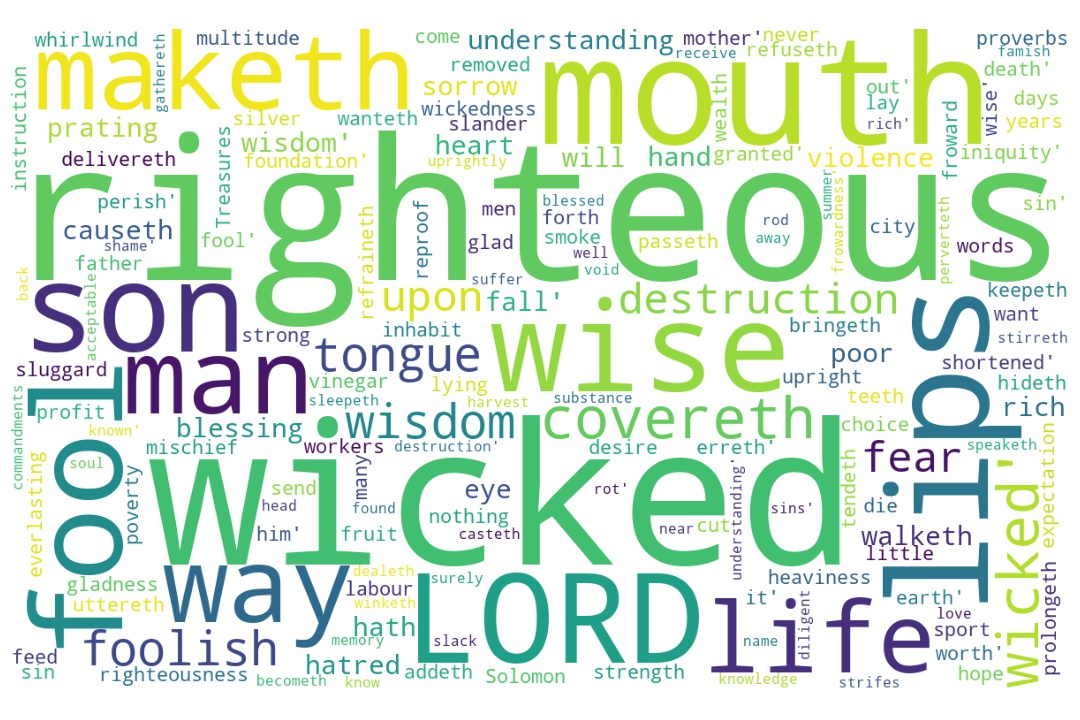
\includegraphics[width=\linewidth]{20OT-Proverbs/Proverb10-WordCloud.jpg}
  \caption{Proverb 10 Word Cloud}
  \label{fig:Proverb 10 Word Cloud}
\end{figure}

\marginpar{\scriptsize \centering\fcolorbox{bone}{lime}{\textbf{THE RIGHTEOUS \& WICKED}}\\ (Proverb 10:1-32)
\begin{compactenum}[I.][8]
	\item \textbf{Shame to the Lazy}  \index[scripture]{Proverbs!Pro 10:05} (Pro 10:5)
	\item \textbf{Sure Footing for the Upright}  \index[scripture]{Proverbs!Pro 10:09} (Pro 10:9)
	\item \textbf{Strife to the Hateful}  \index[scripture]{Proverbs!Pro 10:12} (Pro 10:12)
	\item More \textbf{Sin for the Wicked}  \index[scripture]{Proverbs!Pro 10:16} (Pro 10:16)
	\item \textbf{Sustenance form the Righteous}  \index[scripture]{Proverbs!Pro 10:21} (Pro 10:21)
	\item \textbf{Stinging Eyes to the Sluggard}  \index[scripture]{Proverbs!Pro 10:26} (Pro 10:26)
	\item \textbf{Strength to the Upright} \index[scripture]{Proverbs!Pro 10:29} (Pro 10:29)
\end{compactenum}}

\marginpar{\scriptsize \centering\fcolorbox{bone}{yellow}{\textbf{7 THINGS OF LIFE}}\\ (Proverb 10:1-32)
    \begin{compactenum}[I.][8]
	\item The \textbf{Well} of Life \index[scripture]{Proverbs!Pro 10:11} (Pro 10:11)
	
	\item A \textbf{Wellspring} of Life \index[scripture]{Proverbs!Pro 16:22} \index[scripture]{Proverbs!Pro 18:4} (Pro 16:22, 18:4)
	
	\item The \textbf{way} of Life \index[scripture]{Pro!Pro 06:23} \index[scripture]{Pro!Pro 10:17} \index[scripture]{Pro!Pro 15:24} \index[scripture]{Jer!Jer 21:8} (Pro 6:23, 10:17, 15:24, Jer 21:8)

	\item The \textbf{ways} of Life \index[scripture]{Acts!Acts 02:28} (Acts 2:28)
	
	\item The \textbf{water} of Life \index[scripture]{Rev!Rev 21:06} \index[scripture]{Rev!Rev 22:01} \index[scripture]{Rev!Rev 22:17}  (Rev 21:6, 22:1, 22:17)
	
	\item The \textbf{word} of Life \index[scripture]{Phil!Phil 02:16} (Phil 2:16)
	
	\item The \textbf{Word} of Life \index[scripture]{1Jn!1Jn 1:1}  (1 John 1:1)
\end{compactenum}}

\footnote{\textcolor[cmyk]{0.99998,1,0,0}{\hyperlink{TOC}{Return to end of Table of Contents.}}}\footnote{\href{https://audiobible.com/bible/proverbs_10.html}{\textcolor[cmyk]{0.99998,1,0,0}{Proverbs Audio}}}\textcolor[cmyk]{0.99998,1,0,0}{The proverbs of Solomon. A wise son maketh a glad father: but a foolish son \emph{is} the heaviness of his mother.}
[2] \textcolor[cmyk]{0.99998,1,0,0}{Treasures of wickedness profit nothing: but \fcolorbox{bone}{MYGOLD}{righteousness} delivereth from death.}
[3] \textcolor[cmyk]{0.99998,1,0,0}{The LORD will not suffer the soul of the righteous to famish: but he casteth away the substance of the wicked.}\footnote{\textbf{Psalm 37:25} - I have been young, and now am old; yet have I not seen the righteous forsaken, nor his seed begging bread.}
[4] \textcolor[cmyk]{0.99998,1,0,0}{He becometh poor that dealeth \emph{with} a slack hand: but the hand of the diligent maketh rich.}
[5] \textcolor[cmyk]{0.99998,1,0,0}{He that gathereth in summer \emph{is} a wise son: \emph{but} he that sleepeth in harvest \emph{is} a son that causeth \fcolorbox{bone}{lime}{shame}.}
[6] \textcolor[cmyk]{0.99998,1,0,0}{Blessings \emph{are} upon the head of the just: but violence covereth the mouth of the wicked.}
[7] \textcolor[cmyk]{0.99998,1,0,0}{The memory of the just \emph{is} blessed: but the name of the wicked shall rot.}
[8] \textcolor[cmyk]{0.99998,1,0,0}{Thewise in heart will receive commandments: but a prating fool shall fall.}
[9] \textcolor[cmyk]{0.99998,1,0,0}{He that walketh uprightly walketh \fcolorbox{bone}{lime}{surely}: but he that perverteth his ways shall be known.}
[10] \textcolor[cmyk]{0.99998,1,0,0}{He that winketh with the eye causeth sorrow: but a prating fool shall fall.}\footnote{\textbf{Proverbs 6:13} - He winketh with his eyes, he speaketh with his feet, he teacheth with his fingers;} 
[11] \textcolor[cmyk]{0.99998,1,0,0}{The mouth of a righteous \emph{man} \emph{is} a well of life: but violence covereth the mouth of the wicked.}\footnote{\textbf{Proverb 16:22} - Understanding is a wellspring of life unto him that hath it: but the instruction of fools is folly.}
[12] \textcolor[cmyk]{0.99998,1,0,0}{Hatred stirreth up \fcolorbox{bone}{lime}{strifes}: but love covereth all sins.}
[13] \textcolor[cmyk]{0.99998,1,0,0}{In  the lips of him that hath \fcolorbox{bone}{MYGOLD}{understanding} wisdom is found: but a rod \emph{is} for the back of him that is void of \fcolorbox{bone}{MYGOLD}{understanding}.}
[14] \textcolor[cmyk]{0.99998,1,0,0}{Wise  \emph{men} lay up knowledge: but the mouth of the foolish \emph{is} near destruction.}
[15] \textcolor[cmyk]{0.99998,1,0,0}{The  rich man's wealth \emph{is} his strong city: the destruction of the poor \emph{is} their poverty.}
[16] \textcolor[cmyk]{0.99998,1,0,0}{The  labour of the righteous \emph{tendeth} to life: the fruit of the wicked \fcolorbox{bone}{lime}{to sin}.}
[17] \textcolor[cmyk]{0.99998,1,0,0}{He  \emph{is} \emph{in} the way of life that keepeth instruction: but he that refuseth reproof erreth.}
[18] \textcolor[cmyk]{0.99998,1,0,0}{He  that hideth hatred \emph{with} lying lips, and he that uttereth a slander, \emph{is} a fool.}
[19] \textcolor[cmyk]{0.99998,1,0,0}{In  the multitude of words there wanteth not sin: but he that refraineth his lips \emph{is} wise.}
[20] \textcolor[cmyk]{0.99998,1,0,0}{The tongue of the just \emph{is} \emph{as} choice silver: the heart of the wicked \emph{is} little worth.}
[21] \textcolor[cmyk]{0.99998,1,0,0}{The lips of the righteous \fcolorbox{bone}{lime}{feed many}: but fools die for want of wisdom.}
[22] \textcolor[cmyk]{0.99998,1,0,0}{The blessing of the LORD, it maketh rich, and he addeth no sorrow with it.}
[23] \textcolor[cmyk]{0.99998,1,0,0}{\emph{It} \emph{is} as sport to a fool to do mischief: but a man of \fcolorbox{bone}{MYGOLD}{understanding} hath wisdom.}
[24] \textcolor[cmyk]{0.99998,1,0,0}{The fear of the wicked, it shall come upon him: but the desire of the righteous shall be granted.}
[25] \textcolor[cmyk]{0.99998,1,0,0}{As the whirlwind passeth, so \emph{is} the wicked no \emph{more}: but the righteous \emph{is} an everlasting foundation.}
[26] \textcolor[cmyk]{0.99998,1,0,0}{As vinegar to the teeth, and as \fcolorbox{bone}{lime}{smoke to the eyes}, so \emph{is} the sluggard to them that send him.}
[27] \textcolor[cmyk]{0.99998,1,0,0}{The fear of the LORD prolongeth days: but the years of the wicked shall be shortened.}
[28] \textcolor[cmyk]{0.99998,1,0,0}{The hope of the righteous \emph{shall} \emph{be} gladness: but the expectation of the wicked shall perish.}
[29] \textcolor[cmyk]{0.99998,1,0,0}{The way of the LORD \emph{is} \fcolorbox{bone}{lime}{strength to the upright}: but destruction \emph{shall} \emph{be} to the workers of iniquity.}
[30] \textcolor[cmyk]{0.99998,1,0,0}{The righteous shall never be removed: but the wicked shall not inhabit the earth.}
[31] \textcolor[cmyk]{0.99998,1,0,0}{The mouth of the just bringeth forth wisdom: but the froward tongue shall be cut out.}
[32] \textcolor[cmyk]{0.99998,1,0,0}{The lips of the righteous know what is acceptable: but the mouth of the wicked \emph{speaketh} frowardness.}


\index[NWIV]{21!Proverbs!Pro 10:1}\index[AWIP]{The!Proverbs!Pro 10:1}\index[AWIP]{proverbs!Proverbs!Pro 10:1}\index[AWIP]{of!Proverbs!Pro 10:1}\index[AWIP]{of!Proverbs!Pro 10:1 (2)}\index[AWIP]{Solomon!Proverbs!Pro 10:1}\index[AWIP]{A!Proverbs!Pro 10:1}\index[AWIP]{wise!Proverbs!Pro 10:1}\index[AWIP]{son!Proverbs!Pro 10:1}\index[AWIP]{son!Proverbs!Pro 10:1 (2)}\index[AWIP]{maketh!Proverbs!Pro 10:1}\index[AWIP]{a!Proverbs!Pro 10:1}\index[AWIP]{a!Proverbs!Pro 10:1 (2)}\index[AWIP]{glad!Proverbs!Pro 10:1}\index[AWIP]{father!Proverbs!Pro 10:1}\index[AWIP]{but!Proverbs!Pro 10:1}\index[AWIP]{foolish!Proverbs!Pro 10:1}\index[AWIP]{\emph{is}!Proverbs!Pro 10:1}\index[AWIP]{the!Proverbs!Pro 10:1}\index[AWIP]{heaviness!Proverbs!Pro 10:1}\index[AWIP]{his!Proverbs!Pro 10:1}\index[AWIP]{mother!Proverbs!Pro 10:1}\index[AWIP]{\emph{is}!Proverbs!Pro 10:1}

\index[NWIV]{10!Proverbs!Pro 10:2}\index[AWIP]{Treasures!Proverbs!Pro 10:2}\index[AWIP]{of!Proverbs!Pro 10:2}\index[AWIP]{wickedness!Proverbs!Pro 10:2}\index[AWIP]{profit!Proverbs!Pro 10:2}\index[AWIP]{nothing!Proverbs!Pro 10:2}\index[AWIP]{but!Proverbs!Pro 10:2}\index[AWIP]{righteousness!Proverbs!Pro 10:2}\index[AWIP]{delivereth!Proverbs!Pro 10:2}\index[AWIP]{from!Proverbs!Pro 10:2}\index[AWIP]{death!Proverbs!Pro 10:2}

\index[NWIV]{21!Proverbs!Pro 10:3}\index[AWIP]{The!Proverbs!Pro 10:3}\index[AWIP]{LORD!Proverbs!Pro 10:3}\index[AWIP]{will!Proverbs!Pro 10:3}\index[AWIP]{not!Proverbs!Pro 10:3}\index[AWIP]{suffer!Proverbs!Pro 10:3}\index[AWIP]{the!Proverbs!Pro 10:3}\index[AWIP]{the!Proverbs!Pro 10:3 (2)}\index[AWIP]{the!Proverbs!Pro 10:3 (3)}\index[AWIP]{the!Proverbs!Pro 10:3 (4)}\index[AWIP]{soul!Proverbs!Pro 10:3}\index[AWIP]{of!Proverbs!Pro 10:3}\index[AWIP]{of!Proverbs!Pro 10:3 (2)}\index[AWIP]{righteous!Proverbs!Pro 10:3}\index[AWIP]{to!Proverbs!Pro 10:3}\index[AWIP]{famish!Proverbs!Pro 10:3}\index[AWIP]{but!Proverbs!Pro 10:3}\index[AWIP]{he!Proverbs!Pro 10:3}\index[AWIP]{casteth!Proverbs!Pro 10:3}\index[AWIP]{away!Proverbs!Pro 10:3}\index[AWIP]{substance!Proverbs!Pro 10:3}\index[AWIP]{wicked!Proverbs!Pro 10:3}

\index[NWIV]{17!Proverbs!Pro 10:4}\index[AWIP]{He!Proverbs!Pro 10:4}\index[AWIP]{becometh!Proverbs!Pro 10:4}\index[AWIP]{poor!Proverbs!Pro 10:4}\index[AWIP]{that!Proverbs!Pro 10:4}\index[AWIP]{dealeth!Proverbs!Pro 10:4}\index[AWIP]{\emph{with}!Proverbs!Pro 10:4}\index[AWIP]{a!Proverbs!Pro 10:4}\index[AWIP]{slack!Proverbs!Pro 10:4}\index[AWIP]{hand!Proverbs!Pro 10:4}\index[AWIP]{hand!Proverbs!Pro 10:4 (2)}\index[AWIP]{but!Proverbs!Pro 10:4}\index[AWIP]{the!Proverbs!Pro 10:4}\index[AWIP]{the!Proverbs!Pro 10:4 (2)}\index[AWIP]{of!Proverbs!Pro 10:4}\index[AWIP]{diligent!Proverbs!Pro 10:4}\index[AWIP]{maketh!Proverbs!Pro 10:4}\index[AWIP]{rich!Proverbs!Pro 10:4}\index[AWIP]{\emph{with}!Proverbs!Pro 10:4}

\index[NWIV]{21!Proverbs!Pro 10:5}\index[AWIP]{He!Proverbs!Pro 10:5}\index[AWIP]{that!Proverbs!Pro 10:5}\index[AWIP]{that!Proverbs!Pro 10:5 (2)}\index[AWIP]{that!Proverbs!Pro 10:5 (3)}\index[AWIP]{gathereth!Proverbs!Pro 10:5}\index[AWIP]{in!Proverbs!Pro 10:5}\index[AWIP]{in!Proverbs!Pro 10:5 (2)}\index[AWIP]{summer!Proverbs!Pro 10:5}\index[AWIP]{\emph{is}!Proverbs!Pro 10:5}\index[AWIP]{\emph{is}!Proverbs!Pro 10:5 (2)}\index[AWIP]{a!Proverbs!Pro 10:5}\index[AWIP]{a!Proverbs!Pro 10:5 (2)}\index[AWIP]{wise!Proverbs!Pro 10:5}\index[AWIP]{son!Proverbs!Pro 10:5}\index[AWIP]{son!Proverbs!Pro 10:5 (2)}\index[AWIP]{\emph{but}!Proverbs!Pro 10:5}\index[AWIP]{he!Proverbs!Pro 10:5}\index[AWIP]{sleepeth!Proverbs!Pro 10:5}\index[AWIP]{harvest!Proverbs!Pro 10:5}\index[AWIP]{causeth!Proverbs!Pro 10:5}\index[AWIP]{shame!Proverbs!Pro 10:5}\index[AWIP]{\emph{is}!Proverbs!Pro 10:5}\index[AWIP]{\emph{is}!Proverbs!Pro 10:5 (2)}\index[AWIP]{\emph{but}!Proverbs!Pro 10:5}

\index[NWIV]{16!Proverbs!Pro 10:6}\index[AWIP]{Blessings!Proverbs!Pro 10:6}\index[AWIP]{\emph{are}!Proverbs!Pro 10:6}\index[AWIP]{upon!Proverbs!Pro 10:6}\index[AWIP]{the!Proverbs!Pro 10:6}\index[AWIP]{the!Proverbs!Pro 10:6 (2)}\index[AWIP]{the!Proverbs!Pro 10:6 (3)}\index[AWIP]{the!Proverbs!Pro 10:6 (4)}\index[AWIP]{head!Proverbs!Pro 10:6}\index[AWIP]{of!Proverbs!Pro 10:6}\index[AWIP]{of!Proverbs!Pro 10:6 (2)}\index[AWIP]{just!Proverbs!Pro 10:6}\index[AWIP]{but!Proverbs!Pro 10:6}\index[AWIP]{violence!Proverbs!Pro 10:6}\index[AWIP]{covereth!Proverbs!Pro 10:6}\index[AWIP]{mouth!Proverbs!Pro 10:6}\index[AWIP]{wicked!Proverbs!Pro 10:6}\index[AWIP]{\emph{are}!Proverbs!Pro 10:6}

\index[NWIV]{15!Proverbs!Pro 10:7}\index[AWIP]{The!Proverbs!Pro 10:7}\index[AWIP]{memory!Proverbs!Pro 10:7}\index[AWIP]{of!Proverbs!Pro 10:7}\index[AWIP]{of!Proverbs!Pro 10:7 (2)}\index[AWIP]{the!Proverbs!Pro 10:7}\index[AWIP]{the!Proverbs!Pro 10:7 (2)}\index[AWIP]{the!Proverbs!Pro 10:7 (3)}\index[AWIP]{just!Proverbs!Pro 10:7}\index[AWIP]{\emph{is}!Proverbs!Pro 10:7}\index[AWIP]{blessed!Proverbs!Pro 10:7}\index[AWIP]{but!Proverbs!Pro 10:7}\index[AWIP]{name!Proverbs!Pro 10:7}\index[AWIP]{wicked!Proverbs!Pro 10:7}\index[AWIP]{shall!Proverbs!Pro 10:7}\index[AWIP]{rot!Proverbs!Pro 10:7}\index[AWIP]{\emph{is}!Proverbs!Pro 10:7}

\index[NWIV]{13!Proverbs!Pro 10:8}\index[AWIP]{The!Proverbs!Pro 10:8}\index[AWIP]{wise!Proverbs!Pro 10:8}\index[AWIP]{in!Proverbs!Pro 10:8}\index[AWIP]{heart!Proverbs!Pro 10:8}\index[AWIP]{will!Proverbs!Pro 10:8}\index[AWIP]{receive!Proverbs!Pro 10:8}\index[AWIP]{commandments!Proverbs!Pro 10:8}\index[AWIP]{but!Proverbs!Pro 10:8}\index[AWIP]{a!Proverbs!Pro 10:8}\index[AWIP]{prating!Proverbs!Pro 10:8}\index[AWIP]{fool!Proverbs!Pro 10:8}\index[AWIP]{shall!Proverbs!Pro 10:8}\index[AWIP]{fall!Proverbs!Pro 10:8}

\index[NWIV]{15!Proverbs!Pro 10:9}\index[AWIP]{He!Proverbs!Pro 10:9}\index[AWIP]{that!Proverbs!Pro 10:9}\index[AWIP]{that!Proverbs!Pro 10:9 (2)}\index[AWIP]{walketh!Proverbs!Pro 10:9}\index[AWIP]{walketh!Proverbs!Pro 10:9 (2)}\index[AWIP]{uprightly!Proverbs!Pro 10:9}\index[AWIP]{surely!Proverbs!Pro 10:9}\index[AWIP]{but!Proverbs!Pro 10:9}\index[AWIP]{he!Proverbs!Pro 10:9}\index[AWIP]{perverteth!Proverbs!Pro 10:9}\index[AWIP]{his!Proverbs!Pro 10:9}\index[AWIP]{ways!Proverbs!Pro 10:9}\index[AWIP]{shall!Proverbs!Pro 10:9}\index[AWIP]{be!Proverbs!Pro 10:9}\index[AWIP]{known!Proverbs!Pro 10:9}

\index[NWIV]{14!Proverbs!Pro 10:10}\index[AWIP]{He!Proverbs!Pro 10:10}\index[AWIP]{that!Proverbs!Pro 10:10}\index[AWIP]{winketh!Proverbs!Pro 10:10}\index[AWIP]{with!Proverbs!Pro 10:10}\index[AWIP]{the!Proverbs!Pro 10:10}\index[AWIP]{eye!Proverbs!Pro 10:10}\index[AWIP]{causeth!Proverbs!Pro 10:10}\index[AWIP]{sorrow!Proverbs!Pro 10:10}\index[AWIP]{but!Proverbs!Pro 10:10}\index[AWIP]{a!Proverbs!Pro 10:10}\index[AWIP]{prating!Proverbs!Pro 10:10}\index[AWIP]{fool!Proverbs!Pro 10:10}\index[AWIP]{shall!Proverbs!Pro 10:10}\index[AWIP]{fall!Proverbs!Pro 10:10}

\index[NWIV]{19!Proverbs!Pro 10:11}\index[AWIP]{The!Proverbs!Pro 10:11}\index[AWIP]{mouth!Proverbs!Pro 10:11}\index[AWIP]{mouth!Proverbs!Pro 10:11 (2)}\index[AWIP]{of!Proverbs!Pro 10:11}\index[AWIP]{of!Proverbs!Pro 10:11 (2)}\index[AWIP]{of!Proverbs!Pro 10:11 (3)}\index[AWIP]{a!Proverbs!Pro 10:11}\index[AWIP]{a!Proverbs!Pro 10:11 (2)}\index[AWIP]{righteous!Proverbs!Pro 10:11}\index[AWIP]{\emph{man}!Proverbs!Pro 10:11}\index[AWIP]{\emph{is}!Proverbs!Pro 10:11}\index[AWIP]{well!Proverbs!Pro 10:11}\index[AWIP]{life!Proverbs!Pro 10:11}\index[AWIP]{but!Proverbs!Pro 10:11}\index[AWIP]{violence!Proverbs!Pro 10:11}\index[AWIP]{covereth!Proverbs!Pro 10:11}\index[AWIP]{the!Proverbs!Pro 10:11}\index[AWIP]{the!Proverbs!Pro 10:11 (2)}\index[AWIP]{wicked!Proverbs!Pro 10:11}\index[AWIP]{\emph{man}!Proverbs!Pro 10:11}\index[AWIP]{\emph{is}!Proverbs!Pro 10:11}

\index[NWIV]{9!Proverbs!Pro 10:12}\index[AWIP]{Hatred!Proverbs!Pro 10:12}\index[AWIP]{stirreth!Proverbs!Pro 10:12}\index[AWIP]{up!Proverbs!Pro 10:12}\index[AWIP]{strifes!Proverbs!Pro 10:12}\index[AWIP]{but!Proverbs!Pro 10:12}\index[AWIP]{love!Proverbs!Pro 10:12}\index[AWIP]{covereth!Proverbs!Pro 10:12}\index[AWIP]{all!Proverbs!Pro 10:12}\index[AWIP]{sins!Proverbs!Pro 10:12}

\index[NWIV]{25!Proverbs!Pro 10:13}\index[AWIP]{In!Proverbs!Pro 10:13}\index[AWIP]{the!Proverbs!Pro 10:13}\index[AWIP]{the!Proverbs!Pro 10:13 (2)}\index[AWIP]{lips!Proverbs!Pro 10:13}\index[AWIP]{of!Proverbs!Pro 10:13}\index[AWIP]{of!Proverbs!Pro 10:13 (2)}\index[AWIP]{of!Proverbs!Pro 10:13 (3)}\index[AWIP]{him!Proverbs!Pro 10:13}\index[AWIP]{him!Proverbs!Pro 10:13 (2)}\index[AWIP]{that!Proverbs!Pro 10:13}\index[AWIP]{that!Proverbs!Pro 10:13 (2)}\index[AWIP]{hath!Proverbs!Pro 10:13}\index[AWIP]{understanding!Proverbs!Pro 10:13}\index[AWIP]{understanding!Proverbs!Pro 10:13 (2)}\index[AWIP]{wisdom!Proverbs!Pro 10:13}\index[AWIP]{is!Proverbs!Pro 10:13}\index[AWIP]{is!Proverbs!Pro 10:13 (2)}\index[AWIP]{found!Proverbs!Pro 10:13}\index[AWIP]{but!Proverbs!Pro 10:13}\index[AWIP]{a!Proverbs!Pro 10:13}\index[AWIP]{rod!Proverbs!Pro 10:13}\index[AWIP]{\emph{is}!Proverbs!Pro 10:13}\index[AWIP]{for!Proverbs!Pro 10:13}\index[AWIP]{back!Proverbs!Pro 10:13}\index[AWIP]{void!Proverbs!Pro 10:13}\index[AWIP]{\emph{is}!Proverbs!Pro 10:13}

\index[NWIV]{14!Proverbs!Pro 10:14}\index[AWIP]{Wise!Proverbs!Pro 10:14}\index[AWIP]{\emph{men}!Proverbs!Pro 10:14}\index[AWIP]{lay!Proverbs!Pro 10:14}\index[AWIP]{up!Proverbs!Pro 10:14}\index[AWIP]{knowledge!Proverbs!Pro 10:14}\index[AWIP]{but!Proverbs!Pro 10:14}\index[AWIP]{the!Proverbs!Pro 10:14}\index[AWIP]{the!Proverbs!Pro 10:14 (2)}\index[AWIP]{mouth!Proverbs!Pro 10:14}\index[AWIP]{of!Proverbs!Pro 10:14}\index[AWIP]{foolish!Proverbs!Pro 10:14}\index[AWIP]{\emph{is}!Proverbs!Pro 10:14}\index[AWIP]{near!Proverbs!Pro 10:14}\index[AWIP]{destruction!Proverbs!Pro 10:14}\index[AWIP]{\emph{men}!Proverbs!Pro 10:14}\index[AWIP]{\emph{is}!Proverbs!Pro 10:14}

\index[NWIV]{16!Proverbs!Pro 10:15}\index[AWIP]{The!Proverbs!Pro 10:15}\index[AWIP]{rich!Proverbs!Pro 10:15}\index[AWIP]{man's!Proverbs!Pro 10:15}\index[AWIP]{wealth!Proverbs!Pro 10:15}\index[AWIP]{\emph{is}!Proverbs!Pro 10:15}\index[AWIP]{\emph{is}!Proverbs!Pro 10:15 (2)}\index[AWIP]{his!Proverbs!Pro 10:15}\index[AWIP]{strong!Proverbs!Pro 10:15}\index[AWIP]{city!Proverbs!Pro 10:15}\index[AWIP]{the!Proverbs!Pro 10:15}\index[AWIP]{the!Proverbs!Pro 10:15 (2)}\index[AWIP]{destruction!Proverbs!Pro 10:15}\index[AWIP]{of!Proverbs!Pro 10:15}\index[AWIP]{poor!Proverbs!Pro 10:15}\index[AWIP]{their!Proverbs!Pro 10:15}\index[AWIP]{poverty!Proverbs!Pro 10:15}\index[AWIP]{\emph{is}!Proverbs!Pro 10:15}\index[AWIP]{\emph{is}!Proverbs!Pro 10:15 (2)}

\index[NWIV]{15!Proverbs!Pro 10:16}\index[AWIP]{The!Proverbs!Pro 10:16}\index[AWIP]{labour!Proverbs!Pro 10:16}\index[AWIP]{of!Proverbs!Pro 10:16}\index[AWIP]{of!Proverbs!Pro 10:16 (2)}\index[AWIP]{the!Proverbs!Pro 10:16}\index[AWIP]{the!Proverbs!Pro 10:16 (2)}\index[AWIP]{the!Proverbs!Pro 10:16 (3)}\index[AWIP]{righteous!Proverbs!Pro 10:16}\index[AWIP]{\emph{tendeth}!Proverbs!Pro 10:16}\index[AWIP]{to!Proverbs!Pro 10:16}\index[AWIP]{to!Proverbs!Pro 10:16 (2)}\index[AWIP]{life!Proverbs!Pro 10:16}\index[AWIP]{fruit!Proverbs!Pro 10:16}\index[AWIP]{wicked!Proverbs!Pro 10:16}\index[AWIP]{sin!Proverbs!Pro 10:16}\index[AWIP]{\emph{tendeth}!Proverbs!Pro 10:16}

\index[NWIV]{16!Proverbs!Pro 10:17}\index[AWIP]{He!Proverbs!Pro 10:17}\index[AWIP]{\emph{is}!Proverbs!Pro 10:17}\index[AWIP]{\emph{in}!Proverbs!Pro 10:17}\index[AWIP]{the!Proverbs!Pro 10:17}\index[AWIP]{way!Proverbs!Pro 10:17}\index[AWIP]{of!Proverbs!Pro 10:17}\index[AWIP]{life!Proverbs!Pro 10:17}\index[AWIP]{that!Proverbs!Pro 10:17}\index[AWIP]{that!Proverbs!Pro 10:17 (2)}\index[AWIP]{keepeth!Proverbs!Pro 10:17}\index[AWIP]{instruction!Proverbs!Pro 10:17}\index[AWIP]{but!Proverbs!Pro 10:17}\index[AWIP]{he!Proverbs!Pro 10:17}\index[AWIP]{refuseth!Proverbs!Pro 10:17}\index[AWIP]{reproof!Proverbs!Pro 10:17}\index[AWIP]{erreth!Proverbs!Pro 10:17}\index[AWIP]{\emph{is}!Proverbs!Pro 10:17}\index[AWIP]{\emph{in}!Proverbs!Pro 10:17}

\index[NWIV]{16!Proverbs!Pro 10:18}\index[AWIP]{He!Proverbs!Pro 10:18}\index[AWIP]{that!Proverbs!Pro 10:18}\index[AWIP]{that!Proverbs!Pro 10:18 (2)}\index[AWIP]{hideth!Proverbs!Pro 10:18}\index[AWIP]{hatred!Proverbs!Pro 10:18}\index[AWIP]{\emph{with}!Proverbs!Pro 10:18}\index[AWIP]{lying!Proverbs!Pro 10:18}\index[AWIP]{lips!Proverbs!Pro 10:18}\index[AWIP]{and!Proverbs!Pro 10:18}\index[AWIP]{he!Proverbs!Pro 10:18}\index[AWIP]{uttereth!Proverbs!Pro 10:18}\index[AWIP]{a!Proverbs!Pro 10:18}\index[AWIP]{a!Proverbs!Pro 10:18 (2)}\index[AWIP]{slander!Proverbs!Pro 10:18}\index[AWIP]{\emph{is}!Proverbs!Pro 10:18}\index[AWIP]{fool!Proverbs!Pro 10:18}\index[AWIP]{\emph{with}!Proverbs!Pro 10:18}\index[AWIP]{\emph{is}!Proverbs!Pro 10:18}

\index[NWIV]{17!Proverbs!Pro 10:19}\index[AWIP]{In!Proverbs!Pro 10:19}\index[AWIP]{the!Proverbs!Pro 10:19}\index[AWIP]{multitude!Proverbs!Pro 10:19}\index[AWIP]{of!Proverbs!Pro 10:19}\index[AWIP]{words!Proverbs!Pro 10:19}\index[AWIP]{there!Proverbs!Pro 10:19}\index[AWIP]{wanteth!Proverbs!Pro 10:19}\index[AWIP]{not!Proverbs!Pro 10:19}\index[AWIP]{sin!Proverbs!Pro 10:19}\index[AWIP]{but!Proverbs!Pro 10:19}\index[AWIP]{he!Proverbs!Pro 10:19}\index[AWIP]{that!Proverbs!Pro 10:19}\index[AWIP]{refraineth!Proverbs!Pro 10:19}\index[AWIP]{his!Proverbs!Pro 10:19}\index[AWIP]{lips!Proverbs!Pro 10:19}\index[AWIP]{\emph{is}!Proverbs!Pro 10:19}\index[AWIP]{wise!Proverbs!Pro 10:19}\index[AWIP]{\emph{is}!Proverbs!Pro 10:19}

\index[NWIV]{17!Proverbs!Pro 10:20}\index[AWIP]{The!Proverbs!Pro 10:20}\index[AWIP]{tongue!Proverbs!Pro 10:20}\index[AWIP]{of!Proverbs!Pro 10:20}\index[AWIP]{of!Proverbs!Pro 10:20 (2)}\index[AWIP]{the!Proverbs!Pro 10:20}\index[AWIP]{the!Proverbs!Pro 10:20 (2)}\index[AWIP]{the!Proverbs!Pro 10:20 (3)}\index[AWIP]{just!Proverbs!Pro 10:20}\index[AWIP]{\emph{is}!Proverbs!Pro 10:20}\index[AWIP]{\emph{is}!Proverbs!Pro 10:20 (2)}\index[AWIP]{\emph{as}!Proverbs!Pro 10:20}\index[AWIP]{choice!Proverbs!Pro 10:20}\index[AWIP]{silver!Proverbs!Pro 10:20}\index[AWIP]{heart!Proverbs!Pro 10:20}\index[AWIP]{wicked!Proverbs!Pro 10:20}\index[AWIP]{little!Proverbs!Pro 10:20}\index[AWIP]{worth!Proverbs!Pro 10:20}\index[AWIP]{\emph{is}!Proverbs!Pro 10:20}\index[AWIP]{\emph{is}!Proverbs!Pro 10:20 (2)}\index[AWIP]{\emph{as}!Proverbs!Pro 10:20}

\index[NWIV]{14!Proverbs!Pro 10:21}\index[AWIP]{The!Proverbs!Pro 10:21}\index[AWIP]{lips!Proverbs!Pro 10:21}\index[AWIP]{of!Proverbs!Pro 10:21}\index[AWIP]{of!Proverbs!Pro 10:21 (2)}\index[AWIP]{the!Proverbs!Pro 10:21}\index[AWIP]{righteous!Proverbs!Pro 10:21}\index[AWIP]{feed!Proverbs!Pro 10:21}\index[AWIP]{many!Proverbs!Pro 10:21}\index[AWIP]{but!Proverbs!Pro 10:21}\index[AWIP]{fools!Proverbs!Pro 10:21}\index[AWIP]{die!Proverbs!Pro 10:21}\index[AWIP]{for!Proverbs!Pro 10:21}\index[AWIP]{want!Proverbs!Pro 10:21}\index[AWIP]{wisdom!Proverbs!Pro 10:21}

\index[NWIV]{15!Proverbs!Pro 10:22}\index[AWIP]{The!Proverbs!Pro 10:22}\index[AWIP]{blessing!Proverbs!Pro 10:22}\index[AWIP]{of!Proverbs!Pro 10:22}\index[AWIP]{the!Proverbs!Pro 10:22}\index[AWIP]{LORD!Proverbs!Pro 10:22}\index[AWIP]{it!Proverbs!Pro 10:22}\index[AWIP]{it!Proverbs!Pro 10:22 (2)}\index[AWIP]{maketh!Proverbs!Pro 10:22}\index[AWIP]{rich!Proverbs!Pro 10:22}\index[AWIP]{and!Proverbs!Pro 10:22}\index[AWIP]{he!Proverbs!Pro 10:22}\index[AWIP]{addeth!Proverbs!Pro 10:22}\index[AWIP]{no!Proverbs!Pro 10:22}\index[AWIP]{sorrow!Proverbs!Pro 10:22}\index[AWIP]{with!Proverbs!Pro 10:22}

\index[NWIV]{17!Proverbs!Pro 10:23}\index[AWIP]{\emph{It}!Proverbs!Pro 10:23}\index[AWIP]{\emph{is}!Proverbs!Pro 10:23}\index[AWIP]{as!Proverbs!Pro 10:23}\index[AWIP]{sport!Proverbs!Pro 10:23}\index[AWIP]{to!Proverbs!Pro 10:23}\index[AWIP]{to!Proverbs!Pro 10:23 (2)}\index[AWIP]{a!Proverbs!Pro 10:23}\index[AWIP]{a!Proverbs!Pro 10:23 (2)}\index[AWIP]{fool!Proverbs!Pro 10:23}\index[AWIP]{do!Proverbs!Pro 10:23}\index[AWIP]{mischief!Proverbs!Pro 10:23}\index[AWIP]{but!Proverbs!Pro 10:23}\index[AWIP]{man!Proverbs!Pro 10:23}\index[AWIP]{of!Proverbs!Pro 10:23}\index[AWIP]{understanding!Proverbs!Pro 10:23}\index[AWIP]{hath!Proverbs!Pro 10:23}\index[AWIP]{wisdom!Proverbs!Pro 10:23}\index[AWIP]{\emph{It}!Proverbs!Pro 10:23}\index[AWIP]{\emph{is}!Proverbs!Pro 10:23}

\index[NWIV]{19!Proverbs!Pro 10:24}\index[AWIP]{The!Proverbs!Pro 10:24}\index[AWIP]{fear!Proverbs!Pro 10:24}\index[AWIP]{of!Proverbs!Pro 10:24}\index[AWIP]{of!Proverbs!Pro 10:24 (2)}\index[AWIP]{the!Proverbs!Pro 10:24}\index[AWIP]{the!Proverbs!Pro 10:24 (2)}\index[AWIP]{the!Proverbs!Pro 10:24 (3)}\index[AWIP]{wicked!Proverbs!Pro 10:24}\index[AWIP]{it!Proverbs!Pro 10:24}\index[AWIP]{shall!Proverbs!Pro 10:24}\index[AWIP]{shall!Proverbs!Pro 10:24 (2)}\index[AWIP]{come!Proverbs!Pro 10:24}\index[AWIP]{upon!Proverbs!Pro 10:24}\index[AWIP]{him!Proverbs!Pro 10:24}\index[AWIP]{but!Proverbs!Pro 10:24}\index[AWIP]{desire!Proverbs!Pro 10:24}\index[AWIP]{righteous!Proverbs!Pro 10:24}\index[AWIP]{be!Proverbs!Pro 10:24}\index[AWIP]{granted!Proverbs!Pro 10:24}

\index[NWIV]{17!Proverbs!Pro 10:25}\index[AWIP]{As!Proverbs!Pro 10:25}\index[AWIP]{the!Proverbs!Pro 10:25}\index[AWIP]{the!Proverbs!Pro 10:25 (2)}\index[AWIP]{the!Proverbs!Pro 10:25 (3)}\index[AWIP]{whirlwind!Proverbs!Pro 10:25}\index[AWIP]{passeth!Proverbs!Pro 10:25}\index[AWIP]{so!Proverbs!Pro 10:25}\index[AWIP]{\emph{is}!Proverbs!Pro 10:25}\index[AWIP]{\emph{is}!Proverbs!Pro 10:25 (2)}\index[AWIP]{wicked!Proverbs!Pro 10:25}\index[AWIP]{no!Proverbs!Pro 10:25}\index[AWIP]{\emph{more}!Proverbs!Pro 10:25}\index[AWIP]{but!Proverbs!Pro 10:25}\index[AWIP]{righteous!Proverbs!Pro 10:25}\index[AWIP]{an!Proverbs!Pro 10:25}\index[AWIP]{everlasting!Proverbs!Pro 10:25}\index[AWIP]{foundation!Proverbs!Pro 10:25}\index[AWIP]{\emph{is}!Proverbs!Pro 10:25}\index[AWIP]{\emph{is}!Proverbs!Pro 10:25 (2)}\index[AWIP]{\emph{more}!Proverbs!Pro 10:25}

\index[NWIV]{20!Proverbs!Pro 10:26}\index[AWIP]{As!Proverbs!Pro 10:26}\index[AWIP]{vinegar!Proverbs!Pro 10:26}\index[AWIP]{to!Proverbs!Pro 10:26}\index[AWIP]{to!Proverbs!Pro 10:26 (2)}\index[AWIP]{to!Proverbs!Pro 10:26 (3)}\index[AWIP]{the!Proverbs!Pro 10:26}\index[AWIP]{the!Proverbs!Pro 10:26 (2)}\index[AWIP]{the!Proverbs!Pro 10:26 (3)}\index[AWIP]{teeth!Proverbs!Pro 10:26}\index[AWIP]{and!Proverbs!Pro 10:26}\index[AWIP]{as!Proverbs!Pro 10:26}\index[AWIP]{smoke!Proverbs!Pro 10:26}\index[AWIP]{eyes!Proverbs!Pro 10:26}\index[AWIP]{so!Proverbs!Pro 10:26}\index[AWIP]{\emph{is}!Proverbs!Pro 10:26}\index[AWIP]{sluggard!Proverbs!Pro 10:26}\index[AWIP]{them!Proverbs!Pro 10:26}\index[AWIP]{that!Proverbs!Pro 10:26}\index[AWIP]{send!Proverbs!Pro 10:26}\index[AWIP]{him!Proverbs!Pro 10:26}\index[AWIP]{\emph{is}!Proverbs!Pro 10:26}

\index[NWIV]{16!Proverbs!Pro 10:27}\index[AWIP]{The!Proverbs!Pro 10:27}\index[AWIP]{fear!Proverbs!Pro 10:27}\index[AWIP]{of!Proverbs!Pro 10:27}\index[AWIP]{of!Proverbs!Pro 10:27 (2)}\index[AWIP]{the!Proverbs!Pro 10:27}\index[AWIP]{the!Proverbs!Pro 10:27 (2)}\index[AWIP]{the!Proverbs!Pro 10:27 (3)}\index[AWIP]{LORD!Proverbs!Pro 10:27}\index[AWIP]{prolongeth!Proverbs!Pro 10:27}\index[AWIP]{days!Proverbs!Pro 10:27}\index[AWIP]{but!Proverbs!Pro 10:27}\index[AWIP]{years!Proverbs!Pro 10:27}\index[AWIP]{wicked!Proverbs!Pro 10:27}\index[AWIP]{shall!Proverbs!Pro 10:27}\index[AWIP]{be!Proverbs!Pro 10:27}\index[AWIP]{shortened!Proverbs!Pro 10:27}

\index[NWIV]{16!Proverbs!Pro 10:28}\index[AWIP]{The!Proverbs!Pro 10:28}\index[AWIP]{hope!Proverbs!Pro 10:28}\index[AWIP]{of!Proverbs!Pro 10:28}\index[AWIP]{of!Proverbs!Pro 10:28 (2)}\index[AWIP]{the!Proverbs!Pro 10:28}\index[AWIP]{the!Proverbs!Pro 10:28 (2)}\index[AWIP]{the!Proverbs!Pro 10:28 (3)}\index[AWIP]{righteous!Proverbs!Pro 10:28}\index[AWIP]{\emph{shall}!Proverbs!Pro 10:28}\index[AWIP]{\emph{be}!Proverbs!Pro 10:28}\index[AWIP]{gladness!Proverbs!Pro 10:28}\index[AWIP]{but!Proverbs!Pro 10:28}\index[AWIP]{expectation!Proverbs!Pro 10:28}\index[AWIP]{wicked!Proverbs!Pro 10:28}\index[AWIP]{shall!Proverbs!Pro 10:28}\index[AWIP]{perish!Proverbs!Pro 10:28}\index[AWIP]{\emph{shall}!Proverbs!Pro 10:28}\index[AWIP]{\emph{be}!Proverbs!Pro 10:28}

\index[NWIV]{19!Proverbs!Pro 10:29}\index[AWIP]{The!Proverbs!Pro 10:29}\index[AWIP]{way!Proverbs!Pro 10:29}\index[AWIP]{of!Proverbs!Pro 10:29}\index[AWIP]{of!Proverbs!Pro 10:29 (2)}\index[AWIP]{the!Proverbs!Pro 10:29}\index[AWIP]{the!Proverbs!Pro 10:29 (2)}\index[AWIP]{the!Proverbs!Pro 10:29 (3)}\index[AWIP]{LORD!Proverbs!Pro 10:29}\index[AWIP]{\emph{is}!Proverbs!Pro 10:29}\index[AWIP]{strength!Proverbs!Pro 10:29}\index[AWIP]{to!Proverbs!Pro 10:29}\index[AWIP]{to!Proverbs!Pro 10:29 (2)}\index[AWIP]{upright!Proverbs!Pro 10:29}\index[AWIP]{but!Proverbs!Pro 10:29}\index[AWIP]{destruction!Proverbs!Pro 10:29}\index[AWIP]{\emph{shall}!Proverbs!Pro 10:29}\index[AWIP]{\emph{be}!Proverbs!Pro 10:29}\index[AWIP]{workers!Proverbs!Pro 10:29}\index[AWIP]{iniquity!Proverbs!Pro 10:29}\index[AWIP]{\emph{is}!Proverbs!Pro 10:29}\index[AWIP]{\emph{shall}!Proverbs!Pro 10:29}\index[AWIP]{\emph{be}!Proverbs!Pro 10:29}

\index[NWIV]{14!Proverbs!Pro 10:30}\index[AWIP]{The!Proverbs!Pro 10:30}\index[AWIP]{righteous!Proverbs!Pro 10:30}\index[AWIP]{shall!Proverbs!Pro 10:30}\index[AWIP]{shall!Proverbs!Pro 10:30 (2)}\index[AWIP]{never!Proverbs!Pro 10:30}\index[AWIP]{be!Proverbs!Pro 10:30}\index[AWIP]{removed!Proverbs!Pro 10:30}\index[AWIP]{but!Proverbs!Pro 10:30}\index[AWIP]{the!Proverbs!Pro 10:30}\index[AWIP]{the!Proverbs!Pro 10:30 (2)}\index[AWIP]{wicked!Proverbs!Pro 10:30}\index[AWIP]{not!Proverbs!Pro 10:30}\index[AWIP]{inhabit!Proverbs!Pro 10:30}\index[AWIP]{earth!Proverbs!Pro 10:30}

\index[NWIV]{16!Proverbs!Pro 10:31}\index[AWIP]{The!Proverbs!Pro 10:31}\index[AWIP]{mouth!Proverbs!Pro 10:31}\index[AWIP]{of!Proverbs!Pro 10:31}\index[AWIP]{the!Proverbs!Pro 10:31}\index[AWIP]{the!Proverbs!Pro 10:31 (2)}\index[AWIP]{just!Proverbs!Pro 10:31}\index[AWIP]{bringeth!Proverbs!Pro 10:31}\index[AWIP]{forth!Proverbs!Pro 10:31}\index[AWIP]{wisdom!Proverbs!Pro 10:31}\index[AWIP]{but!Proverbs!Pro 10:31}\index[AWIP]{froward!Proverbs!Pro 10:31}\index[AWIP]{tongue!Proverbs!Pro 10:31}\index[AWIP]{shall!Proverbs!Pro 10:31}\index[AWIP]{be!Proverbs!Pro 10:31}\index[AWIP]{cut!Proverbs!Pro 10:31}\index[AWIP]{out!Proverbs!Pro 10:31}

\index[NWIV]{17!Proverbs!Pro 10:32}\index[AWIP]{The!Proverbs!Pro 10:32}\index[AWIP]{lips!Proverbs!Pro 10:32}\index[AWIP]{of!Proverbs!Pro 10:32}\index[AWIP]{of!Proverbs!Pro 10:32 (2)}\index[AWIP]{the!Proverbs!Pro 10:32}\index[AWIP]{the!Proverbs!Pro 10:32 (2)}\index[AWIP]{the!Proverbs!Pro 10:32 (3)}\index[AWIP]{righteous!Proverbs!Pro 10:32}\index[AWIP]{know!Proverbs!Pro 10:32}\index[AWIP]{what!Proverbs!Pro 10:32}\index[AWIP]{is!Proverbs!Pro 10:32}\index[AWIP]{acceptable!Proverbs!Pro 10:32}\index[AWIP]{but!Proverbs!Pro 10:32}\index[AWIP]{mouth!Proverbs!Pro 10:32}\index[AWIP]{wicked!Proverbs!Pro 10:32}\index[AWIP]{\emph{speaketh}!Proverbs!Pro 10:32}\index[AWIP]{frowardness!Proverbs!Pro 10:32}\index[AWIP]{\emph{speaketh}!Proverbs!Pro 10:32}

%%%%%%%%%%%%%%%%%%%%%%

\index[DOCTRINES]{Practicology - Substance!!Proverbs!Pro 10:02}
\index[DOCTRINES]{Practicology - Substance!!Proverbs!Pro 10:03}


\index[DOCTRINES]{Practicology - Strife!!Proverbs!Pro 10:12}

\index[DOCTRINES]{Practicology - Success!!Proverbs!Pro 10:16}


\index[DOCTRINES]{Practicology - Speech!!Proverbs!Pro 10:21}







\section{Proverbs 10 Outlines}

\subsection{Outlines from Others}

\subsubsection{Comparing the Righteous and Wicked}
\index[speaker]{Keith Anthony!Proverb 10 (Comparing the Righteous and Wicked)}
\index[series]{Proverbs (Keith Anthony)!Pro 10 (Comparing the Righteous and Wicked)}
\index[date]{2016/05/10!Proverb 10 (Comparing the Righteous and Wicked) (Keith Anthony)}
%\textbf{Lineage}: adpated from S. Conway\\
\textbf{Introduction}: Proverbs 10 begins a section of Solomon's proverbs comparing the righteous and wicked. There is:
\begin{compactenum}[I.]
\item \textbf{Shame to the Lazy}  \index[scripture]{Proverbs!Pro 10:05}(Pro 10:5)
\item \textbf{Sure Footing for the Upright}  \index[scripture]{Proverbs!Pro 10:09}(Pro 10:9)
\item \textbf{Strife to the Hateful}  \index[scripture]{Proverbs!Pro 10:12}(Pro 10:12)
\item More \textbf{Sin for the Wicked}  \index[scripture]{Proverbs!Pro 10:16}(Pro 10:16)
\item \textbf{Sustenance form the Righteous}  \index[scripture]{Proverbs!Pro 10:21}(Pro 10:21)
\item \textbf{Stinging Eyes to the Sluggard}  \index[scripture]{Proverbs!Pro 10:26}(Pro 10:26)
\item \textbf{Strength to the Upright} \index[scripture]{Proverbs!Pro 10:29}(Pro 10:29)
\end{compactenum}

% wisdom [1, 5, 19], wicked [2, 3, 6, 7, 11, 16, 20, 24, 25, 27, 28, 30, 32], walk, wink [10], whirlwind [5], way [17, 29], wealth [10], well [10], worth [20]
\subsection{Outlines from Others}


\section{Proverb 10 Comments}

\subsection{Numeric Nuggets}
\textbf{13:} There are 13 words in Proverb 10:8. Verses 8, 9, 14, 20, 21, 27, and 28 have 13 unique words. The 13-letter words in the chapter are ``righteousness'' and ``understanding.''  





%%% For Indexes

%\index[DEVOTIONAL]{TGIF1!Os Hillman (Living for a Cause Greater Than Yourself) - Proverb 19:17!2021/12/21}

%\index[DEVOTIONAL]{TGIF1!Os Hillman (Living for a Cause Greater Than Yourself) - Proverb 19:17!2021/12/21}

















%%% colour: cardinal red - \textcolor[cmyk]{0,0.85,0.70,0.23}{text}


%%%% Example marginpar with a compactenum list --- green color text
%\marginpar{\scriptsize \textcolor[rgb]{0.00,0.545,0.269}{$\rightarrow$7 Abominations: 
%\begin{compactenum}
%	\item A proud look,
%	\item a lying tongue,
%	\item hands that shed innocent blood,
%	\item An heart that deviseth wicked imaginations,
%	\item feet that be swift in running to mischief,
%	\item A false witness that speaketh lies, and
%	\item he that soweth discord among brethren.
%\end{compactenum}}}



%\newpage

%\begin{mdframed}[style=MyFrame]
%\begin{center}
%\begin{longtable}{|p{.5in}|p{3.5in}|}

%\caption[Corruption Alert: Proverbs 18:1]{Corruption Alert: Proverbs 18:1} \label{table:CorruptionProv18:1} \\ 

%\hline  
%\multicolumn{1}{|c|}{\textbf{Version}} & 
%\multicolumn{1}{c|}{\textbf{Corruption}}  \\ \hline 
%\endfirsthead
 
%\multicolumn{2}{c}
%{{\bfseries \tablename\ \thetable{} -- continued from previous page}} \\  \hline  
%\multicolumn{1}{|c|}{\textbf{Version}} & 
%\multicolumn{1}{c|}{\textbf{Corruption}}  \\ \hline 
%\endhead
 
%\hline \multicolumn{2}{|r|}{{Continued on next page}} \\ \hline
%\endfoot 
%\textcolor[rgb]{0.00,0.00,1.00}{AV} & \textcolor[rgb]{0.00,0.00,1.00}{Through desire a man, having separated himself, seeketh \emph{and} intermeddleth with all wisdom.} \\ \hline
%
%ASV &  He that separateth himself seeketh his own desire, And  rageth against all sound wisdom. \\ \hline
%
%CEB &  Unfriendly people look out for themselves; they bicker with sensible people.\\ \hline
%
%ESV & Whoever isolates himself seeks his own desire;  he breaks out against all sound judgment. \\ \hline
%
%NASV &  He who separates himself seeks his own desire, He quarrels against all sound wisdom.\\ \hline
%
%MEV & He who separates himself seeks his own desire; he seeks and quarrels against all wisdom.\\ \hline
%
%NIV &  An unfriendly person pursues selfish ends and against all sound judgment starts quarrels. \\ \hline
%
%NKJV &  A man who isolates himself seeks his own desire; He rages against all wise judgment.\\ \hline
%
%RSV &  He who is estranged seeks pretexts  to break out against all sound judgment.\\ \hline

% \multicolumn{2}{p{4.3in}}{{Modern translations, such as the ASV and others, strike out the first part of the verse, concealing the intent of mankind in genewisdom clearly revealed in scripture. How wonderful is the obfuscated RSV text: ``He who is estranged seeks pretexts.'' What does THAT mean?}} \\ %\hline

%\hline

%\end{longtable}
%\end{center}

%\normalsize 
%\end{mdframed}

%\marginpar{\scriptsize \centering \fcolorbox{black}{lime}{\textbf{OUTIDE THE PLACE OF PROMISE}}\\ (Psalm 137:1--9) 
%\begin{compactenum}[I.][8]
%	\item \textbf{Plight \& Distress} \index[scripture]{Psalms!Psa 137:01} (Psalm 137:1)
%	\item The \textbf{Place Desired} \index[scripture]{Psalms!Psa 137:01} (Psalm 137:1)
%	\item \textbf{Pining \& Despiar} \index[scripture]{Psalms!Psa 137:02} (Psalm 137:2)
%	\item \textbf{Provoked \& Degraded}\index[scripture]{Psalms!Psa 137:03} (Psalm 137:3)
%	\item The \textbf{Predicament Described}\index[scripture]{Psalms!Psa 137:04} (Psalm 137:4)
%	\item A \textbf{Preference Decided}\index[scripture]{Psalms!Psa 137:06} (Psalm 137:6)
%	\item A \textbf{Prediction of Destruction}\index[scripture]{Psalms!Psa 137:08} (Psalm 137:8)
%\end{compactenum} }


%\subsection{Outlines from Others}

%\subsubsection{Words on Wisdom}
%\index[speaker]{John Battles!Proverbs 01 (Words on Wisdom)}
%\index[series]{Proverbs (John Battles)!Proverbs 01 (Words on Wisdom)}
%\index[date]{2016/01/20!Proverbs 01 (Words on Wisdom) (John Battles)}
%\textbf{Lineage}: adpated from S. Conway\\
%\textbf{Introduction}: Proverbs distinctly points out things that a fool does:
%\begin{compactenum}[I.][4]
%	\item \textbf{Welcome to Wisdom} \index[scripture]{Proverbs!Pro 01:01-09}(Proverbs 1:1-9)
%	\item \textbf{Warnings of Wisdom} \index[scripture]{Proverbs!Pro 01:10-19}(Proverbs 1:10-19).
%	\item \textbf{Woe of Wisdom} \index[scripture]{Proverbs!Pro 01:24-32}(Proverbs 1:24-32)
%	\item \textbf{Watchcare of Wisdom} \index[scripture]{Proverbs!Pro 01:33}(Proverbs 1:33).
%\end{compactenum}


%%%%% COLOR FOR MARGINPAR OUTLINES
%% 1  LIME - \marginpar{\scriptsize \centering \fcolorbox{black}{lime}{\textbf{TITLE}}\\ (Passage) 
%% 2. YELLOW - \marginpar{\scriptsize \centering \fcolorbox{black}{yellow}{\textbf{TITLE}}\\ (Passage) 
%% 3. Blue BGND, WHITE LETTERS - \marginpar{\scriptsize \centering \fcolorbox{black}{blue}{\textbf{\textcolor[cmyk]{0,0,0,0}{TITLE}}}\\ (Passage) 
%% 4. black BGND, WHITE LETTERS - \marginpar{\scriptsize \centering \fcolorbox{black}{black}{\textbf{\textcolor[cmyk]{0,0,0,0}{TITLE}}}\\ (Passage) 
%% 5. red BGND, WHITE LETTERS - \marginpar{\scriptsize \centering \fcolorbox{black}{red}{\textbf{\textcolor[cmyk]{0,0,0,0}{TITLE}}}\\ (Passage) 

%%%%%% INCLUSION OF GRAPHIC
%\newpage

%\begin{figure}
%\begin{center}
%\includegraphics[scale=0.5, angle=90]{07OT-Judges/References/b201107i1-large}
%\caption[Summary of the 13 Judges]{Summary of the 13 Judges}
%\label{fig:Summary of the 13 Judges}
%\end{center}
%\end{figure}


%%%%%%%%%%%
%%%%%%%%%%%

% SYTEMATIC THEOLOGY (10 + 2)
% Theology proper – The study of the character of God
% Angelology – The study of angels
% Biblical theology – The study of the Bible
% Christology – The study of Christ
% Ecclesiology – The study of the church
% Eschatology – The study of the end times[5]
% Hamartiology – The study of sin
% Pneumatology – The study of the Holy Spirit
% Soteriology – The study of salvation
% Theological anthropology – The study of the nature of humanity.
% ++
% Moral theology
% Bilical cosomolgy

%%%%%%%%%%%%%%
%%%%%%%%%%%%%%

% \footnote{\href{https://audiobible.com/bible/psalms_91.html}{\textcolor[cmyk]{0.99998,1,0,0}{Psalm 91 Audio}}}

% \marginpar{\scriptsize \centering \fcolorbox{black}{lime}{\textbf{JERUSALEM}}\\
% \fcolorbox{black}{lime}{\textbf{DON'T GO BACK TO EGYPT}} \\ (Isaiah 31:1--9) 

%%%%%%%%%%%%%%
%%% Extra Colors
%%% from https://latexcolor.blogspot.com/2019/10/list-of-latex-colors.html
%%%%%%%%%%%%%%
% \definecolor{champagne}{rgb}{0.97,0.91,0.81}
% \definecolor{bone}{rgb}{0.89,0.85,0.79}
%\titleJE
%

%%%%% EXAMPLE Index entry:
% \index[DOCTRINES]{Eschatology - Millennium!Psalms!Psa 069:036}

%%% for things found 13 times
%\fcolorbox{black}{bone}{TEXT}
\scriptsize

%%%%%%%%%%%%%%%%%%%%%%%%%%%%%
%Indices

\chapter{Indexes}
\printindex[DOCTRINES]
\printindex[scripture]
\printindex[speaker]
%\printindex[series]


\printbibliography
\end{document}

